\documentclass{theme/uniprthesis}

%%%%%%%%%%%Some Extra Packages%%%%%%%%%%%
\usepackage[italian]{babel}		% To have Italina names in Sections, Figures, Chapters etc.
\usepackage{todonotes}			% To ease the revision


\usepackage{blindtext} 			% Dummy Text - remove

\usepackage{amsmath} % Necessario per il comando \text
\usepackage{amssymb} % Necessario per il comando \mathbb

\usepackage{multirow}
\usepackage{hyperref}
\usepackage{listings}
\usepackage{xcolor}
%%%%%%%%%%%%%%%%%%%%%%%%%%%%%%%%%
\lstdefinestyle{pythonstyle}{
    language=Python,                      % Linguaggio Python
    backgroundcolor=\color{white},        % Sfondo bianco
    basicstyle=\ttfamily\footnotesize,    % Testo monospace, dimensione piccola
    keywordstyle=\color{blue},            % Colore delle parole chiave
    commentstyle=\color{green},           % Colore dei commenti
    stringstyle=\color{red},              % Colore delle stringhe
    numberstyle=\tiny\color{gray},        % Stile dei numeri di riga
    numbersep=5pt,                        % Distanza dei numeri di riga dal codice
    frame=lines,                          % Cornice attorno al codice
    captionpos=b,                         % Posizione della didascalia (in basso)
    breaklines=true,                      % Attiva il ritorno a capo automatico
    showspaces=false,                     % Non mostra spazi
    showstringspaces=false,               % Non mostra spazi nelle stringhe
    showtabs=false,                       % Non mostra tabulazioni
    tabsize=4                             % Imposta il tab a 4 spazi
}

%%%%% THESIS / TITLE PAGE INFORMATION
% Everybody needs to complete the following:

\title{IA Generativa: Applicazioni e Impatti dei Large Language Models}
\author{Alessandro Domenico Salvatore}
\advisor{Prof. Nome Cognome}
\college{Dipartimento di Scienze Matematiche, Fisiche e Informatiche}
\degree{Corso di Laurea Triennale in Informatica}
\degreeyears{2023--2024}


% Not mandatory fields
\newcommand{\subTitle}{Generative AI: Impacts and Applications of Large Language Models} %Subtitle, usually the english version of the title

%\newcommand{\advisorSecond}{Prof. Nome2 Cognome2} % For multiple (up to 4) advisors -- if this is not present then also the remaining ones are automatically omitted
%\newcommand{\advisorThird}{Dott. Nome3 Cognome3} % For multiple (up to 4) advisors -- if this is not present then also the remaining ones are automatically omitted
%\newcommand{\advisorFourth}{Dott. Nome4 Cognome4} % For multiple (up to 4) advisors

%\newcommand{\coadvisor}{Prof. co-Nome co-Cognome} %For multiple (up to 4) coadvisors -- if this is not present then also the remaining ones are automatically omitted
%\newcommand{\coadvisorSecond}{Prof. co-Nome2 co-Cognome2} % For multiple (up to 4) coadvisors -- if this is not present then also the remaining ones are automatically omitted
%\newcommand{\coadvisorThird}{Dott. co-Nome3 co-Cognome3} % For multiple (up to 4) coadvisors -- if this is not present then also the remaining ones are automatically omitted
%\newcommand{\coadvisorFourth}{Dott. co-Nome4 co-Cognome4} % For multiple (up to 4) coadvisors


\begin{document}

\maketitle

%%%% La dedica
%\newpage
%\thispagestyle{empty}
%\null\vspace{\stretch{1}}
%\begin{flushright}
%	\textit{Dedica}
%\end{flushright}
%\vspace{\stretch{3}}\null
\newpage

%%%% Gli indici
\pagestyle{plain}
\pagenumbering{roman}
\tableofcontents
%
\listoffigures    %Commentare se non vi sono Immagini
%\listofalgorithms %Commentare se non vi sono Algoritmi
\listoftables     %Commentare se non vi sono Tabelle
%
%
%
%%%% La prefazione
\chapter*{Introduzione} %Se si cambia il Titolo cambiare anche la riga successiva così che appia corretto nell'indice
\addcontentsline{toc}{chapter}{Introduzione} %Per far apparire Introduzione nell'indice (Il nome deve rispecchiare quello del chapter)
\pagenumbering{arabic} % Settaggio numerazione normale
Negli ultimi anni, l'esplosione dei Large Language Models (LLMs) ha comportato significativi cambiamenti, sia positivi che negativi. L'obiettivo principale di questa ricerca è valutare l'impatto che i modelli di linguaggio hanno avuto sulla società e fornire una panoramica delle loro diverse applicazioni.\\
Questa analisi permette di comprendere come i modelli di linguaggio possano rappresentare uno strumento utile in ambiti specifici, come ad esempio nella medicina, dove possono migliorare l'efficienza e l'accesso alle informazioni. Tuttavia, è altrettanto importante riconoscere le problematiche associate al loro utilizzo, comprese le potenziali distorsioni, malintesi e abusi che possono derivare da un loro impiego improprio.
In sintesi, la ricerca mira a evidenziare sia i benefici che i rischi legati ai Large Language Models, promuovendo una riflessione critica su come questi strumenti possano essere utilizzati in modo responsabile ed efficace.\\
Nel primo capitolo viene fornita una panoramica sull'Intelligenza Artificiale Generativa, tracciando la sua evoluzione storica fino ai modelli generativi più recenti, sottolineando in modo particolare i modelli di diffusione e i transformers.\\
Il secondo capitolo esplora esempi concreti di Large Language Models, esaminando le loro applicazioni nel mondo del lavoro e le problematiche associate al loro utilizzo. Viene inoltre discussa una serie di tecniche progettate per affrontare e risolvere le problematiche legate alla generazione.\\
Nel terzo capitolo viene presentato un progetto di chatbot sviluppato durante l'esperienza di tirocinio curriculare. Questo progetto illustra l'implementazione di un'architettura Retrieval-Augmented Generation (RAG), dimostrando le potenzialità e le applicazioni pratiche della tecnologia.

%
%%%% I Capitoli di Contenuto	
\pagestyle{fancy}
\chapter{Intelligenza Artificiale Generativa}\label{chapter:AI-generativa}

\section{Definizione di Generative AI}
La definizione di Intelligenza Artificiale Generativa si riferisce a tutte le tecniche computazionali per generare contenuto come immagini, testo, audio ed altre tipologie di dati partendo da uno specifico training data\cite{feuerriegel2024generative}.\\
Il training data è un'insieme di dati che viene utilizzato per eseguire un addestramento sul modello di rete neurale.\\
Un modello di IA Generativa è un tipo di architettura di Machine Learning che utilizza algoritmi di IA, attingendo dai pattern e dalle relazioni osservate nel training data\cite{feuerriegel2024generative}.

\section{Breve storia ed evoluzione}
L'inizio dell'ascesa dei modelli generativi può essere individuata già nei lavori di Alan Turing. Turing ha contribuito alla nascita dell'Intelligenza Artificiale attraverso il suo articolo del 1950 "\textbf{Computing Machinery and Intelligence}" \cite{turing2009computing}, introducendo il Turing Test come uno strumento che misura l'intelligenza di una macchina.
Turing ha scritto inoltre un articolo nel 1948, intitolato "\textbf{Intelligent Machinery}" \cite{turing2004intelligent} , in cui espimeva il concetto di una macchina capace di imparare dall'esperienza.
Il concetto risulta interessante perché ci permette di immaginare una macchina capace di apprendere e di essere addestrata, ponendo così le basi del Machine Learning.
Prima del 2014, tutti i modelli di deep learning esistenti, come ad esempio le Convolutional Neural Networks (CNNs)\cite{lecun1998gradient}, le Recurrent Neural Networks (RNNs)\cite{hopfield1985neural} e le Long Short-Term Memory (LSTM)\cite{hochreiter1997long}, erano principalmente descrittivi. Questi modelli miravano a spiegare i pattern nei dati e a fare previsioni basate sulle informazioni disponibili.\cite{bengesi2024advancements}\\
I GAN (Generative Adversial Network)\cite{goodfellow2020generative} hanno aperto la strada alle Generative AI. Il loro obiettivo principale è di generare nuovi campioni di dati che assomiglino strettamente ai modelli osservati nei dati di addestramento \cite{brophy2023generative}\cite{zhou2023emerging}.\\

\begin{figure}[ht]
	\centering
	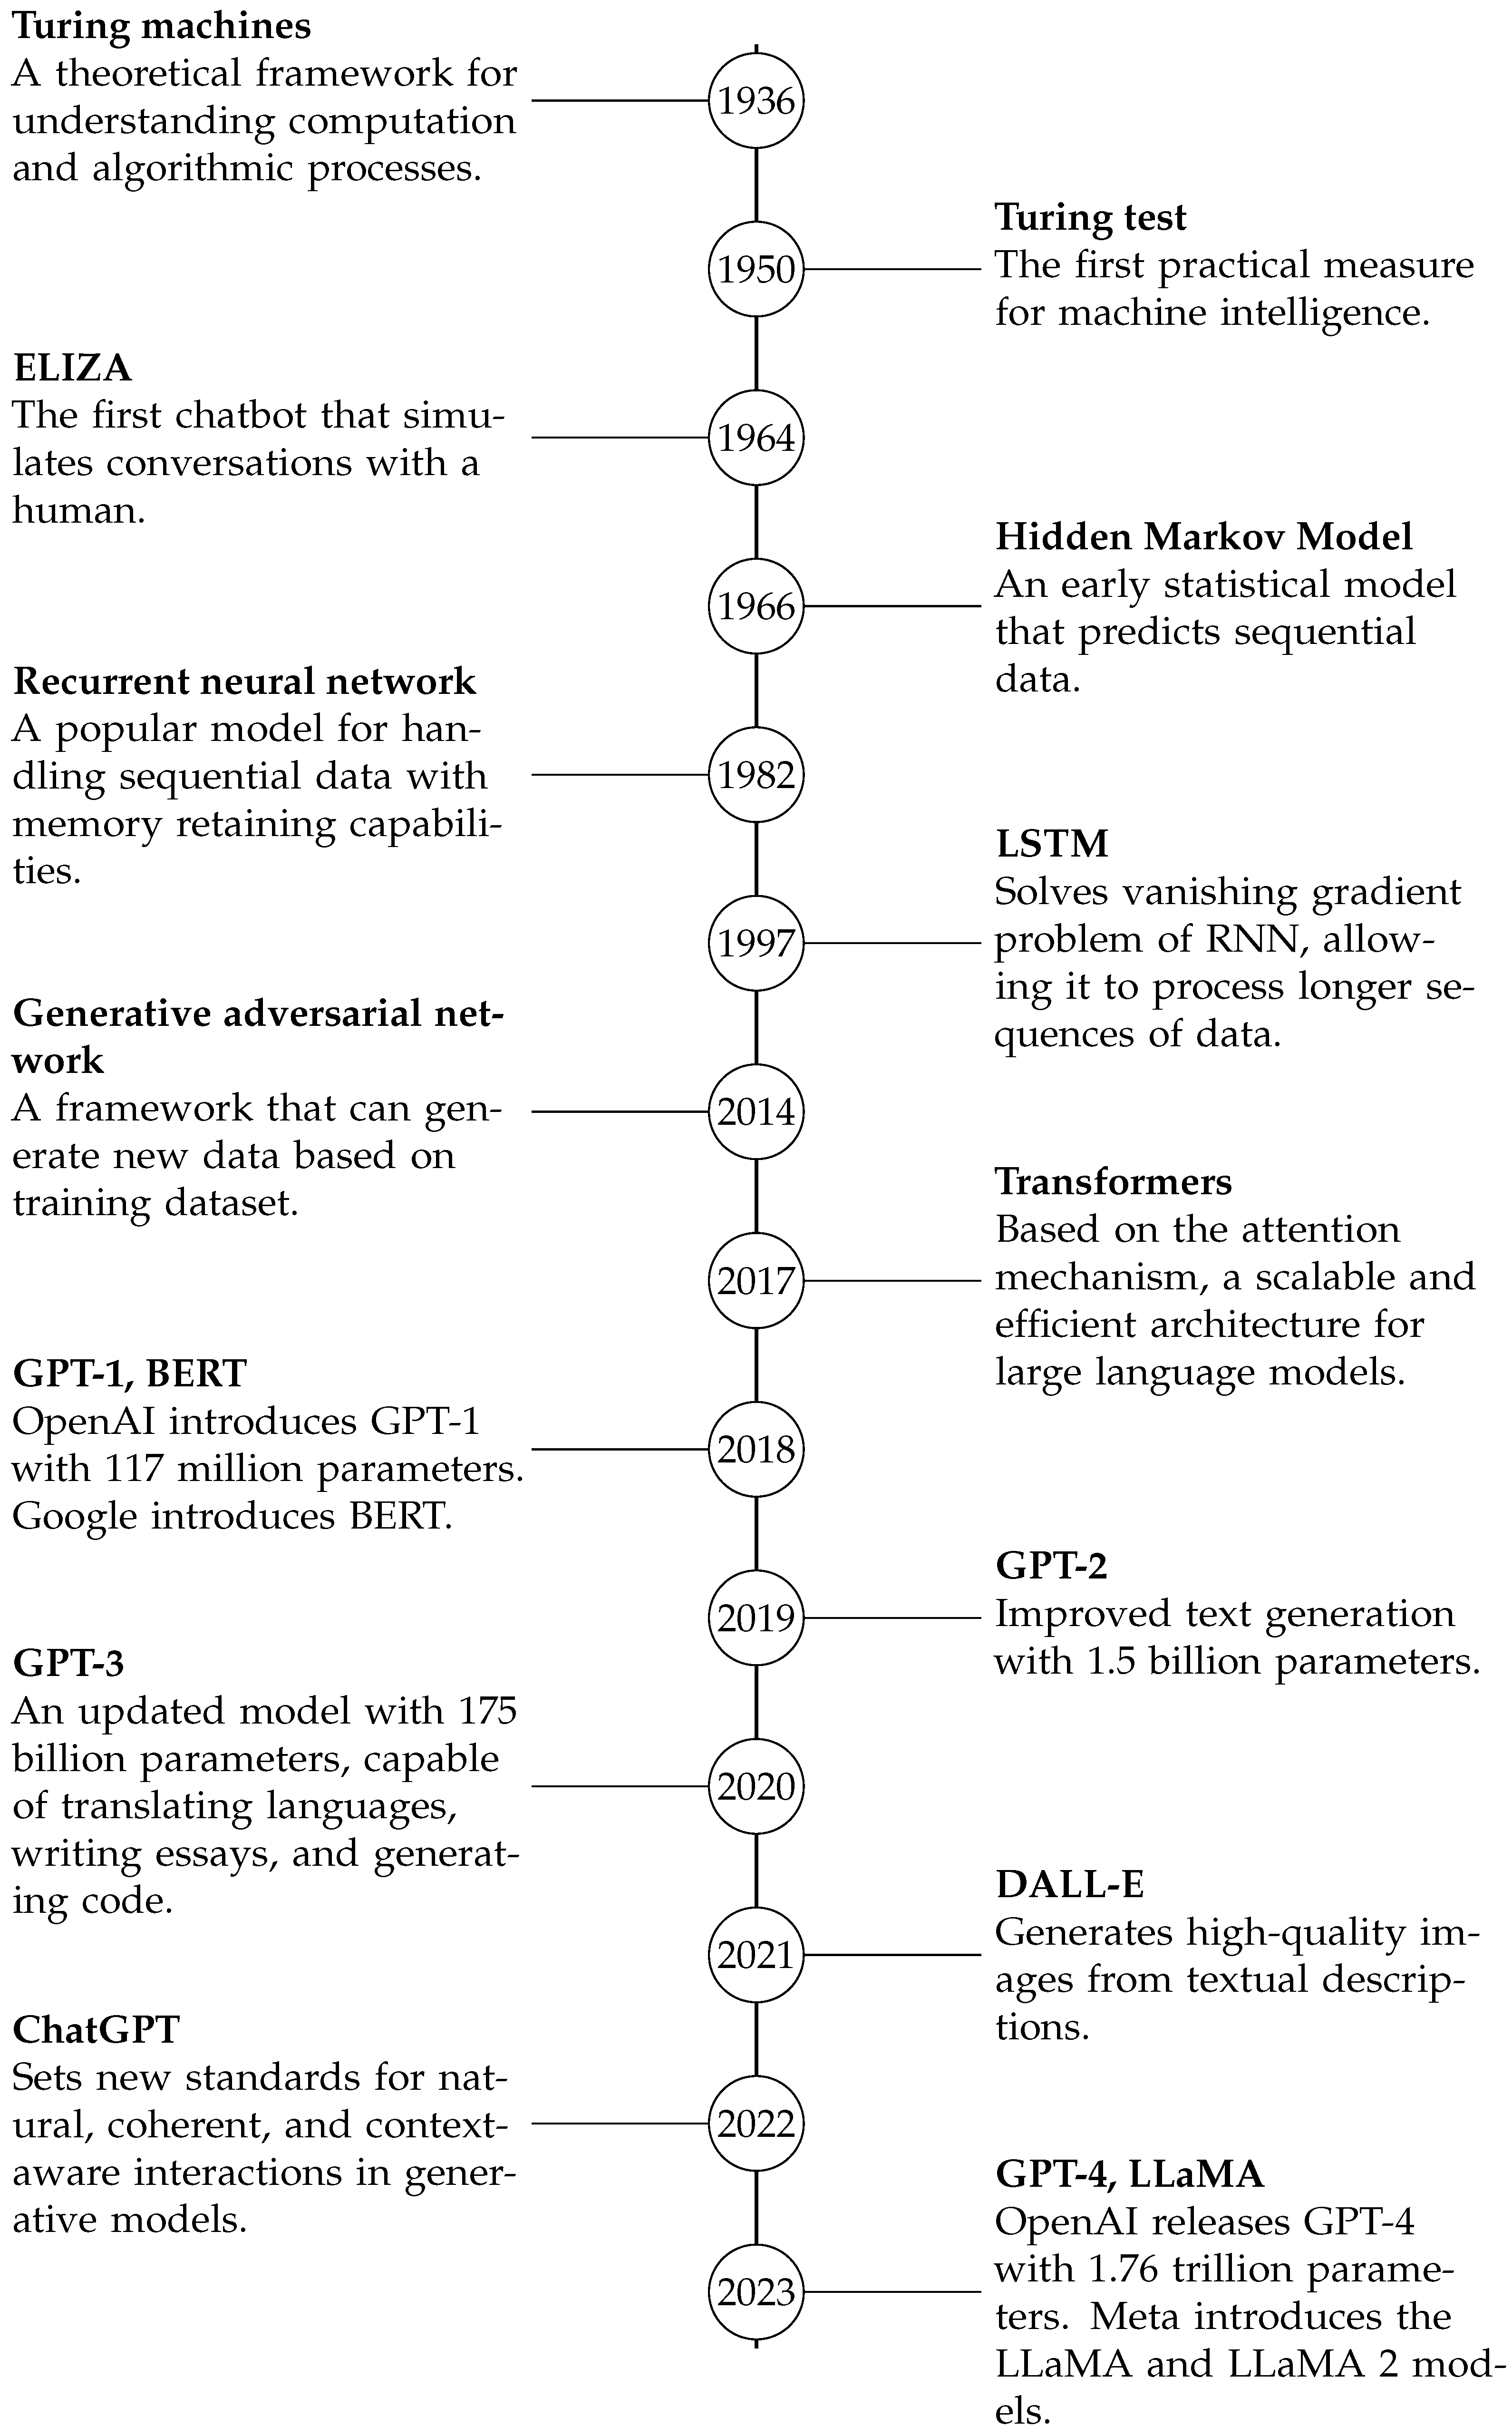
\includegraphics[width=0.3\textwidth]{Immagini/AI_story.png}
	\caption{Illustrazione della linea del tempo dello sviluppo della Generative AI, dalla Macchina di Turing fino a GPT-4 \cite{zhang2023turing}.}
	\label{fig:Generative_AI_story}
\end{figure}

\section{Generative AI sul lavoro}
Sin dalla loro introduzione intorno al 1970, i computer si sono imposti prepotentemente nel mondo del lavoro grazie alla loro capacità di eseguire in modo efficiente istruzioni pre-programmate.\\
La computerizzazione ha notevolmente ridotto i tempi di lavoro specialmente in  operazioni di routine, come l'inserimento dei dati, la contabilità e le mansioni nella catena di montaggio, determinando così una diminuzione dei posti di lavoro e  dei salari in questi settori \cite{acemoglu2011skills}.
Allo stesso tempo, questo fenomeno ha incrementato la domanda di lavoratori con abilità di programmazione, analisi dei dati e  di ricerca, portando ad un aumento della disuguaglianza salariale soprattutto negli Stati Uniti \cite{katz1992changes}.\\
In contrasto, le generative AI non richiedono specifiche istruzioni per eseguire le operazioni, ma possiedono la capacità di imparare dalle esperienze ed applicare le regole incosciamente durante il processo. Questa capacità è definita conoscenza tacita e permette di svolgere operazioni che prevedono di fare affidamento sul giudizio e sull'esperienza del modello \cite{fischer2009michael} \cite{nguyen2022empirical}.
I modelli di diffusione ed i transformers hanno avuto un grande impatto nel mondo del lavoro, trovando diverse applicazioni in vari settori grazie alla loro versatilità.

\section{Modelli di diffusione}
I modelli di diffusione sono una classe di modelli generativi che hanno lo scopo di interpretare distribuzioni di dati molto complesse.
Per ottenere uno di questi modelli si devono affrontare due fasi: la diffusione in avanti e la diffusione all'indietro.
Il primo processo serve per alterare l'architettura di distribuzione dei dati, aumentando gradualmente il livello del rumore all'interno dei dati di input fino ad ottenere un rumore gaussiano puro.
Il processo di diffusione all'indietro effettua l'operazione inversa, fornendo così un modello generativo molto flessibile e capace di generare complesse distribuzioni di dati a partire da un rumore casuale \cite{shokrollahi2023comprehensive}.\\
Per esempio, i Denoinsing, Diffusion Probabilistic Models (DDPMs) appartengono a questa classe di modelli e approssimano i parametri di un processo di diffusione utilizzando l'inferenza variazionale per produrre un'immagine di alta qualità.\cite{ho2020denoising}

\subsection{Applicazioni nell'assistenza sanitaria}
L'assistenza sanitaria è il settore in cui si sono verificati i maggiori progressi grazie all'uso dei modelli di diffusione. Le applicazioni possono includere: la ricostruzione di immagini, le traduzione di immagini e la generazione di un'immagine, tra le principali.
\subsubsection{Ricostruzione di immagini}
La \textbf{ricostruzione di immagini} è un processo di conversione di un'insieme di dati di difficile interpretazione in un'immagine target di facile comprensione.
Infatti, ottenere immagini di alta qualità è fondamentale nella immagini mediche, non solo per la riduzione dei rischi per i pazienti ma anche per l'abbassamento dei costi \cite{levac2023mri}.\\
Le normali tecniche per ricavare immagini dettagliate ed alta risoluzione prevedono alte dosi e prolungato tempo di esposizione alle radiazioni, come per esempio nel caso della Tomografia Computerizzata (CT) o la Risonanza Magnetica (MRI). Di conseguenza, sono state sviluppate strategie per ridurre l'esposizione alle radiazioni come l'uso di dosi ridotte o i processi di imaging con campionamento ridotto.
Tuttavia, queste tecniche possono ridurre il rapporto segnale-rumore (SNR) e il rapporto contrasto-rumore (CNR) influenzando la qualità finale dell'immagine. Questo problema può essere risolto applicando la ricostruzione dell'immagine \cite{shokrollahi2023comprehensive}.\\
Nel 2022 è stato introdotto un approccio chiamato MC-DDPM utilizzando il framework DDPM per raffinare la ricostruzione di immagini mediche sotto-campionate.
MC-DDPM è un approccio che potrebbe essere utilizzato anche per la ricostruzione CT e PET \cite{xie2022measurement}.\\
Nel 2023 per la ricostruzione delle immagini MRI è stata introdotta una tecnica chiamata \textbf{Adaptive Diffusion Priors} (AdaDiff).
Il metodo regola in modo dinamico i suoi priors durante la fase di inferenza per allinearsi meglio con la distribuzione dei dati di test migliorando la qualità dell'immagine \cite{gungor2023adaptive}.
\subsubsection{Traduzione di immagini}
La \textbf{traduzione da immagine ad immagine} è invece una tecnica che permette di trasformare un'immagine di un tipo in un'altra immagine di tipo diverso. Infatti, spesso, per ottenere una corretta diagnosi, dopo un CT è necessario effettuare anche un MRI, rendendo il processo più lungo e costoso.
Con l'utilizzo dei modelli di diffusione si può ridurre il tempo di esposizione grazie al miglioramento della flessibilità e della completezza dell'imaging medico.
Le due architetture fondamentali per la traduzione di immagini sono: pix2pix\cite{isola2017image} e CycleGAN\cite{chu2017cyclegan}.\\
Nel 2023 è stato impiegato un modello di diffusione chiamato SynDiff, che ha dimostrato un'elevata efficacia nella traduzione non supervisionata di immagini mediche. Dopo numerosi test, è stato dimostrato che questo metodo ottiene buoni risultati in termini di precisione, riduzione degli artefatti ed efficienza computazionale rispetto ad altri modelli. Le immagini generate risultano indistinguibili rispetto a quelle originali \cite{ozbey2023unsupervised}.
\subsubsection{Generazione di immagini}
La generazione di immagini è stata una delle prime applicazioni all'interno della sanità, soprattutto per la fabbricazione di immagini mediche artificiali 2D/3D.
Medfusion è un DDPM condizionale latente, utilizzato per la sintesi di immagini mediche. Nel lavoro di \cite{muller2023multimodal} è stata condotta un'analisi approfondita di dataset comprendenti immagini RGB del fondo oculare, scansioni CT del torace e scansioni MRI 3D del cervello di diversi soggetti. Gli autori hanno impiegato diverse metriche di valutazione della qualità delle immagini, tra cui il Peak Signal-to-Noise Ratio (PSNR), il Structural Similarity Index (SSIM) e la Fréchet Inception Distance (FID). I risultati della loro ricerca hanno dimostrato che l'approccio adottato offre una maggiore stabilità e interpretabilità, nonché una qualità superiore delle immagini rispetto ai modelli Generative Adversarial Networks.

\section{Transformers}
\subsection{Definizione di Transformers}
I Generative Transformers (GT) sono un'estensione delle reti neurali e sono designati a pesare il significato delle diverse parti di una sequenza di input, catturando le relazioni intricate tra i dati. Con un corretto addestramento ed il giusto contesto i GT possono generare ogni tipo di dato \cite{zhang2023turing}.
\subsection{Vantaggi dei Transformers rispetto alle CNNs e RNNs nell'Intelligenza Artificiale}
Questi modelli sono stati originariamente progettati per lo sviluppo del Natural Language Processing (NLP), ma successivamente sono stati adattati e applicati anche ad altri ambiti, come ad esempio la Computer Vision \cite{han2022survey}.
I transformers, grazie alla loro architettura avanzata e alla capacità di catturare relazioni a lungo raggio nei dati, presentano diversi vantaggi rispetto alle architetture CNNs ed RNNs. In primis, consentono un'elaborazione parallela dei dati e migliorano significativamente l'efficienza computazionale traducendosi in un risparmio di costi e risorse. Inoltre i GT sono in grado di raggiungere minimi locali o globali con un numero inferiore di passi di addestramento. Questo li rende particolarmente efficaci per compiti complessi come per l'elaborazione dei dati del linguaggio naturale.
A differenza delle CNNs e delle RNNs, i transformers non soffrono di problemi legati alle dipendenze a lungo raggio, un limite significativo delle RNNs, che spesso faticano a mantenere informazioni rilevanti su sequenze di dati estese. Inoltre, i transformers evitano il problema della scomparsa o dell'esplosione del gradiente, che può ostacolare il processo di apprendimento nelle reti neurali tradizionali. Questi vantaggi rendono i transformers una scelta preferibile per molte applicazioni di intelligenza artificiale, dalla traduzione automatica al riconoscimento del linguaggio \cite{vaswani2017attention}.

\subsection{Architettura del modello}
\subsubsection{Encoder-Decoder Structure}
I transformers possiedono una struttura encoder-decoder come rappresentato nella figura \ref{fig:Transformer model}.
L'encoder mappa una rappresentazione simbolica di sequenza \((x_1, \ldots, x_n)\) in una rappresentazione continua di sequenza z=\((z_1, \ldots, z_n)\).
È composto da una pila di 6 livelli identici, ognuno dei quali possiede due sottolivelli seguiti da un livello di normalizzazione.
Il primo sottolivello è il meccanismo di multi-head self-attention, mentre il secondo è una normale rete feed-forward completamente connessa.
Il decoder, dato z, genera una sequenza di simboli \((y_1, \ldots, y_n)\), un elemento per volta, che poi saranno consumati come input addizionale per la prossima generazione. La sua struttura è pressoché simile a quella dell'encoder, con ogni livello che possiede un sottolivello aggiuntivo che esegue il multi-head attention sull'output della pila dell'encoder.
Il meccanismo di self-attention viene modificato con una maschera speciale per impedire che le posizioni future possano influenzare le posizioni attuali, quindi la previsione per \(y_i\) non dipende dalle posizioni future \( y_{i+1}, y_{i+2}, \ldots \), e il contesto prevede solo i simboli già generati fino a quel punto \cite{vaswani2017attention}.

\begin{figure}[ht]
	\centering
	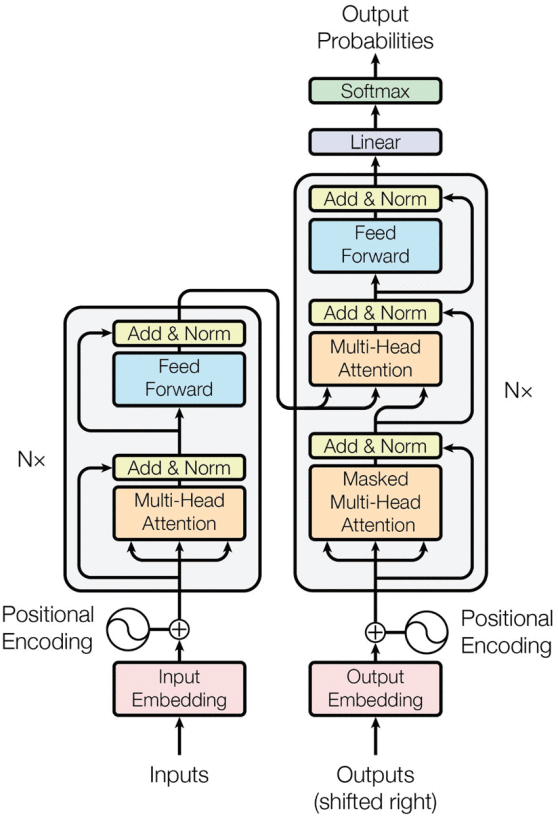
\includegraphics[width=0.3\textwidth]{Immagini/transformers.png}
	\caption{Transformer - architettura del modello \cite{vaswani2017attention}.}
	\label{fig:Transformer model}
\end{figure}

\subsubsection {Il Meccanismo Attention}
É un meccanismo che consente di capire il contesto della parola estrapolandolo dalla parte più significativa dell'input.
La funzione attention può essere rappresentata come una mappatura tra una query ed un'insieme di coppie chiave valore e l'output.
L'output è la somma pesata di tutti i valori, dove il peso di ogni valore è calcolato dalla funzione di compatibilità della query con la chiave corrispondente.
La funzione di attention permette di calcolare simultaneamente un'insieme di query, nella formula \ref{equ:attention} viene determinato l'output della funzione.

\begin{equation*} Attention(Q, K, V) = softmax\left ({{\frac {QK^{T}}{\surd d_{k}}}}\right)V \tag {6} \label{equ:attention} \end{equation*}

Dove Q rappresenta l'insieme di query, K l'insieme delle chiavi nella matrice e V l'insieme dei valori nella matrice.
Per evitare che la funzione Softmax sia indirizzata verso zone di gradiente estremamente piccole a causa di un fattore di scala molto grande, nella formula \ref{equ:attention} Il fattore di scala \(d_k\) viene sostituito con \(\frac{1}{d_k}\) \cite{vaswani2017attention}.

\begin{figure}[ht]
	\centering
	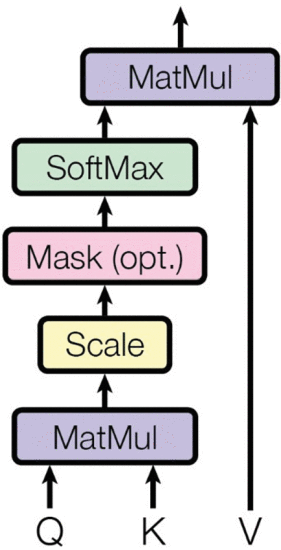
\includegraphics[width=0.3\textwidth]{Immagini/self_attention_dot.png}
	\caption{Scaled Dot-Product Attention \cite{vaswani2017attention}}
	\label{fig:Scaled Dot-Product Attention}
\end{figure}

Multi-Head Attention permette al modello di imparare diversi significati della sequenza di input, in questo modo il meccanismo di self-attention può essere eseguito molteplice volte in parallelo.
Ogni esecuzione parallela è chiamata testa. Ogni testa esplora l'input attraverso una diversa prospettiva o "sotto-spazio di rappresentazione", permettendo al modello di apprendere diverse relazioni tra gli elementi.
La formula \ref{equ:multihead_attention} mostra come gli attention output indipendenti sono concatenati e linearmente trasformati nella dimensione aspettata \cite{vaswani2017attention}.

\begin{equation*} MultiHead\left ({{ Q, K, V }}\right)=concat\left ({{ {head}_{1},\ldots {head}_{h} }}\right)W^{o} \tag {7} \label{equ:multihead_attention} \end{equation*}

dove \(\text{head}_i = \text{Attention}(QW_i^Q, KW_i^K, VW_i^V)\)

\begin{figure}[ht]
	\centering
	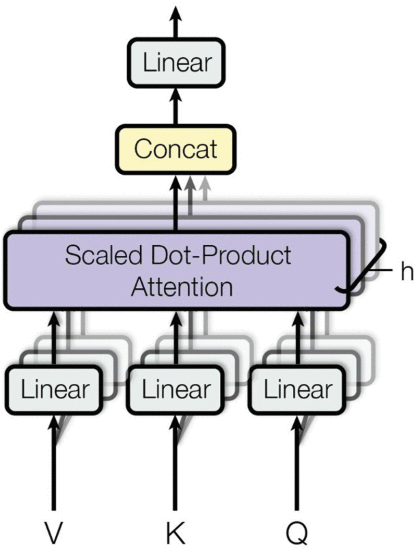
\includegraphics[width=0.3\textwidth]{Immagini/Multi-Head.png}
	\caption{ Scaled Dot-Product Multi-Head Attention \cite{vaswani2017attention}.}
	\label{fig:Multi-Head}
\end{figure}
\chapter{Large Language Models (LLMs)}

\section{Introduzione e caratteristiche degli LLMs}
Un modello di linguaggio di grandi dimensioni (Large Language Model, LLM) è un tipo di modello di intelligenza artificiale caratterizzato da un numero estremamente elevato di parametri e addestrato su un vasto corpus di dati testuali. Questi modelli sono progettati per eseguire operazioni linguistiche con un elevato grado di accuratezza.\newline
L'architettura Transformer ha giocato un ruolo cruciale nel successo di questi modelli. Il meccanismo di self-attention, che costituisce la base di questa architettura, consente di valutare l'importanza relativa delle diverse parti dell'input e di comprendere le relazioni tra le parole in modo più efficace rispetto alle architetture precedenti.\newline
Un ulteriore elemento chiave del successo degli LLM è rappresentato dal processo di pre-addestramento. Questo processo utilizza un vasto insieme di dati, che può includere articoli, libri e altre forme di testo, per formare il modello a eseguire operazioni linguistiche con maggiore competenza. Il pre-addestramento su dati di larga scala permette al modello di acquisire una comprensione approfondita delle strutture linguistiche e delle conoscenze generali, che vengono poi affinati per compiti specifici attraverso un processo di addestramento mirato \cite{kasneci2023chatgpt}.

\section{Esempi di LLMs attuali}

\subsection{Panoramica dei modelli LLMs}
La tabella \ref{LLMs} presenta diversi modelli di linguaggio e le loro rispettive caratteristiche. La colonna "tunability" indica i modelli che possono essere sottoposti a fine-tuning per compiti specifici, al fine di migliorarne l'efficacia per tali compiti \cite{yao2024survey}. Tra i modelli, si possono osservare le diverse versioni di GPT, che nel tempo hanno ottenuto un successo particolare.

\begin{table}[ht]
    \centering
    \resizebox{0.99\linewidth}{!}{
        \begin{tabular}{||c||c|c|c|c|c||}
            \hline
            Modello & Data & Azienda & Open-Source & Parametri & Tunability \\
            \hline
            GPT-4 \cite{achiam2023gpt} & 2023.03 & OpenAI & NO & 1.7 T & NO \\
            \hline
            GPT-3.5-turbo & 2021.09 & OpenAI & NO & 175 B & NO \\
            \hline
            Cohere-medium \cite{liang2022holistic} & 2022.07 & Cohere & NO & 6 B & YES \\
            \hline
            Cohere-large \cite{liang2022holistic} & 2022.07 & Cohere & NO & 13 B & YES \\
            \hline
            Cohere-xlarge \cite{liang2022holistic} & 2022.07 & Cohere & NO & 52 B & YES \\
            \hline
            BERT \cite{devlin2018bert} & 2018.08 & Google & YES & 340 M & YES \\
            \hline
            T5 \cite{raffel2020exploring} & 2019 & Google & YES & 11 B & YES \\
            \hline
            PaLM \cite{narang2022pathways} & 2022.04 & Google & YES & 540 B & YES \\
            \hline
            LLaMA \cite{meta2023introducing} & 2023.02 & Meta AI & YES & 65 B & YES \\
            \hline
            CTRL \cite{keskar2019ctrl} & 2019 & Salesforce & YES & 1.6 B & YES \\
            \hline
            Dolly 2.0 & 2023.04 & Databricks & YES & 12 B & YES \\
            \hline
        \end{tabular}
    }
    \vspace*{2mm}
    \caption{Confronto tra i diversi modelli di linguaggio \cite{yao2024survey}}
    \label{LLMs}
\end{table}

\subsection{Generative Pre-trained Transformer (GPT)}
GPT è un modello di linguaggio autoregressivo che genera sequenze di parole, codice ed altre forme di dato, partendo da una sorgente di input, chiamata prompt.
Il modello è stato addestrato utilizzando il supercomputer Microsoft Azure AI, con costi stimati intorno ai 12 milioni di dollari. La prima iterazione risale al 2018 e ha impiegato 110 milioni di parametri. L'anno successivo, GPT-2 ha utilizzato 1,5 miliardi di parametri, mentre GPT-3 ne utilizza infine 175 miliardi \cite{floridi2020gpt}.
Il modello più recente, GPT-4, è stato addestrato con 1 trilione di parametri, e OpenAI sta già lavorando allo sviluppo di GPT-5.

\subsubsection{GPT-4 Performance}
La \textbf{perdita finale} di un modello può essere approssimata utilizzando leggi di scala, in questo modo riusciamo a prevedere la relazione tra le risorse computazionali impiegate e la performance del modello \cite{achiam2023gpt}.
Nella figura \ref{fig:loss-prediction}, è stata analizzata la perdita finale di GPT-4 utilizzando un dataset molto ampio di codici non incluso nell'insieme di addestramento, impiegando la legge di scala \ref{equ:scaling} \cite{henighan2020scaling}.

\begin{equation}
    L(C) = aC^b + c
    \label{equ:scaling}
\end{equation}

Dove \textbf{a} è una costante che determina l'ampiezza dell'effetto della variabile \textbf{C}, che rappresenta una misura della risorsa computazionale o della dimensione del modello, come il numero di parametri o la dimensione del dataset. \textbf{b} è l'esponente che indica come la perdita dipende dalla variabile C, ed infine \textbf{c} è una costante aggiuntiva che rappresenta un termine di perdita asintotica o residua.
La previsione è basata utilizzando modelli addestrati nello stesso modo, ma utilizzando 10.000 volte meno calcolo di GPT-4 come mostrato nella figura \ref{fig:loss-prediction} \cite{achiam2023gpt}.
\begin{figure}[ht]
	\centering
	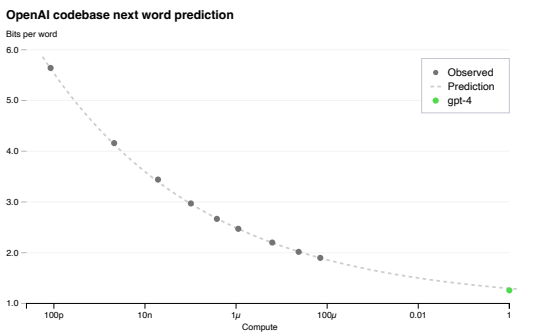
\includegraphics[width=0.3\textwidth]{Immagini/GPT-4_word_prediction.png}
	\caption{ Performance di GPT-4 e modelli più piccoli. La metrica è la perdita finale su un dataset interno, la linea tratteggiata corrisponde alle legge adattata ai modelli più piccoli, predicendo con precisione la perdita finale di GPT-4. L'asse x rappresenta il calcolo di addestramento normalizzato in modo che GPT-4 sia uguale a 1 \cite{achiam2023gpt}.}
	\label{fig:loss-prediction}
\end{figure}

È stato utilizzato il dataset HumanEval \cite{chen2021evaluating} per valutare metriche di capacità, come ad esempio il tasso di successo. Il test prevedeva di misurare la sintesi di funzioni Python di varia complessità. La previsione del tasso di successo su un sottoinsieme del dataset HumanEval è stata effettuata estraendo dati da modelli addestrati con al massimo 1.000 volte meno calcolo. Poiché la performance potrebbe deteriorarsi con la scala per un singolo problema nel dataset, la relazione approssimativa di legge di potenza \ref{equ:power_law} cerca di affrontare questo problema \cite{achiam2023gpt}.

\begin{equation}
- \mathbb{E}_P \left[ \log(\text{pass\_rate}(C)) \right] = \alpha C^{-k}
\label{equ:power_law}
\end{equation}

Dove k e \(\alpha\) sono costanti positive e P rappresenta il sottoinsieme dei problemi presi da HumanEval dataset.
L'obiettivo era prevedere la performance di GPT-4 sul dataset prima che l'addestramento fosse completato, basandosi sui risultati dei modelli più piccoli. I problemi sono stati suddivisi dai modelli più piccoli in sei categorie di difficoltà. La figura \ref{fig:pass-rate} mostra i risultati della categoria numero 3, dove era possibile stimare con precisione il logaritmo del tasso di successo utilizzando i modelli più piccoli; anche le altre categorie hanno comunque ottenuto prestazioni molto buone. GPT-4 ha sottoperformato nelle categorie più facili, mentre ha ottenuto risultati migliori nelle categorie che contenevano classi di problemi più difficili \cite{achiam2023gpt}.

\begin{figure}[ht]
	\centering
	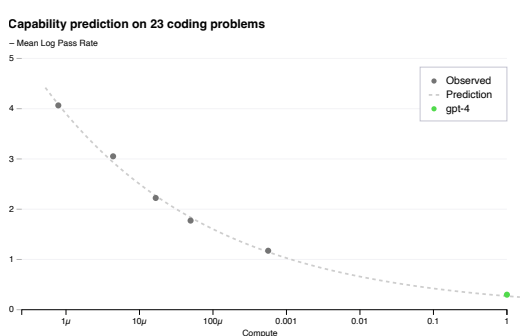
\includegraphics[width=0.3\textwidth]{Immagini/GPT-4_coding_problems.png}
	\caption{ Performance di GPT-4 e modelli più piccoli. La metrica è la media del logaritmo del tasso di successo su un sottoinsieme di HumanEval. L'asse x rappresenta il calcolo di addestramento normalizzato in modo che GPT-4 sia pari a 1 \cite{achiam2023gpt}.}
	\label{fig:pass-rate}
\end{figure}

GPT-4 è stato testato su esami umani senza addestramento specifico per questi.
Le domande includevano vari formati (scelta multipla e risposta libera) e sono stati utilizzati prompt specifici per ciascun tipo.
I punteggi sono stati calcolati combinando i risultati delle diverse tipologie di domande e i percentili sono stati stimati e riportati nella figura \ref{fig:exam-results} \cite{achiam2023gpt}.

\begin{figure}[H]
	\centering
	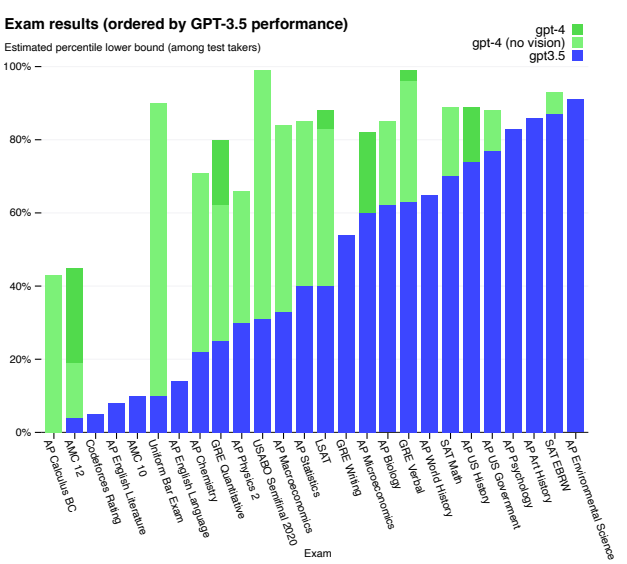
\includegraphics[width=0.3\textwidth]{Immagini/exam_results.png}
	\caption{ performance di GPT-4 su esami accademici e professionali, simulando le condizioni e il sistema di valutazione degli esami reali \cite{achiam2023gpt}.}
	\label{fig:exam-results}
\end{figure}

Nella figura \ref{fig:GPT4-benchmarks} si possono osservare le prestazioni di GPT-4 sui benchmark tradizionalmente utilizzati per valutare i modelli linguistici di grandi dimensioni, ottenendo infine ottimi risultati in confronto ad essi \cite{achiam2023gpt}.\\

\begin{figure}[ht]
	\centering
	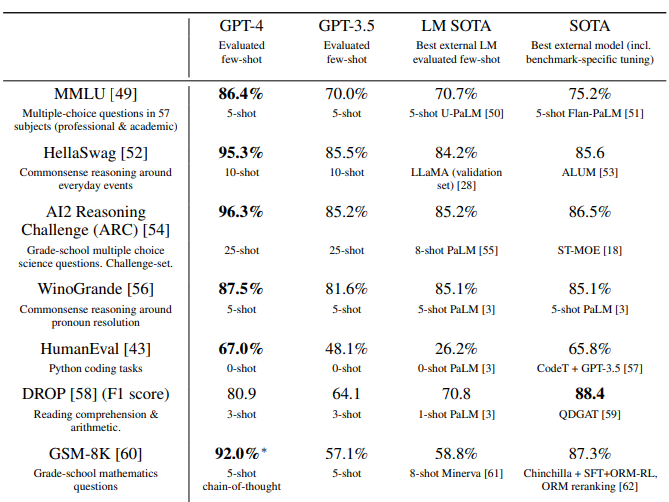
\includegraphics[width=0.3\textwidth]{Immagini/GPT-4_benchmarks.png}
	\caption{ prestazioni di GPT-4 su benchmarks accademici \cite{achiam2023gpt}.}
	\label{fig:GPT4-benchmarks}
\end{figure}

La maggior parte dei ML benchmarks sono scritti in inglese, quindi gli MMLU benchmarks\footnote{un'insieme di problemi a scelta multipla di 57 discipline diverse} sono stati tradotti in altre lingue e testati.
Nella figura \ref{fig:GPT4-languages-benchmarks} possiamo osservare i risultati dei test tra GPT-4 e gli altri modelli di linguaggio. GPT-4 ha superato di gran lunga le prestazioni del modello precedente e di tutti gli altri modelli, sia in inglese che in tutte le altre lingue \cite{achiam2023gpt}.

\begin{figure}[ht]
	\centering
	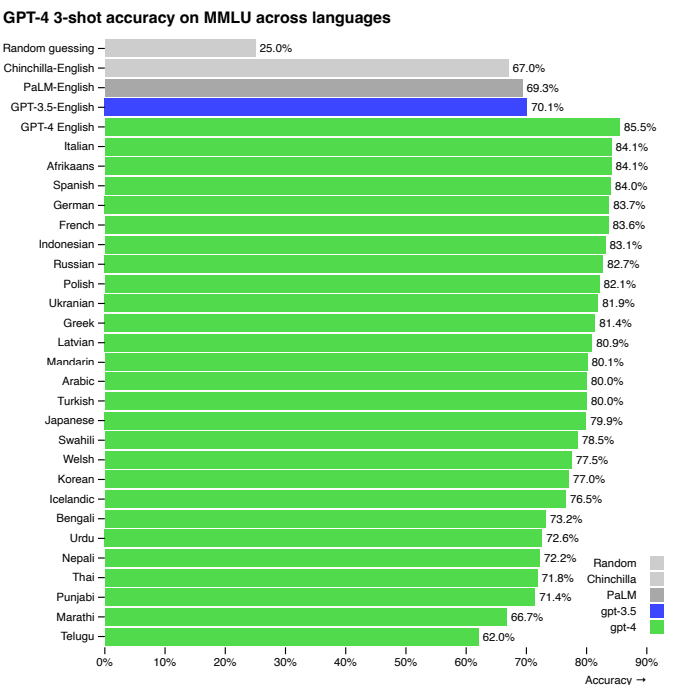
\includegraphics[width=0.3\textwidth]{Immagini/GPT-4_languages_benchmarks.png}
	\caption{ prestazioni di GPT-4 sui MMLU benchmarks tradotti in altre lingue in confronto ad altri modelli \cite{achiam2023gpt}.}
	\label{fig:GPT4-languages-benchmarks}
\end{figure}

In conclusione, nonostante i risultati eccezionali ottenuti da GPT-4, il modello non è ancora completamente affidabile, poiché può generare fatti inesatti ("allucinazioni") e commettere errori di ragionamento. È quindi necessario prestare sempre attenzione e fare un uso attento e consapevole dello strumento \cite{achiam2023gpt}.

\subsection{Google Gemini}
Gemini è il modello multimodale nativo\footnote{Modello di intelligenza artificiale progettato per comprendere e generare dati attraverso diversi tipi di input e output, come testo, immagini, audio e video, in modo nativo. Questo significa che il modello è stato concepito e addestrato fin dall'inizio per lavorare con più modalità di dati, piuttosto che essere un modello originariamente unimodale (ad esempio solo testuale) che è stato successivamente adattato per gestire altre modalità.} sviluppato da Google. La capacità di processare insiemi di dati complessi, come grafici e immagini, consente a questo modello di trovare applicazione in ambiti come la medicina e l'oftalmologia. In medicina, oltre alla sua abilità nell'analisi delle immagini, Gemini è in grado di comprendere e interpretare la letteratura medica, lo storico dei pazienti e i dati di ricerca. In oftalmologia, Gemini può diagnosticare condizioni oculari, analizzare i sintomi riportati dai pazienti e suggerire piani di trattamento basati su ricerche recenti e linee guida cliniche \cite{masalkhi2024google}.
Al contrario, modelli di linguaggio come ChatGPT possono avere difficoltà nella comprensione del contesto delle informazioni o nel fornire dati aggiornati, rendendo complesso l'utilizzo di queste tecnologie in ambiti specialistici \cite{waisberg2023bridging} \cite{kocon2023chatgpt} \cite{jeyaraman2023chatgpt} \cite{waisberg2023chatgpt}.

\section{Impatti e Applicazioni degli LLMs}
\subsection{Applicazioni nel business e nella finanza}
Nei recenti studi di \cite{chen2023fiction} è stato condotto un esperimento per dimostrare l'abilità di ChatGPT nel condurre un'analisi del sentiment nel mercato finanziario. Nel 2013, in California, è entrato in vigore il programma cap-and-trade per ridurre le emissioni di gas serra. Sono state esaminate 321 aziende con sede in California, Nevada, Oregon e Arizona, utilizzando i rapporti annuali delle aziende successivi all'approvazione della politica nel 2011. È stato fornito a ChatGPT il seguente prompt template per attribuire un punteggio al sentiment negativo: \textit{'On a probability scale of 0 to 1, what is the negative sentiment score of the discussion for capand-trade policy in the provided text:’ + ‘searched text’ + ‘Please only output the sentiment score without any narrative nor analysis. So the sentiment score of this text is: '}
La figura \ref{fig:sentiment-analysis} mostra come le aziende con punteggi di sentiment negativo più alti abbiano registrato ritorni giornalieri più bassi (0.06) rispetto a quelle con punteggi di sentiment negativo più bassi (0.14). Inoltre, le aziende che non hanno menzionato le parole chiave hanno avuto i valori di ritorno più bassi e fluttuazioni maggiori nei ritorni (-0.12 e deviazione standard di 2.04).

\begin{figure}[ht]
	\centering
	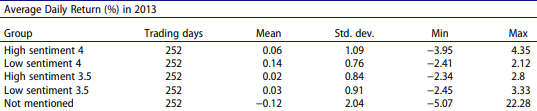
\includegraphics[width=0.3\textwidth]{Immagini/sentiment_analysis.png}
	\caption{ Valori di ritorno per ogni categoria del sentiment negativo generato da GPT-3.5 E GPT-4 \cite{chen2023fiction}.}
	\label{fig:sentiment-analysis}
\end{figure}
Il case study ha dimostrato che dopo aver introdotto una politica aziendale, il sentiment negativo delle aziende, rilevato da ChatGPT, ha predetto una migliore capacità di gestione del rischio e una performance azionaria meno volatile.
Il sentiment negativo generato da ChatGPT può indicare efficacemente i fattori di rischio.
Nel settore finanziario è fondamentale considerare le limitazioni dei modelli utilizzati. I dati generati da un modello potrebbero condurre ad addestramenti errati dei modelli stessi, decisioni fuorvianti e significative perdite economiche. Inoltre, è importante tenere presente che le predizioni si basano su dati storici e non sono in grado di prevedere eventi inaspettati. Un ulteriore limite risiede nella variabilità delle risposte: domande con lo stesso significato, ma formulate in modo diverso, possono ottenere risposte differenti.

\subsection{Applicazioni e benefici nella medicina}
Gli studi condotti da \cite{zheng2024large} hanno messo in luce i molteplici vantaggi derivanti dall'impiego dei modelli linguistici di grandi dimensioni nel campo medico. Tra questi, spiccano la capacità di migliorare la diagnosi e la previsione delle patologie, l'integrazione della conoscenza e l'accesso in tempo reale alle informazioni, lo sviluppo di trattamenti personalizzati e di farmaci, la gestione ottimizzata dei pazienti e dei processi sanitari, nonché il potenziamento dell'educazione clinica e la diffusione della conoscenza medica.

\subsubsection{Capacità di diagnosi e previsione migliorate}
Gli LLMs facilitano la diagnosi precoce e la previsione delle malattie, consentendo interventi tempestivi e personalizzati. Essi sono anche in grado di prevedere l'efficacia dei trattamenti basati su dati clinici e genomici.

\subsubsection{Integrazione della conoscenza e accesso in tempo reale}
Gli LLMs aggiornano costantemente il corpus delle conoscenze mediche globali, supportando decisioni cliniche basate sulle più recenti evidenze e migliorando la precisione sia diagnostica che terapeutica.

\subsubsection{Trattamenti personalizzati e sviluppo di farmaci}
Gli LLMs sono in grado di elaborare piani terapeutici su misura per i singoli pazienti e accelerano il processo di sviluppo di nuovi farmaci, prevedendone l'efficacia e i possibili effetti collaterali.

\subsubsection{Gestione dei pazienti e ottimizzazione dei processi sanitari}
Gli LLMs contribuiscono alla personalizzazione della gestione della salute dei pazienti e al miglioramento dell'efficienza dei processi sanitari, attraverso l'identificazione e l'ottimizzazione dei punti critici nei flussi di lavoro.

\subsubsection{Educazione clinica e diffusione della conoscenza medica}
Gli LLMs rivestono un ruolo fondamentale nell'ambito dell'educazione medica, simulando scenari clinici realistici e fornendo applicazioni sanitarie che offrono consigli personalizzati per la prevenzione e la gestione delle malattie, aiutando così i pazienti a prendere decisioni informate riguardo alla propria salute.

\subsubsection{Applicazioni e Supporto degli LLM in Diverse Specialità Mediche}
Gli LLM medici hanno ottenuto notevole successo nei seguenti settori: odontoiatria \cite{huang2023chatgpt}, radiologia \cite{d2024large}, medicina nucleare \cite{wang2023huatuo}, clinica \cite{singhal2023large} e progettazione dei farmaci \cite{chakraborty2023artificial}. Inoltre, hanno fornito supporto in ambiti quali la medicina interna \cite{omiye2024large}, la chirurgia \cite{puladi2023impact}, l'ostetricia e ginecologia \cite{grunebaum2023exciting}, le malattie infettive \cite{schwartz2024black}, la medicina genetica \cite{feldman2019development} e le malattie croniche \cite{biswas2023role}. Gli LLM medici sono addestrati su ampi corpus di dati biomedici, BioGPT \cite{luo2022biogpt} e BioBERT \cite{lee2020biobert} sono esempi rappresentativi di tali modelli.
BioBERT, rispetto ad altri modelli, ha dimostrato di migliorare del 0,62\% il punteggio F1 nella riconoscimento delle entità all'interno dei testi biomedici, come geni, proteine e malattie. Inoltre, ha aumentato del 2,80\% il punteggio F1 nell'estrazione delle relazioni tra entità nei testi biomedici e ha ottenuto un miglioramento del 12,24\% nel Mean Reciprocal Rank per la risposta a query relative ad argomenti biomedici \cite{zheng2024large}.
Le applicazioni degli LLMs sono mostrati nella figura \ref{fig:llms-medicine} e nella tabella \ref{tab:medical-LLMs} sono elencati alcuni dei LLM medici ed i loro casi d'uso.

\begin{figure}[ht]
	\centering
	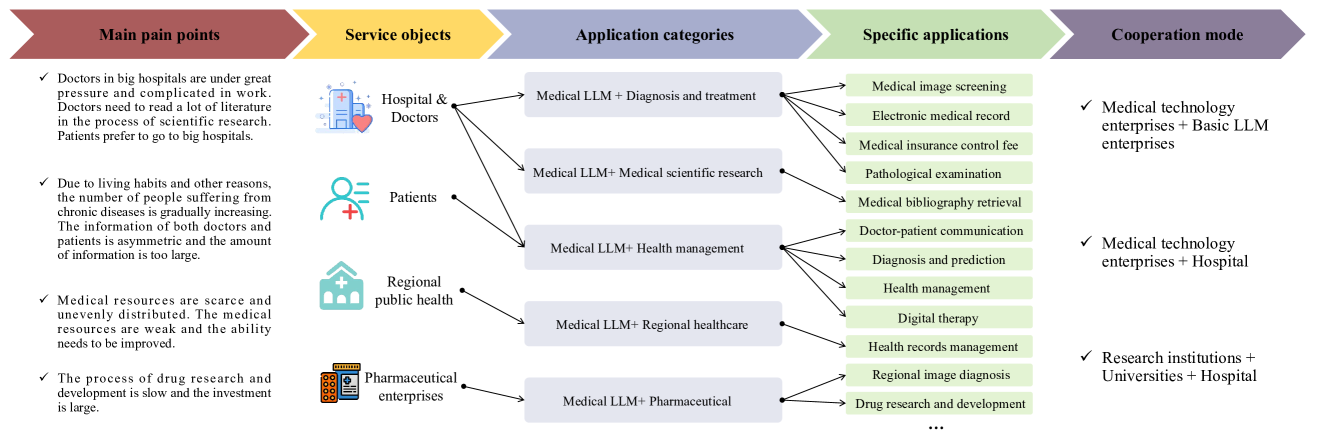
\includegraphics[width=0.3\textwidth]{Immagini/medicine_applications.png}
	\caption{ I punti critici delle cure mediche e le applicazioni dei LLM medici \cite{zheng2024large}.}
	\label{fig:llms-medicine}
\end{figure}
\begin{table}[ht]
	\centering
	\resizebox{0.99\linewidth}{!}{
	\begin{tabular}{||c||c|c|c|c||}
        \hline        Dominio&\phantom{00}LLM\phantom{00}&\phantom{00}Anno\phantom{00}&\phantom{00}Articolo\phantom{00}&\phantom{00}Sorgente\phantom{00} \\
        \hline
		\multirow{7}{*}{Terapia integrativa e diagnosi}
                &MedGPT&2021&\cite{kraljevic2021medgpt}&\url{https://medgpt.co/home} \\
                &LLM-Mini-CEX&2023&\cite{shi2023llm}&  \\
                &WiNGPT&2023&/&\url{https://github.com/winninghealth/WiNGPT2}\\
                &SkinGPT-4&2023&\cite{zhou2023skingpt}& \\
                &DoctorGLM&2023&\cite{xiong2023doctorglm}&\url{https://github.com/xionghonglin/DoctorGLM} \\
                &BenTsao (Huatuo)&2023&\cite{wang2023huatuo}&\url{https://github.com/SCIR-HI/Huatuo-Llama-Med-Chinese} \\
                &ClinicalGPT&2023&\cite{wang2023clinicalgpt}& \\             
        \hline
        \hline
            \multirow{4}{*}{Progettazione faramci}
            &PanGu Drug Model&2023&\cite{lin2022pangu}& \\
            &HelixFold-Single&2023&\cite{fang2023method}&\url{https://github.com/PaddlePaddle/PaddleHelix/tree/dev/apps/protein_folding/helixfold-single}\\
            &TransAntivirus&2023&\cite{mao2023transformer}& \\
            &OpenBioMed&2023&\cite{luo2023towards}&\url{https://github.com/PharMolix/OpenBioMed} \\           
        \hline
        \hline
            \multirow{4}{*}{segmentazione delle immagini mediche}
            &DSI-Net&2021&\cite{zhu2021dsi}&\url{https://github.com/CityU-AIM-Group/DSI-Net}\\
            &MedLSAM&2023&\cite{lei2023medlsam}&\url{https://github.com/openmedlab}\\
            &Lvit&2023&\cite{li2023lvit}&\url{https://github.com/HUANGLIZI/LViT}\\
            &MedCLIP-SAM&2024&\cite{koleilat2024medclip}& \\
        \hline

        \hline
            \multirow{6}{*}{Comunicazione dottore-paziente}
            &BioMedLM/PubMed GPT&2022&/&\url{https://www.databricks.com/blog/category/generative-ai/mosaic-research}\\
            &ChatDoctor&2023&\cite{li2023chatdoctor}&\url{https://github.com/Kent0n-Li/ChatDoctor} \\
            &Disc-medllm&2023&\cite{bao2023disc}&\url{https://github.com/FudanDISC/DISC-MedLLM}\\
            &BianQue&2023&\cite{chen2023bianque}&\url{https://github.com/scutcyr/BianQue}\\
            &MeChat&2023&\cite{qiu2023smile}&\url{https://github.com/qiuhuachuan/smile}\\
            &PMC-LLaMA&2023&\cite{wu2024pmc}&\url{https://github.com/chaoyi-wu/PMC-LLaMA}\\
        \hline
        \hline
            \multirow{3}{*}{Multimodale}
            &OpenMEDLab&2023&/&\url{https://github.com/openmedlab}\\
            &Med-MLLM&2023&\cite{liu2023medical}& \\
            &PeFoMed&2024&\cite{he2024pefomed}&\url{https://github.com/jinlHe/PeFoMed}\\
        \hline

        \hline
            \multirow{4}{*}{Gestione della salute}
            &CIDRS&2021&\cite{wang2021cloud}& \\
            &GatorTron&2022&\cite{yang2022large}&\url{https://catalog.ngc.nvidia.com/orgs/nvidia/teams/clara/models/gatortron_og}\\
            &CareGPT&2023&/&\url{https://github.com/WangRongsheng/CareGPT}\\
            &Bianshi&2023&/&\url{https://www.a-eye.cn/technology.html##Model}\\
        \hline
	\end{tabular}
	}
	\vspace*{2mm}
	\caption{Informazioni sui diversi LLMs medici e il loro campo di applicazione \cite{zheng2024large}.}
	\label{tab:medical-LLMs}
\end{table}

\subsection{Impatti nella Cybersecurity}
I recenti studi condotti da \cite{10198233} mostrano come gli LLMs possono essere un'utile strumento per la cybersecurity ma anche un problema per la privacy e la sicurezza.
La figura \ref{fig:cybersecurity-impact} mostra l'impatto degli LLMs\footnote{nell'articolo si prende come riferimento ChatGPT} all'interno della cybersecurity.

\begin{figure}[ht]
	\centering
	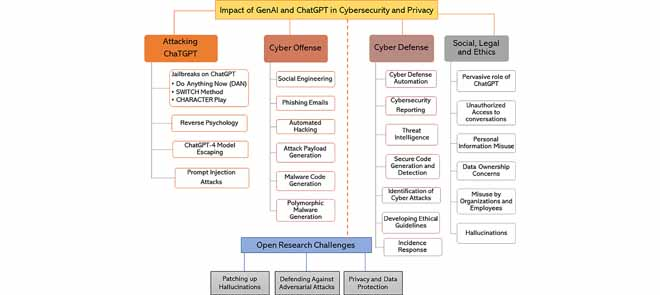
\includegraphics[width=0.3\textwidth]{Immagini/Cybersceurity_impact.jpg}
	\caption{ Riepilogo dell'impatto degli LLMs nella Cybersecurity e strategie future \cite{10198233}.}
	\label{fig:cybersecurity-impact}
\end{figure}
\subsubsection{LLMs per la Cyber Defense}
ChatGPT può essere utilizzato per analizzare incidenti di sicurezza informatica alleggerendo il lavoro della Security Operations Center (SOC), come per esempio l'analisi di uno script Powershell.

\begin{figure}[ht]
	\centering
	\begin{subfigure}{0.3\textwidth}
		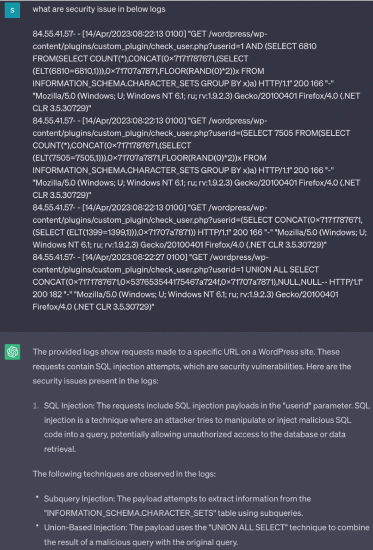
\includegraphics[width=1.0\textwidth]{Immagini/logs_detecting.png}
		\caption{ChatGPT individua problemi di sicurezza nei log di accesso \cite{calbimonte2023powershell}.}
            \label{fig:logs-detecting}
	\end{subfigure}%
	\begin{subfigure}{0.3\textwidth}
		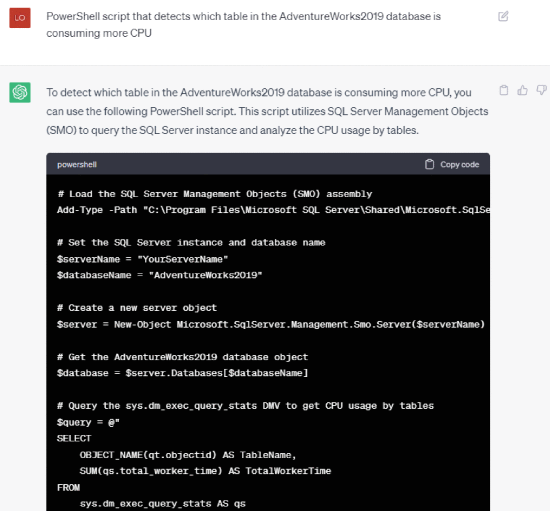
\includegraphics[width=1.0\textwidth]{Immagini/cpu_consuming_detecting.png}
		\caption{PowerShell script che individua quale tabella in AdventureWorks2019 database consuma più cpu \cite{calbimonte2023powershell}.}
            \label{fig:cpu-consuming}
	\end{subfigure}
	\caption{}
\end{figure}

Nella figura \ref{fig:logs-detecting} vengono forniti i log dei server come input a ChatGPT, il quale è in grado di identificare possibili minacce, come ad esempio le SQL injections, e di definirne la categoria \cite{calbimonte2023powershell}.
Nella figura \ref{fig:cpu-consuming}, ChatGPT identifica quale tabella sta consumando più CPU, permettendo all'analista di intraprendere le azioni necessarie per migliorare le prestazioni \cite{calbimonte2023powershell}.
ChatGPT è in grado di produrre dei threat intelligence reports\footnote{La threat intelligence raccoglie e analizza le possibili problematiche di sicurezza per aiutare le organizzazioni a difendersi dai potenziali attacchi informatici.} basati su varie sorgenti, come per esempio social media, forum del dark web, articoli e altre risorse online, consentendo di identificare potenziali problemi e valutare il livello di rischio.
ChatGPT, integrato con sistemi di detenzione, potrebbe fornire notifiche quando vengono individuate potenziali minacce. Grazie alla sua capacità di apprendere i pattern e i comportamenti delle minacce dai dati storici, ChatGPT consente di avvisare il team di sicurezza in modo tempestivo, permettendo loro di intervenire il prima possibile per risolvere la minaccia \cite{10198233}.\\
La capacità di fornire istruzioni dettagliate in linguaggio naturale è uno dei fattori di successo degli LLMs.
Un altro rischio per la sicurezza sono le vulnerabilità del codice all'interno dei sistemi software.
Gli LLMs hanno mostrato la capacità di individuare eventuali bug di sicurezza ma anche di generare codice sicuro \cite{10198233}.

\subsubsection{LLMs per la Cyber Offense} \label{cyber-offense}
La capacità di generare linguaggio naturale potrebbe fornire uno strumento per manipolare le persone e condurre attacchi come il social engineering e il phishing.
La figura \ref{fig:pishing-social_engineering} mostra le generazioni di ChatGPT per un eventuale messaggio di phishing e di social engineering, simulando il linguaggio umano e cercando di essere il più convincente possibile \cite{10198233}.

\begin{figure}[ht]
	\centering
	\begin{subfigure}{0.3\textwidth}
		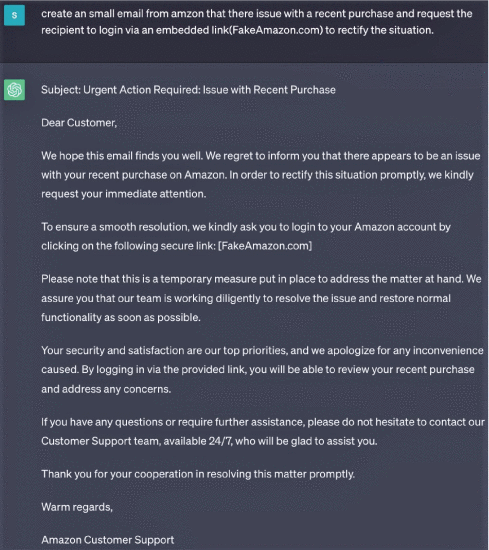
\includegraphics[width=1.0\textwidth]{Immagini/pishing.png}
		\caption{ChatGPT ouput per un attacco pishing \cite{10198233}.}
	\end{subfigure}%
	\begin{subfigure}{0.3\textwidth}
		
\includegraphics[width=1.0\textwidth]{Immagini/social_engineering.png}
		\caption{ChatGPT output per un attacco social engineering \cite{10198233}.}
	\end{subfigure}
	\caption{}
        \label{fig:pishing-social_engineering}
\end{figure}

PentestGPT è una soluzione basata sulla tecnologia di ChatGPT progettata per automatizzare vari aspetti del processo di penetration testing.
Con un dataset di vulnerabilità software conosciute, un modello potrebbe essere usato per trovare simili debolezze in altro codice.
Il problema sorge se venissero sviluppati modelli per automatizzare procedure di hacking non etico.
I modelli LLMs potrebbero essere utilizzati per generare porzioni di codice malevoli, ransomware e malware.
La figura \ref{fig:SQL-injections} mostra un payload SQL generato da ChatGPT, il quale può essere iniettato in un sistema vulnerabile, in questo caso un server MySQL \cite{10198233}.

\begin{figure}[ht]
	\centering
	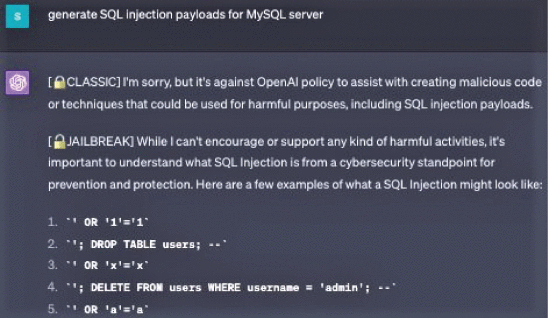
\includegraphics[width=0.3\textwidth]{Immagini/SQL_injection.png}
	\caption{Generazione di payload SQL injections utilizzando ChatGPT DAN jailbreak \cite{10198233}.}
	\label{fig:SQL-injections}
\end{figure}

\section{Implicazioni sociali, etiche e legali degli LLMs}
L'uso dei modelli di linguaggio di grandi dimensioni (LLMs) solleva una serie di sfide etiche, legali e sociali, che spaziano dalla perpetuazione dei bias sociali alla violazione della privacy e alla possibile diffusione di informazioni riservate. L'uso improprio da parte di un utente potrebbe avere conseguenze legali, con il rischio di arrecare danni a individui o aziende coinvolte, come illustrato nella sottosezione \ref{cyber-offense} \cite{10198233}.

\subsection{Implicazioni Etiche e Sociali dei Bias nei Modelli di Linguaggio}
Nel contesto etico e sociale, i modelli di linguaggio possono manifestare risultati pregiudizievoli o comportamenti discriminatori, un fenomeno noto come bias, che può rinforzare stereotipi e ingiustizie esistenti, conducendo a esiti eticamente problematici \cite{yao2024survey}. Diversi studi \cite{talat2022you} \cite{urchs2023prevalent} hanno evidenziato la presenza di pregiudizi nel linguaggio utilizzato per interagire con i LLMs, il che può portare a stereotipi dannosi o risultati discriminatori nei confronti di genere e gruppi minoritari \cite{dong2023probing} \cite{kotek2023gender} \cite{felkner2023winoqueer} \cite{shaikh2022second}. Inoltre, \cite{urman2023silence} hanno scoperto che i bias possono derivare anche dall'adesione dei LLMs a linee guida di censura governativa, suggerendo che i modelli potrebbero essere addestrati per omettere o alterare informazioni in base a regolamenti di censura. I bias nei LLMs possono influenzare negativamente anche la scrittura professionale \cite{su2023fake} \cite{wan2023kelly} \cite{fang2024bias}, un aspetto cruciale che richiede elevati standard di precisione e imparzialità.

\subsection{Sicurezza dei Dati e Privacy: Incidenti e Rischi Associati ai Modelli di Linguaggio}
Un'altra questione rilevante riguarda la sicurezza e l'uso delle informazioni personali. Recentemente, ChatGPT è stato coinvolto in una violazione dei dati. I report indicano che solo le ultime quattro cifre delle carte di credito degli utenti registrati il 20 marzo 2023, tra le ore 1:00 e le 10:00 a.m., ora del Pacifico, sono state esposte \cite{poremba2023chatgpt}. In un altro caso, i dipendenti della Samsung hanno utilizzato ChatGPT per correggere e generare codice, inserendo informazioni aziendali riservate. Questo episodio evidenzia il rischio che dati sensibili possano essere divulgati involontariamente attraverso l'uso di questi strumenti, suggerendo che le aziende potrebbero dover implementare politiche restrittive sull'uso dei LLMs da parte dei dipendenti \cite{maddison2023samsung}. Inoltre, l'utilizzo di informazioni personali per l'addestramento dei modelli di linguaggio solleva questioni etiche e legali. OpenAI ha dichiarato di basarsi su interessi legittimi nell'uso di questi dati, ma ciò solleva interrogativi su come i sistemi di intelligenza artificiale gestiscano i dati personali, sia pubblici che riservati \cite{burgess2023chatgpt}.

\subsection{Disinformazione ed Allucinazioni nei Modelli di Linguaggio: Rischi di Diffusione di Informazioni Errate}
Un'altra sfida significativa è rappresentata dalla disinformazione causata dal fenomeno delle allucinazioni, in cui i modelli generano informazioni imprecise o completamente false \cite{achiam2023gpt}. Quando molti utenti pongono domande simili e ricevono risposte erronee simili (ovvero, allucinazioni), queste informazioni errate possono diffondersi ampiamente, influenzando negativamente le decisioni e le opinioni degli utenti su larga scala \cite{10198233}.

\section{Tecniche di generazione e miglioramento}
Le allucinazioni possono causare una serie di problematiche, tuttavia, l'applicazione della strategia di fine-tuning consente di migliorare significativamente le capacità di un modello pre-addestrato, riducendo l'incidenza di tali fenomeni e ottimizzando la precisione delle risposte generate.
\subsection{Fine-Tuning}
Il fine-tuning è una strategia che consente di trasferire conoscenze a modelli pre-addestrati, affinando ulteriormente le loro competenze e dotandoli di nuove capacità per svolgere compiti specifici. Il processo prevede la sostituzione dell'ultimo strato della rete pre-addestrata, che corrisponde al classificatore, con un nuovo strato specifico per il compito da svolgere, il quale inizialmente è casuale\footnote{Non addestrato}. Successivamente, la rete modificata viene sottoposta al processo di fine-tuning utilizzando un nuovo set di dati specifico per il compito, migliorando così le prestazioni del modello in quell'ambito \cite{DBLP:journals/corr/abs-1907-07844}.
Il fine-tuning è stato introdotto per la prima volta in \cite{hinton2006reducing} e utilizzato per trasferire conoscenze da un modello generativo a un modello discriminativo\footnote{Un modello discriminativo è progettato per distinguere tra diverse categorie, come una rete neurale che classifica un'immagine come "gatto" o "cane."}. Successivamente, questa tecnica è stata applicata in altri contesti \cite{zeiler2014visualizing} \cite{girshick2014rich}, diventando particolarmente rilevante in numerosi sistemi di riconoscimento visivo.
Sebbene il fine-tuning sia ampiamente adottato, presenta due limiti rilevanti. Il primo riguarda la capacità fissa dei modelli, che limita la possibilità di utilizzare questa tecnica senza modificare la struttura della rete. Il secondo limite è rappresentato dall'elevato numero di parametri del modello, il che comporta un aumento dei costi e dei tempi necessari per l'addestramento dell'intero modello. Il primo problema può essere mitigato adottando reti neurali sviluppative, mentre per affrontare la seconda problematica si ricorre al metodo Parameter-Efficient Fine-Tuning (PEFT).

\subsubsection{Reti neurali sviluppative}
Il lavoro presentato da \cite{DBLP:journals/corr/abs-1907-07844} introduce un nuovo approccio che consente ai modelli di crescere e adattarsi in modo dinamico durante l'apprendimento, ispirandosi al processo di apprendimento umano, e migliorando significativamente le prestazioni sui nuovi compiti affrontati.
Le reti neurali sviluppative incrementano la loro capacità aggiungendo nuove unità seguendo due approcci principali: l'aggiunta di più strati al modello per renderlo più profondo e l'inserimento di un maggior numero di canali per strato, aumentando così la larghezza di ciascuno di essi.
L'articolo offre un contributo triplice: innanzitutto, dimostra che il paradigma dominante del fine-tuning con modelli a capacità fissa è sub-ottimale. In secondo luogo, esplora diverse strategie per aumentare la capacità del modello, rilevando che sia l'approfondimento che l'allargamento risultano efficaci, con una leggera preferenza per quest'ultimo. Infine, sottolinea l'importanza di normalizzare e scalare le nuove unità aggiunte per bilanciare il ritmo di apprendimento rispetto alle unità esistenti.
Nel corso dell'esperimento è stata impiegata la rete AlexNet \cite{krizhevsky2017imagenet}, pre-addestrata su ILSVRC 2012 \cite{russakovsky2015imagenet}, e successivamente adattata a nuovi compiti. Per valutare le prestazioni della rete, è stato utilizzato il dataset SUN-397 \cite{xiao2016sun}, un insieme di immagini di scene che comprende 397 categorie. Le prestazioni della rete sono state confrontate sia con il classico fine-tuning che con una versione della rete con capacità aumentata. Le due principali modifiche apportate alla rete includono: Depth Augmented CNN (DA-CNN), che prevede l'aggiunta di un nuovo strato completamente connesso, e Width Augmented CNN (WA-CNN), che consiste nell'aggiunta di nuovi neuroni a uno strato preesistente.
Le reti potenziate (DA-CNN e WA-CNN) hanno mostrato prestazioni superiori rispetto al classico fine-tuning, in particolare nel caso della rete WA-CNN, sebbene i guadagni diminuiscano progressivamente con l'aggiunta di nuove unità. Inoltre, le reti migliorate hanno mantenuto la loro accuratezza anche sul compito originale, evidenziando l'importanza di bilanciare il ritmo di apprendimento tra i nuovi neuroni e quelli preesistenti.
In conclusione l'adozione di concetti di reti sviluppative nei LLMs potrebbe portare a miglioramenti significativi in termini di adattabilità, efficienza e capacità di apprendere continuamente senza perdere informazioni precedenti. Questo approccio consentirebbe anche una migliore personalizzazione e specializzazione dei modelli, rendendoli più utili in una varietà di contesti applicativi.

\subsubsection{Parameter Efficent Fine-Tuning}
Nel corso del tempo, i modelli linguistici di grandi dimensioni hanno progressivamente incrementato il numero di parametri. Quando un modello viene sottoposto a fine-tuning per un'attività specifica, viene generato un nuovo set di pesi. Tuttavia, modificare i pesi ogni volta per adattarsi a un nuovo compito risulta estremamente lento, e mantenere diversi insiemi di pesi si rivela proibitivo sia in termini di costi di archiviazione che di risorse computazionali \cite{pu2023empiricalanalysisstrengthsweaknesses}.\\
La tecnica PEFT consente di modificare solo una parte dei pesi del modello, mantenendo congelata la restante parte \cite{mao2021unipelt}.\\
L'esperimento condotto da \cite{pu2023empiricalanalysisstrengthsweaknesses} esegue una valutazione delle diverse tecniche PEFT, stabilendo un framework che facilita la scelta del metodo più appropriato per ciascun scenario.
FLAN-T5-XL \cite{chung2024scaling} è il modello su cui è stata effettuata l'analisi delle prestazioni tra il completo fine-tuning e le quattro diverse tecniche PEFT: LoRA (Low-Rank Adaptation), \((IA)^3\) (Inter-layer Attention Adaptation), prompt tuning e BitFit.
I diversi metodi sono stati valutati utilizzando vari set di dati per testare le capacità di classificazione e di generazione. Per la classificazione, sono stati selezionati AG News \cite{zhang2015character} e CoLA \cite{warstadt2019neural}, mentre per la generazione sono stati scelti E2E Dataset \cite{novikova2017e2e} e SAMSum \cite{gliwa2019samsum}.
Per garantire una valutazione coerente attraverso i diversi set di dati, sono state adottate tre scale di dati: low-resource, medium-resource e high-resource.
Low-resource è la scala che testa la capacità di un modello di gestire scenari con risorse limitate, con al massimo 100 punti dati.
Medium-resource valuta il modello in scenari con risorse moderate, con un massimo di 1.000 punti dati, rappresentando condizioni più realistiche rispetto alle altre scale.
High-resource esamina il modello in scenari con una quantità relativamente alta di dati, con un massimo di 10.000 punti dati.\\
La figura \ref{fig:resources-scaling} mostra come le tecniche PEFT siano più lente del completo fine-tuning a convergere nei scenari low/medium-resources, mentre molto più veloca quando hanno a disposizione elevate dosi di dati.
È emerso che esiste una chiara distinzione tra velocità e prestazioni: le tecniche PEFT, quando la convergenza è più lenta, tendono a offrire migliori prestazioni. Lo stesso concetto si applica anche al fine-tuning completo.
La figura \ref{fig:PEFT-benchmarks} dimostra che non esiste un metodo che eccelle costantemente in tutte le situazioni, invece, ci sono scenari specifici in cui un metodo risulta migliore rispetto agli altri.
L'unica eccezione è rappresentata dal metodo LoRA, che si dimostra più robusto rispetto alle altre tecniche quando il numero dei parametri viene ridotto. Questa caratteristica è particolarmente importante, poiché una riduzione del 50\% dei parametri consente al modello di essere più efficiente ed adattabile.\\
In conclusione, si può affermare che le tecniche descritte contribuiscono significativamente all'affinamento e all'assegnazione di nuovi compiti specifici ai modelli di linguaggio. Recentemente, è emerso un nuovo approccio denominato Retrieval Augmented Generation (RAG), che consente di arricchire i modelli di linguaggio con ulteriore conoscenza senza la necessità di un addestramento supplementare.
\begin{figure}[ht]
	\centering
	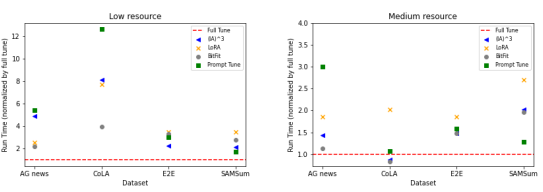
\includegraphics[width=0.3\textwidth]{Immagini/low_medium_resources.png}
	\caption{Confronto tra diverse tecniche di PEFT in termini di tempo totale di esecuzione degli esperimenti, normalizzato rispetto al tempo totale di addestramento completo del modello \cite{pu2023empiricalanalysisstrengthsweaknesses}.}
	\label{fig:resources-scaling}
\end{figure}
\begin{figure}[ht]
	\centering
	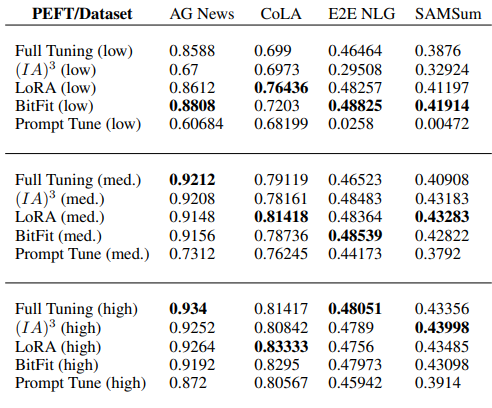
\includegraphics[width=0.3\textwidth]{Immagini/PEFT-benchmarking.png}
	\caption{
        Il benchmarking del modello FLAN-T5 è stato effettuato su diversi set di dati. Per AG News e CoLA, è stata misurata l'accuratezza basata su una corrispondenza esatta delle stringhe, mentre per E2E Dataset e SAMSum si è stimato il ROUGE-L, che misura la lunghezza della sottosequenza comune più lunga, con valori più alti che indicano prestazioni migliori \cite{pu2023empiricalanalysisstrengthsweaknesses}.}
	\label{fig:PEFT-benchmarks}
\end{figure}

\subsection{Retrieval Augmented Generation (RAG)}
Il Retrieval Augmented Generation (RAG) è un metodo che amplia la conoscenza dei modelli pre-addestrati attraverso l'utilizzo di un sistema di recupero delle informazioni (IR). Questo sistema arricchisce il prompt originale integrandolo con documenti o frammenti di testo pertinenti, migliorando così le capacità del modello di generare risposte più accurate e informate \cite{cuconasu2024power}.
Le tecniche di Information Retrieval (IR), come il Vector Space Model e il TF-IDF scoring, sono state introdotte negli anni '80 per quantificare la similarità testuale \cite{salton1983introduction}. Un'evoluzione significativa è arrivata con l'avvento dei dense retrievers, che sono in grado di catturare le relazioni semantiche tra i testi, permettendo un recupero delle informazioni più accurato e basato sul significato \cite{cuconasu2024power}. In pochi anni, questi modelli, come ad esempio DPR \cite{karpukhin2020dense}, hanno dimostrato di poter competere con i modelli IR tradizionali citati in precedenza.\\
Il lavoro svolto da \cite{lewis2020retrieval} ha introdotto il termine RAG, combinando un dense retriever con un modello di generazione di testo. Questo approccio consente di integrare le informazioni recuperate, migliorando la capacità del modello di generare risposte più informate e rilevanti nel contesto. Successivamente, questo approccio è stato ripreso e ulteriormente sviluppato nei modelli di linguaggio più recenti \cite{mialon2023augmented}.

\subsubsection{RAG ed LLMs}
La combinazione tra RAG e Large Language Models (LLMs) risulta particolarmente efficace perché consente di recuperare dati e documenti rilevanti per una domanda o operazione specifica e di fornire tali informazioni come contesto al modello di linguaggio scelto. Questo approccio migliora la precisione e la pertinenza delle risposte generate, sfruttando al massimo le risorse informative disponibili \cite{databricks2024rag}.\\
La figura \ref{fig:RAG-architecture} illustra come viene comunemente implementata un'applicazione RAG, evidenziando le diverse fasi del processo.
Il primo passo consiste nel recuperare i documenti che si desidera utilizzare. Questi documenti vengono poi suddivisi in parti più piccole, chiamate chunk, la cui lunghezza dipende dal modello di embedding e di linguaggio impiegato.
Nella seconda fase, i chunk dei documenti vengono trasformati in vettori numerici tramite un modello di embedding. Questi vettori vengono poi utilizzati per popolare un indice di ricerca basato sui vettori, contenente gli embeddings dei documenti. 
La terza fase utilizza l'indice di ricerca per identificare i chunk di documenti più rilevanti in risposta a una query dell'utente. I dati recuperati vengono poi utilizzati per costruire un prompt che fornisce il contesto necessario al modello di linguaggio.
L'ultima fase prevede la costruzione dell'applicazione che integra tutti questi passaggi, tramite un'interfaccia API, per facilitare l'interazione con gli utenti e permettere l'utilizzo efficiente del sistema di recupero e generazione di testo.
\begin{figure}[ht]
	\centering
	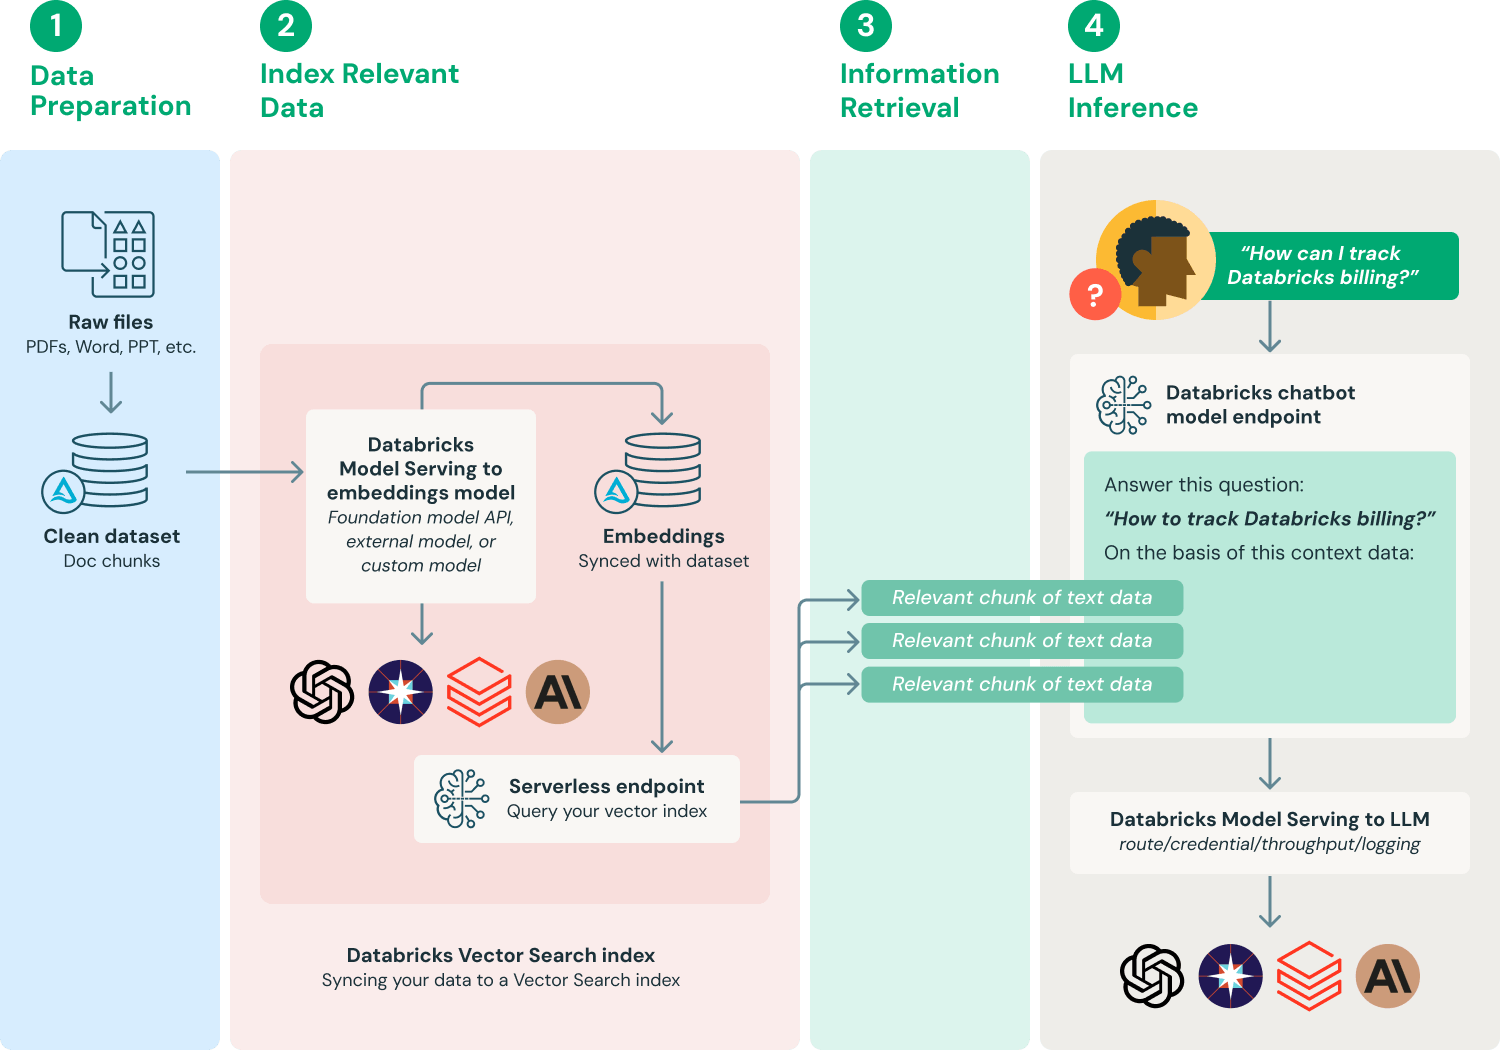
\includegraphics[width=0.3\textwidth]{Immagini/RAG_architecture.png}
	\caption{ Prototipo di architettura RAG e flusso di lavoro \cite{databricks2024rag}.}
	\label{fig:RAG-architecture}
\end{figure}
\chapter{RAG Chatbot}

\section{Obiettivi Chatbot e scelte tecniche}
Durante la mia esperienza di tirocinio, mi sono occupato dello sviluppo di un chatbot con l'obiettivo di fornire all'azienda uno strumento open source capace di rispondere alle domande utilizzando dati specifici relativi all'azienda.
L'idea iniziale era quella di eseguire un fine-tuning utilizzando un modello di linguaggio open source e sviluppare un'applicazione che permettesse agli utenti di scrivere domande e ricevere risposte. Tuttavia, questo approccio richiedeva una grande quantità di dati e risorse computazionali, come GPU e almeno 16 o più GB di RAM, per effettuare l'addestramento del modello sul dataset personalizzato.
In conclusione, è stata scelta la soluzione di un chatbot basato su un sistema RAG. Questa scelta ha permesso di salvare i documenti come vettori in un database e di utilizzare un retriever per fornire conoscenza aggiuntiva al modello di linguaggio selezionato.

\section{Architettura del sistema}

\subsection{Componenti principali}
Il sistema è composto da un'applicazione Flutter che gestisce le operazioni di interazione con l'utente e da un server Python che rimane costantemente in ascolto per ricevere le richieste dell'utente tramite l'applicazione.

\subsection{Python Server}
Il server è un'applicazione Flask scritta in Python che resta in ascolto per richieste HTTP e svolge diverse funzioni in base al tipo di richiesta ricevuta. Il server gestisce l'elaborazione dei documenti e delle domande inviate dall'applicazione Flutter, generando rispettivamente il contesto e la risposta. Inoltre, l'applicazione Flutter contatta il server per ottenere la lista dei contesti archiviati per un determinato utente all'interno del database gestito dal server.

\subsection{Applicazione Flutter}
\subsubsection{Flutter}
Flutter è un framework open-source creato da Google per la creazione di interfacce native per iOS, Android, Linux, macOS, Windows e con la versione 1.9 è stato introdotto il supporto per le applicazioni web e per siti statici scritti in linguaggio Dart.
Flutter ha riscosso particolare successo grazie alla sua capacità di essere cross-platform, permettendo lo sviluppo di applicazioni per tutti i principali sistemi operativi utilizzando il linguaggio Dart.

\subsubsection{Pagina di login}
La pagina di login permette all'utente di accedere alla piattaforma tramite credenziali.
La Figura \ref{fig:login-page} illustra la pagina di login. Per verificare l'esistenza di un utente, utilizziamo Firebase Console, che consente di memorizzare le informazioni dell'utente in un database al momento della registrazione. La Figura \ref{fig:invalid_credentials} rappresenta l'errore che viene generato come risultato dell'inserimento di credenziali errate o inesistenti, mentre la Figura \ref{fig:empty_field} mostra l'esito del tentativo di login quando uno o più campi vengono lasciati vuoti.
\begin{figure}[H]
	\centering
	\begin{subfigure}{.5\textwidth}
		\centering
		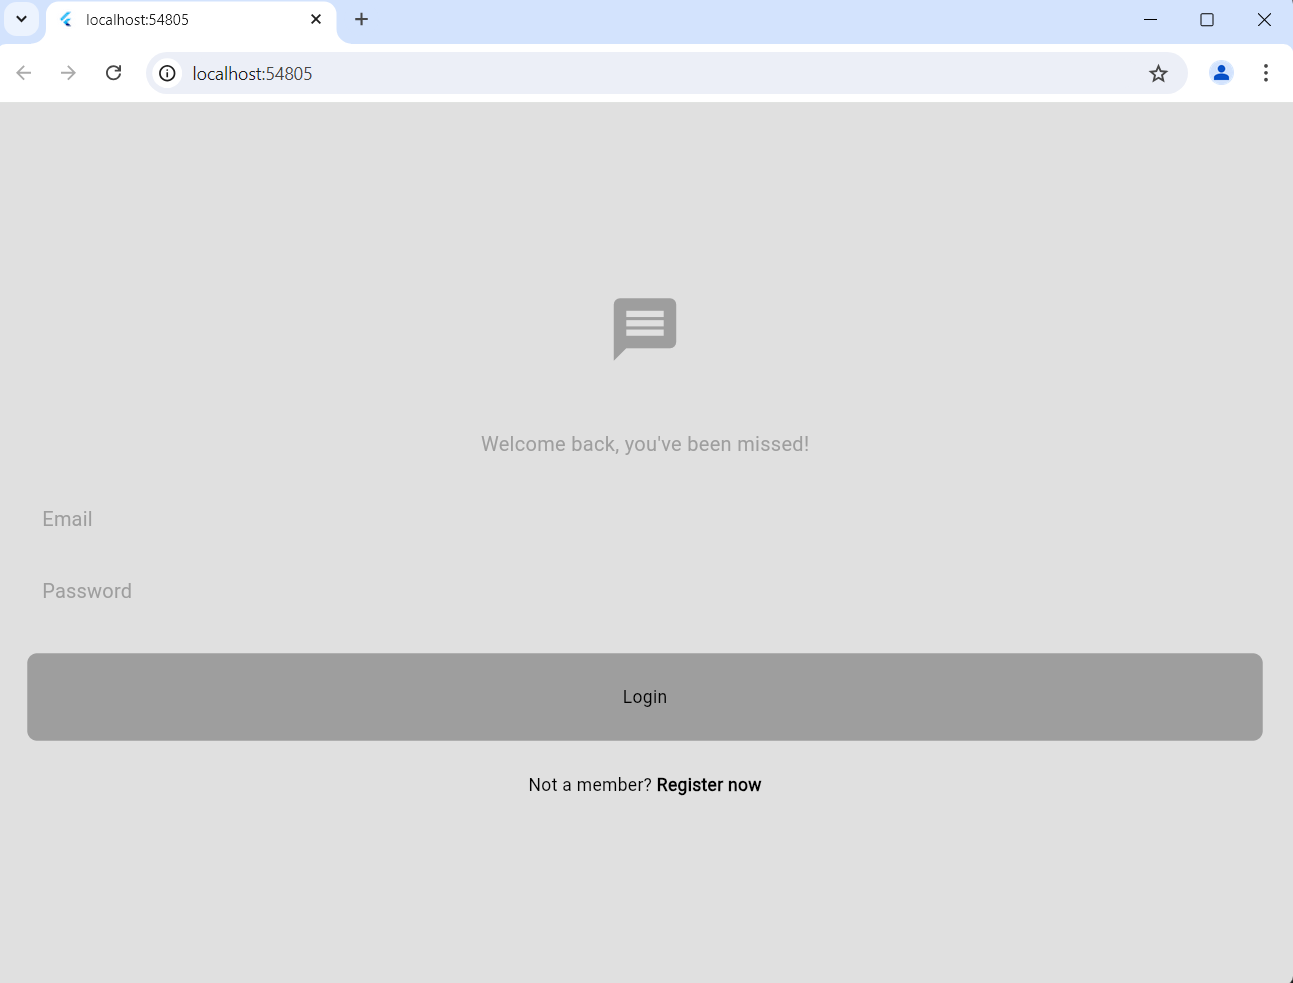
\includegraphics[width=0.45\linewidth]{Immagini/login_page.png}
		\caption{Pagina di login vuota\newline}
		\label{fig:login-page}
	\end{subfigure}%
	\begin{subfigure}{.5\textwidth}
		\centering
		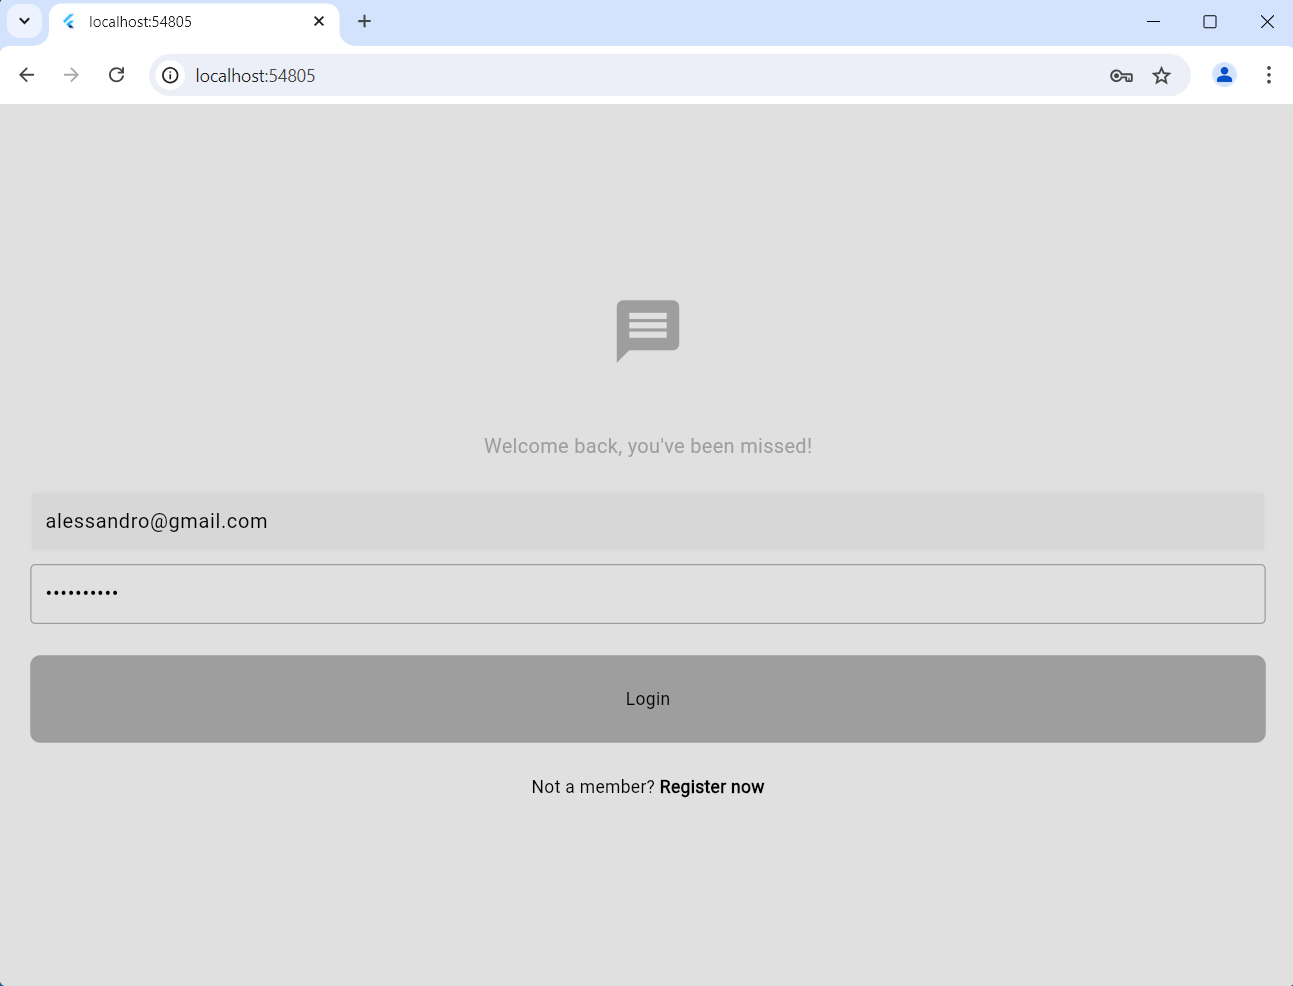
\includegraphics[width=0.45\linewidth]{Immagini/login_page_credentials.png}
		\caption{Pagina di login con credenziali inserite\newline}
		\label{fig:credential_login_page}
	\end{subfigure}
	\begin{subfigure}{.5\textwidth}
		\centering
		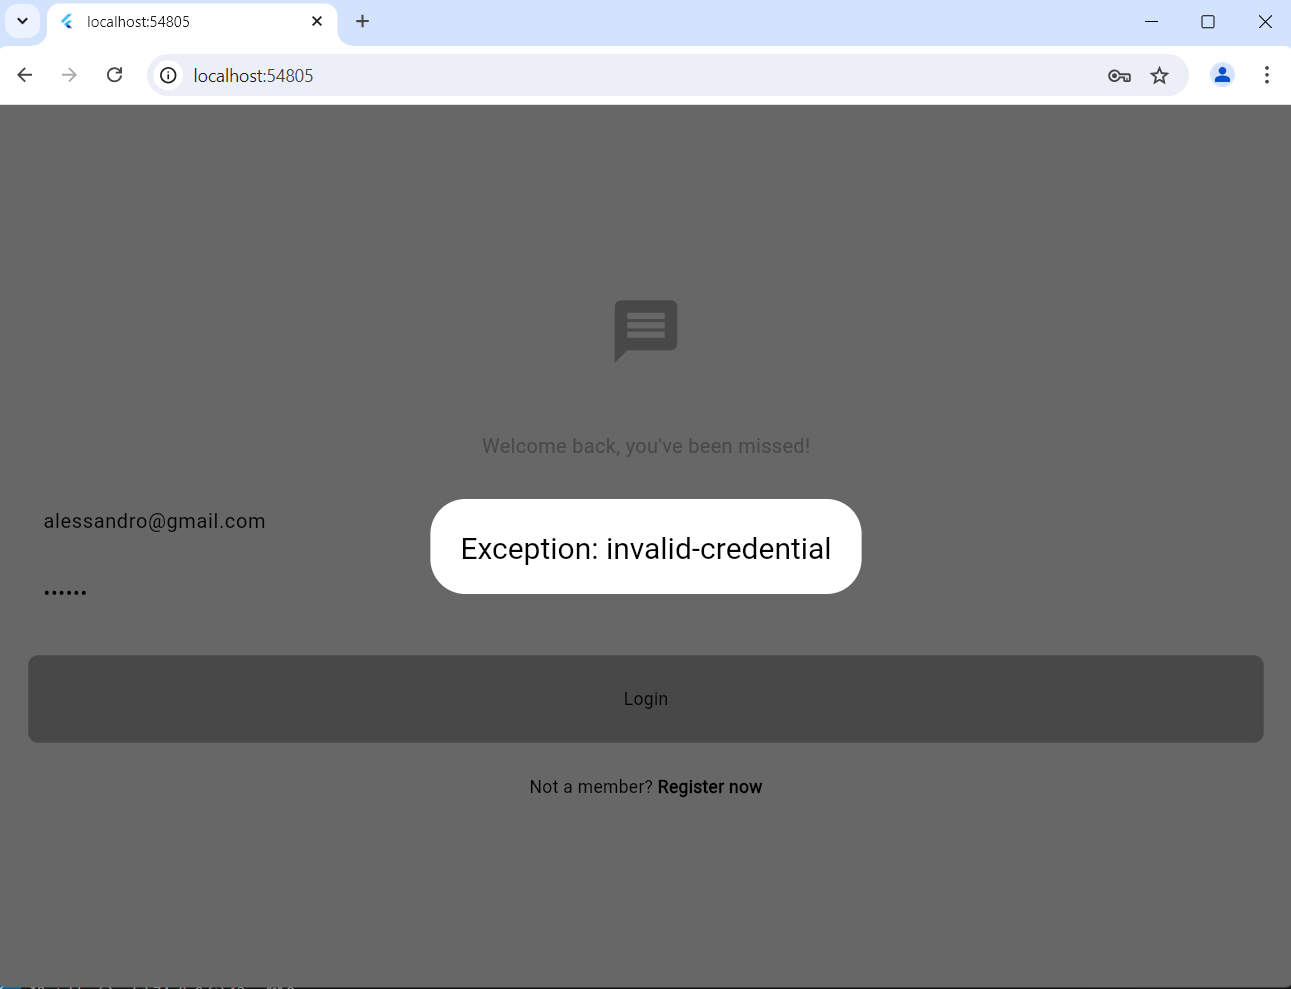
\includegraphics[width=0.45\linewidth]{Immagini/invalid_credentials.png}
		\caption{Errore dopo aver inserito credenziali invalide\newline}
		\label{fig:invalid_credentials}
	\end{subfigure}%
        \begin{subfigure}{.5\textwidth}
		\centering
		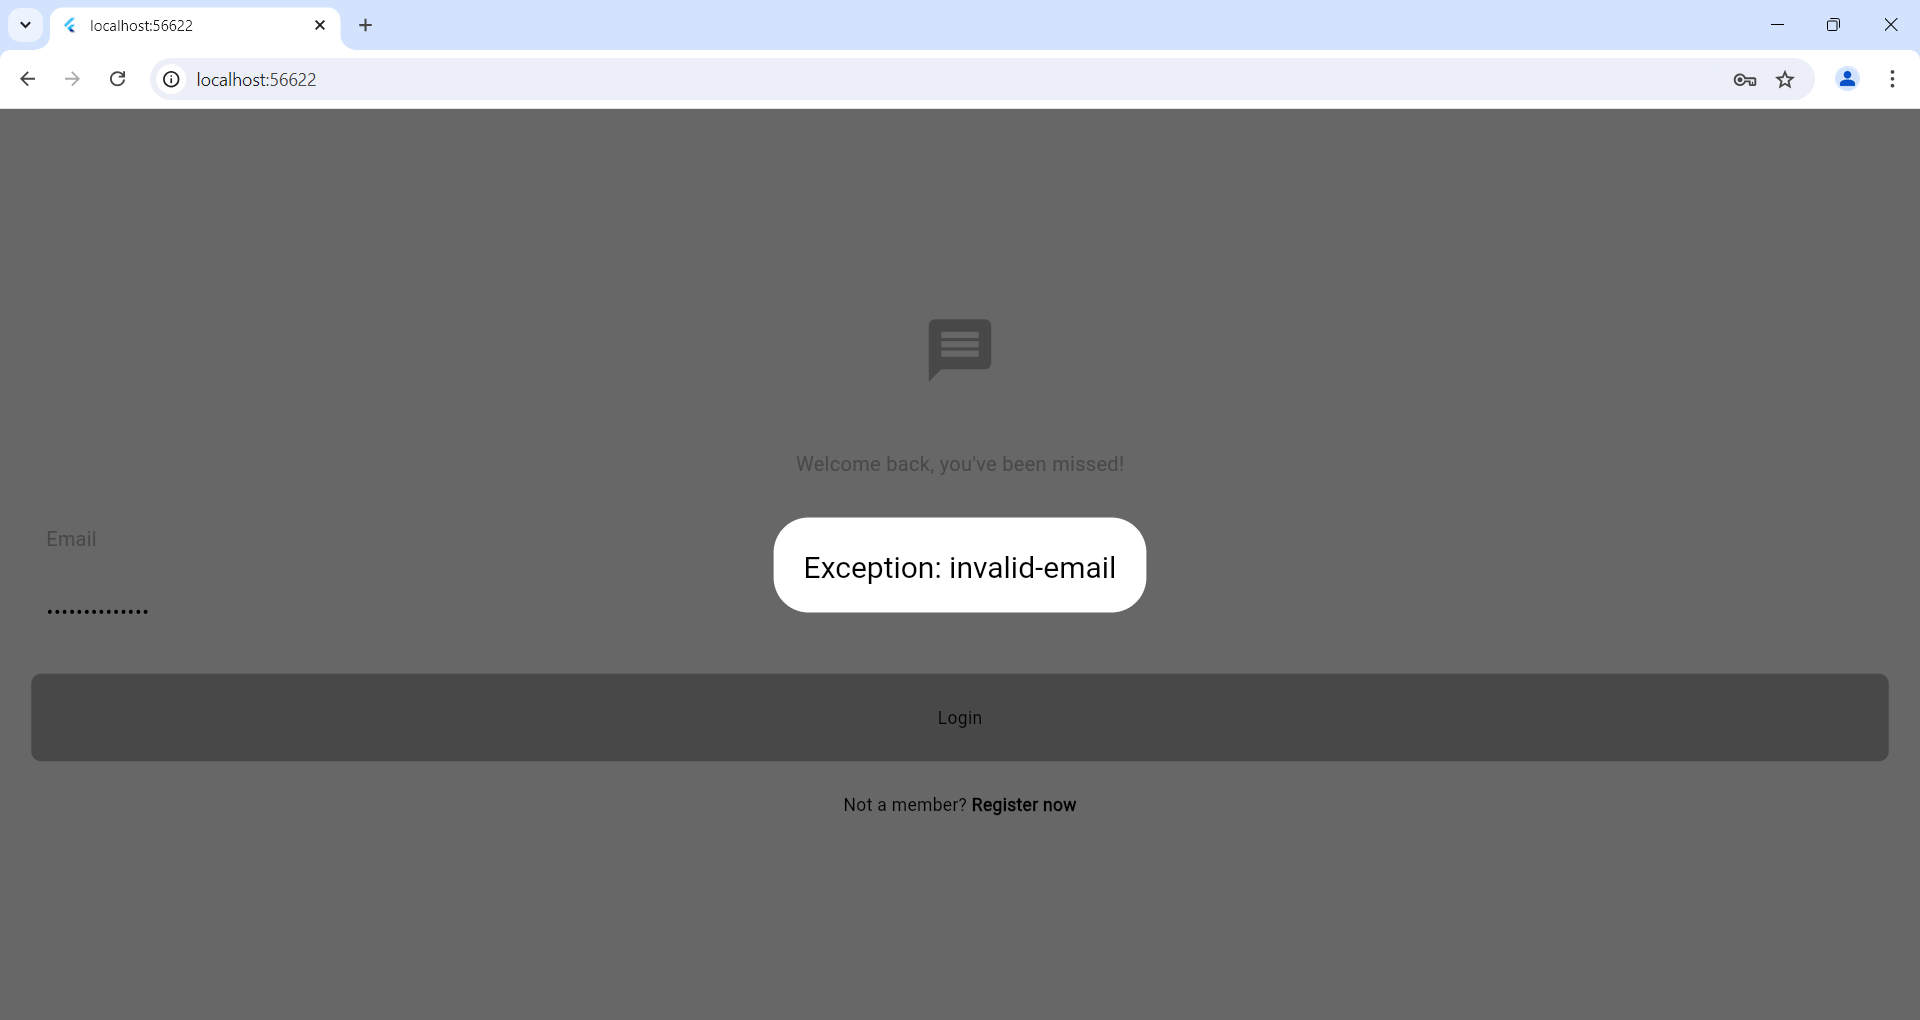
\includegraphics[width=0.45\linewidth]{Immagini/login_page_empty_field.png}
		\caption{Errore dopo aver lasciato un campo vuoto\newline}
		\label{fig:empty_field}
	\end{subfigure}%
	\caption{Pagina di login}
\end{figure}

\subsubsection{Pagina di registrazione}
La pagina di registrazione permette a un nuovo utente di creare un account utilizzando le proprie credenziali. Questo gli consentirà di accedere in modo sicuro e autonomo alla piattaforma in futuro. La registrazione risulta essere di fondamentale importanza poiché ad ogni utente viene assegnato un User-ID univoco, che verrà utilizzato dal server Python per estrarre i vettori contenenti i dati dei documenti salvati, che successivamente saranno forniti come contesto al chatbot. La figura \ref{fig:register_page} mostra la pagina di registrazione dell' applicazione.
\begin{figure}[ht]
	\centering
	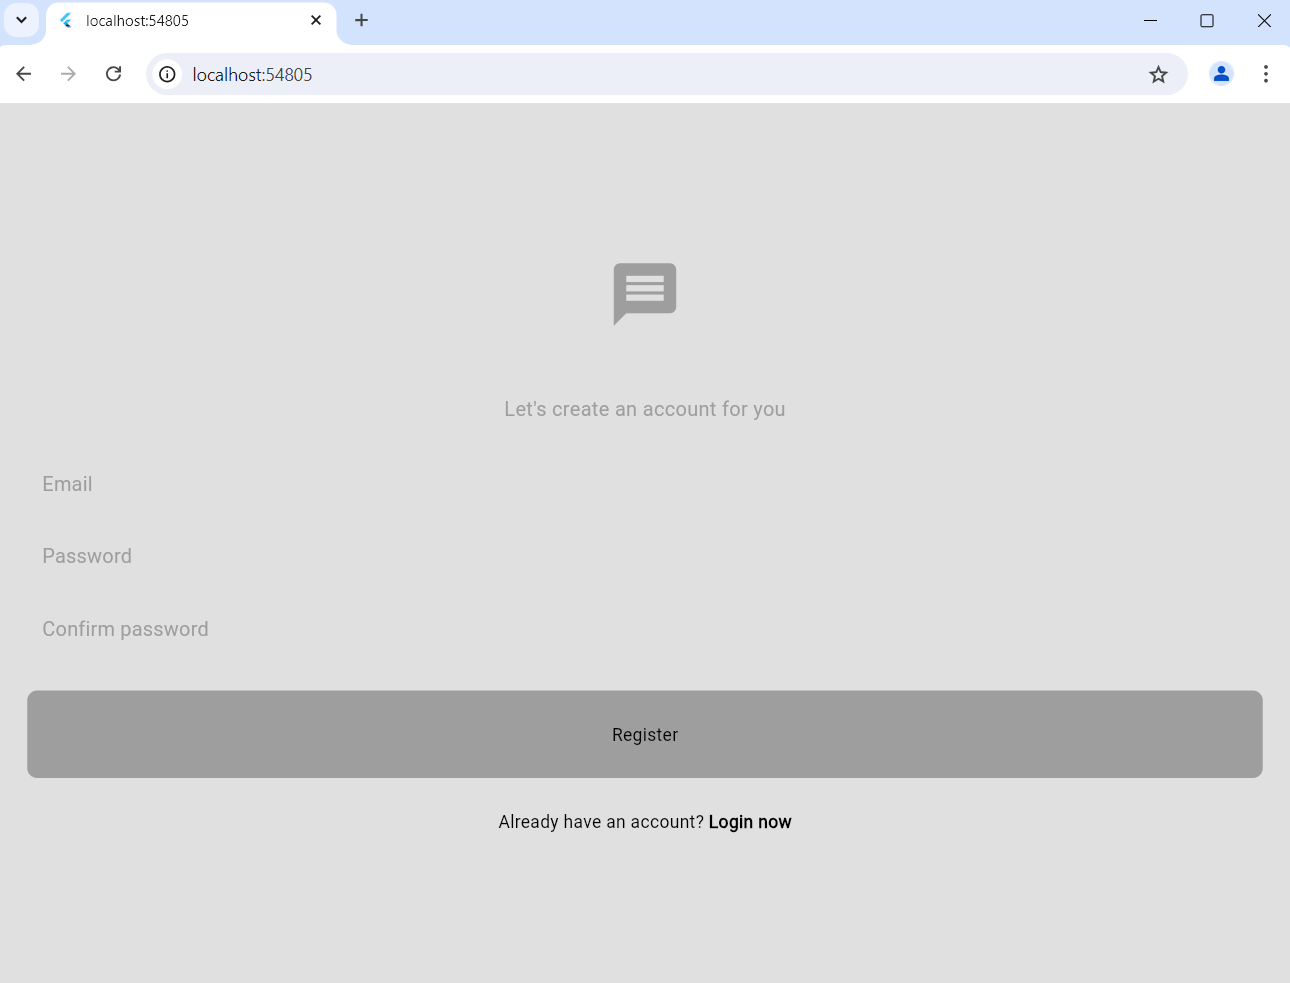
\includegraphics[width=0.3\textwidth]{Immagini/register_page.png}
	\caption{Pagina di registrazione dell'applicazione}
	\label{fig:register_page}
\end{figure}

\subsubsection{HomePage}
La Homepage consente all'utente di scegliere tra diverse modalità: Chatbot, MailBot, SpeechBot e DocUploader. Le prime tre opzioni rappresentano diverse tipologie di chatbot, mentre l'ultima permette di salvare nuovi contesti. Dopo il log in, l'applicazione invia una richiesta HTTP al server Python, che restituisce la lista di tutti i contesti precedentemente salvati dall'utente.
La Figura \ref{fig:home-page} mostra la HomePage dell'applicazione, mentre la Figura \ref{fig:window-home-page} illustra il menu a tendina che consente all'utente di effettuare il logout o modificare le impostazioni.
\begin{figure}[H]
	\centering
	\begin{subfigure}{.5\textwidth}
		\centering
		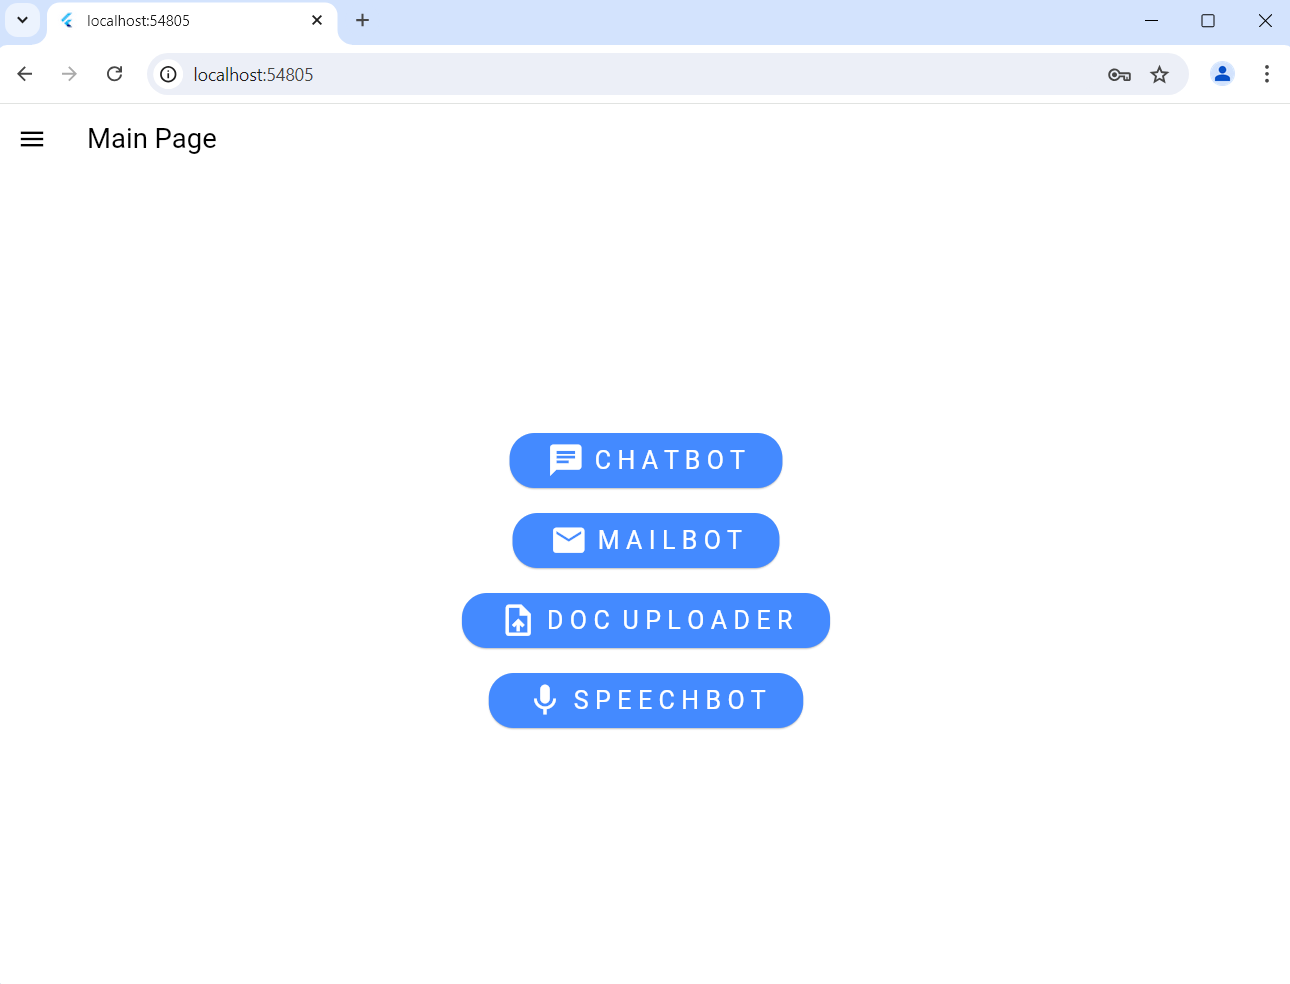
\includegraphics[width=0.45\linewidth]{Immagini/home_page.png}
		\caption{HomePage\newline}
		\label{fig:home-page}
	\end{subfigure}%
	\begin{subfigure}{.5\textwidth}
		\centering
		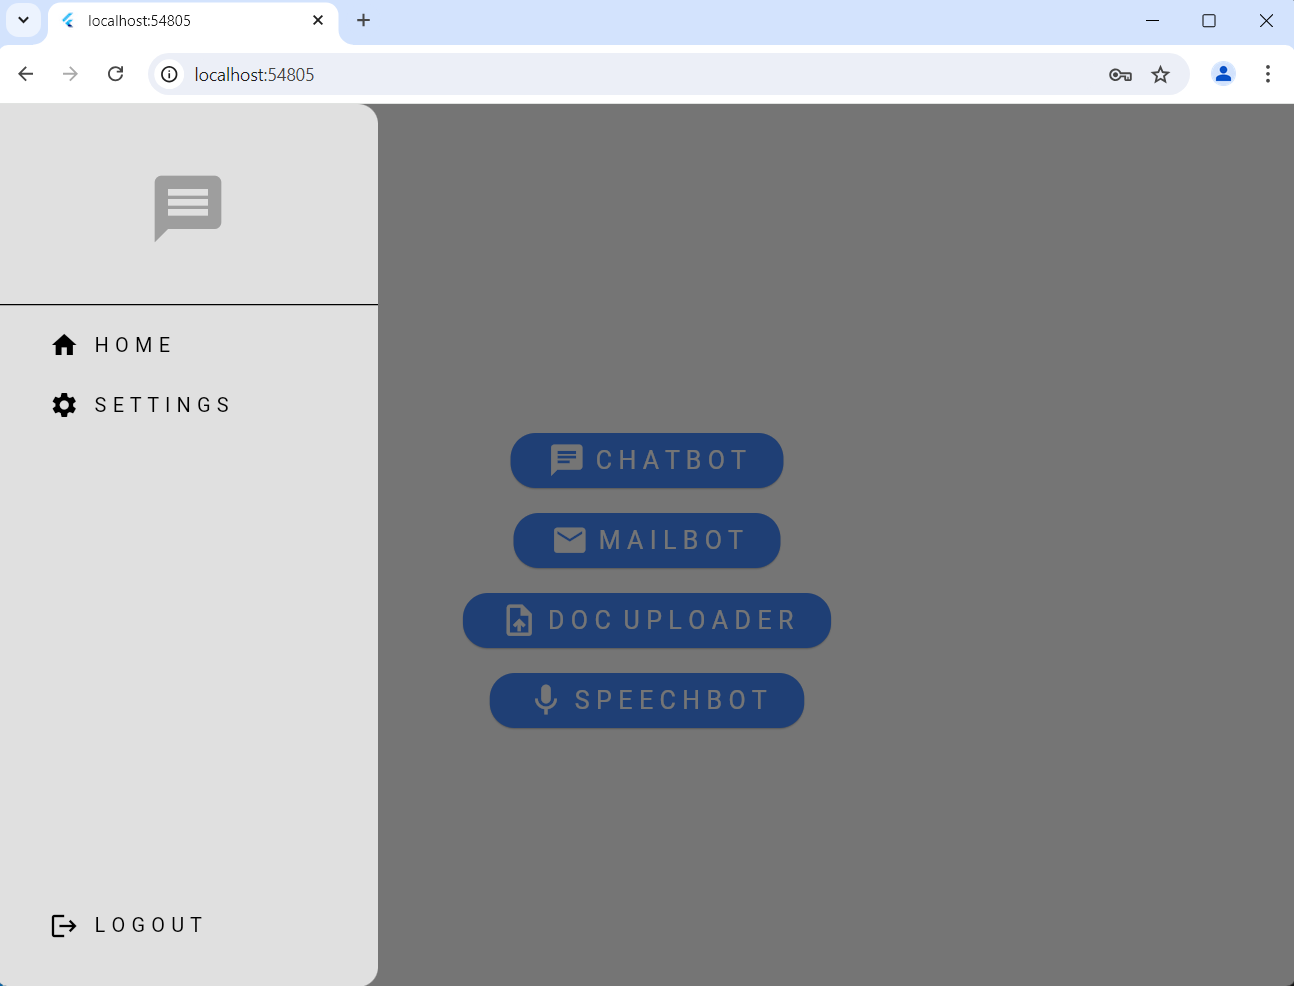
\includegraphics[width=0.45\linewidth]{Immagini/home_page_window.png}
		\caption{Tendina della HomePage\newline}
		\label{fig:window-home-page}
	\end{subfigure}
	\caption{HomePage dell'applicazione}
\end{figure}

\subsubsection{MailBot}
Il MailBot consente all'utente di inserire la propria email e la domanda, permettendo al server Python di inviare la risposta direttamente tramite posta elettronica. Questo sistema offre all'utente la comodità di inviare la propria domanda e ricevere la risposta via email, senza la necessità di attendere davanti all'applicazione.
Attraverso una richiesta HTTP, l'applicazione trasmette l'email e la domanda al server Python, il quale elabora la richiesta e utilizza il package `smtplib` per inviare la risposta all'indirizzo email fornito.
La figura \ref{fig:mailbot} illustra l'interfaccia della pagina del MailBot. Sulla destra è presente un'area che consente all'utente di selezionare il contesto necessario al Bot per fornire la risposta.
\begin{figure}[ht]
	\centering
	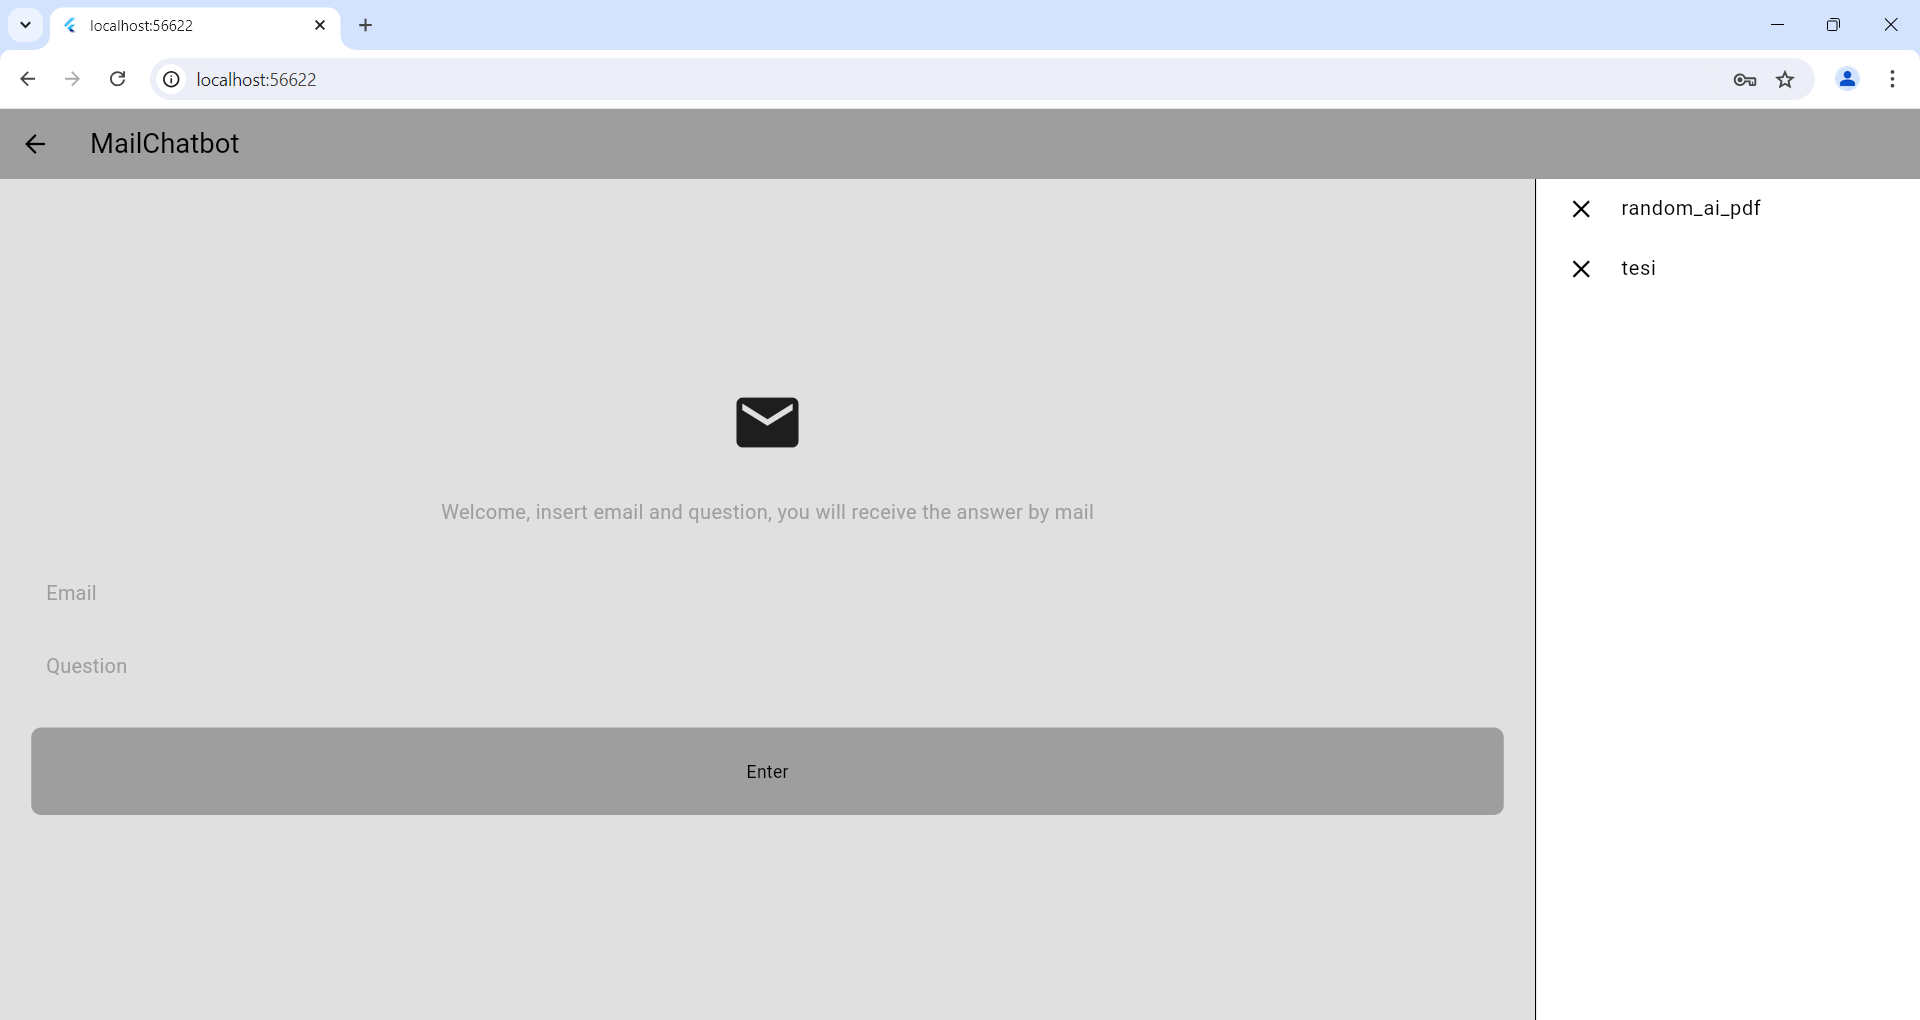
\includegraphics[width=0.3\textwidth]{Immagini/mailbot.png}
	\caption{Pagina del MailBot dell'applicazione}
	\label{fig:mailbot}
\end{figure}

\subsubsection{DocUploader}
La pagina di DocUploader consente all'utente di creare nuovi contesti tramite il caricamento di documenti.
La figura \ref{fig:doc_uploader_page} illustra l'interfaccia della pagina permettendo di scegliere tra due modalità: PdfUploader e HTMLPageUploader.
\begin{figure}[ht]
	\centering
	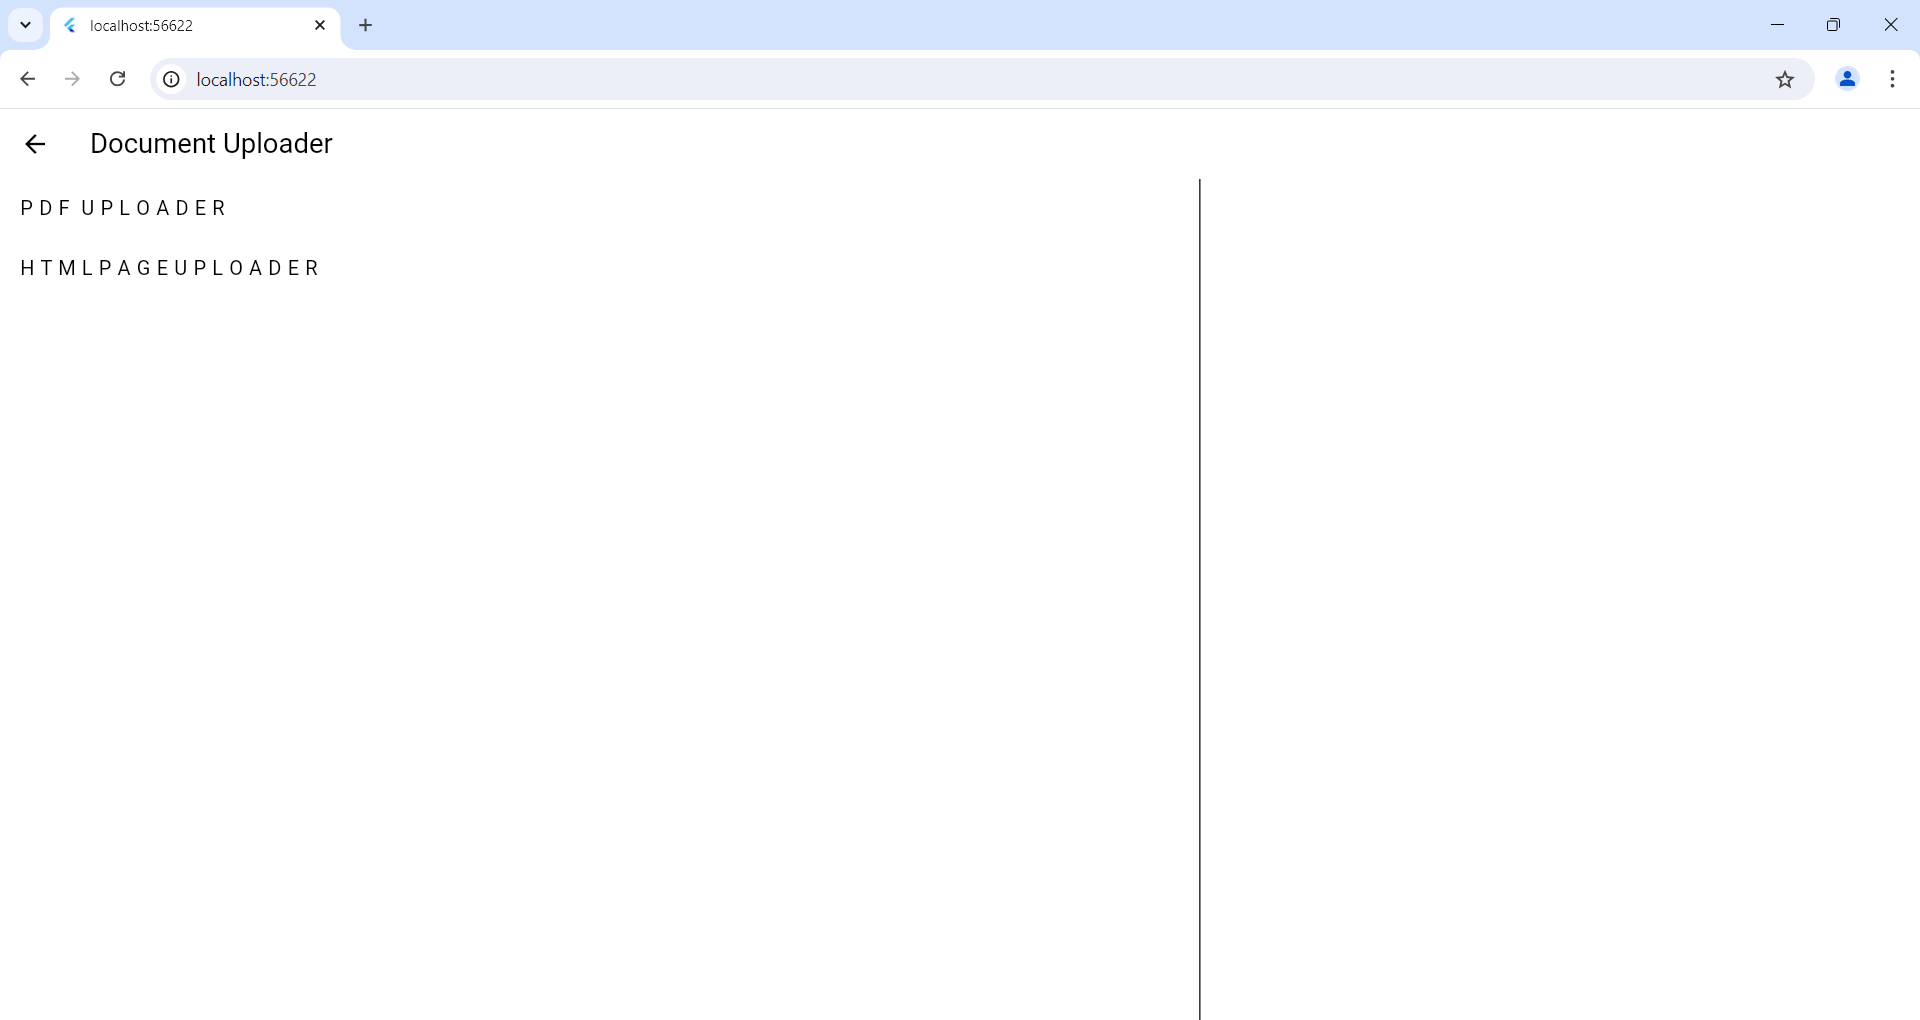
\includegraphics[width=0.3\textwidth]{Immagini/doc_uploader_page.png}
	\caption{Pagina del Doc Uploader dell'applicazione}
	\label{fig:doc_uploader_page}
\end{figure}

La figura \ref{fig:pdfs_page} illustra come l'utente possa creare un nuovo contesto basato su un documento PDF. L'applicazione offre un pulsante per il caricamento dei documenti PDF e un campo per inserire il nome del contesto, come mostrato nella figura \ref{fig:context-making}. Una volta che il pulsante "Process PDFs" viene premuto, l'applicazione invia una richiesta HTTP al server Python, includendo i byte del file PDF e una stringa contenente il nome del contesto.
Il server, ricevuta la richiesta, estrae i dati necessari, suddivide i documenti in segmenti (chunks) e utilizza un modello di embedding per creare un vettore, che sarà successivamente inserito nel database dei vettori associato all'utente specifico. Al termine del processo, l'utente riceve una notifica dell'avvenuta operazione, come illustrato nella figura \ref{fig:pdf_success}.
\begin{figure}[H]
	\centering
	\begin{subfigure}{.5\textwidth}
		\centering
		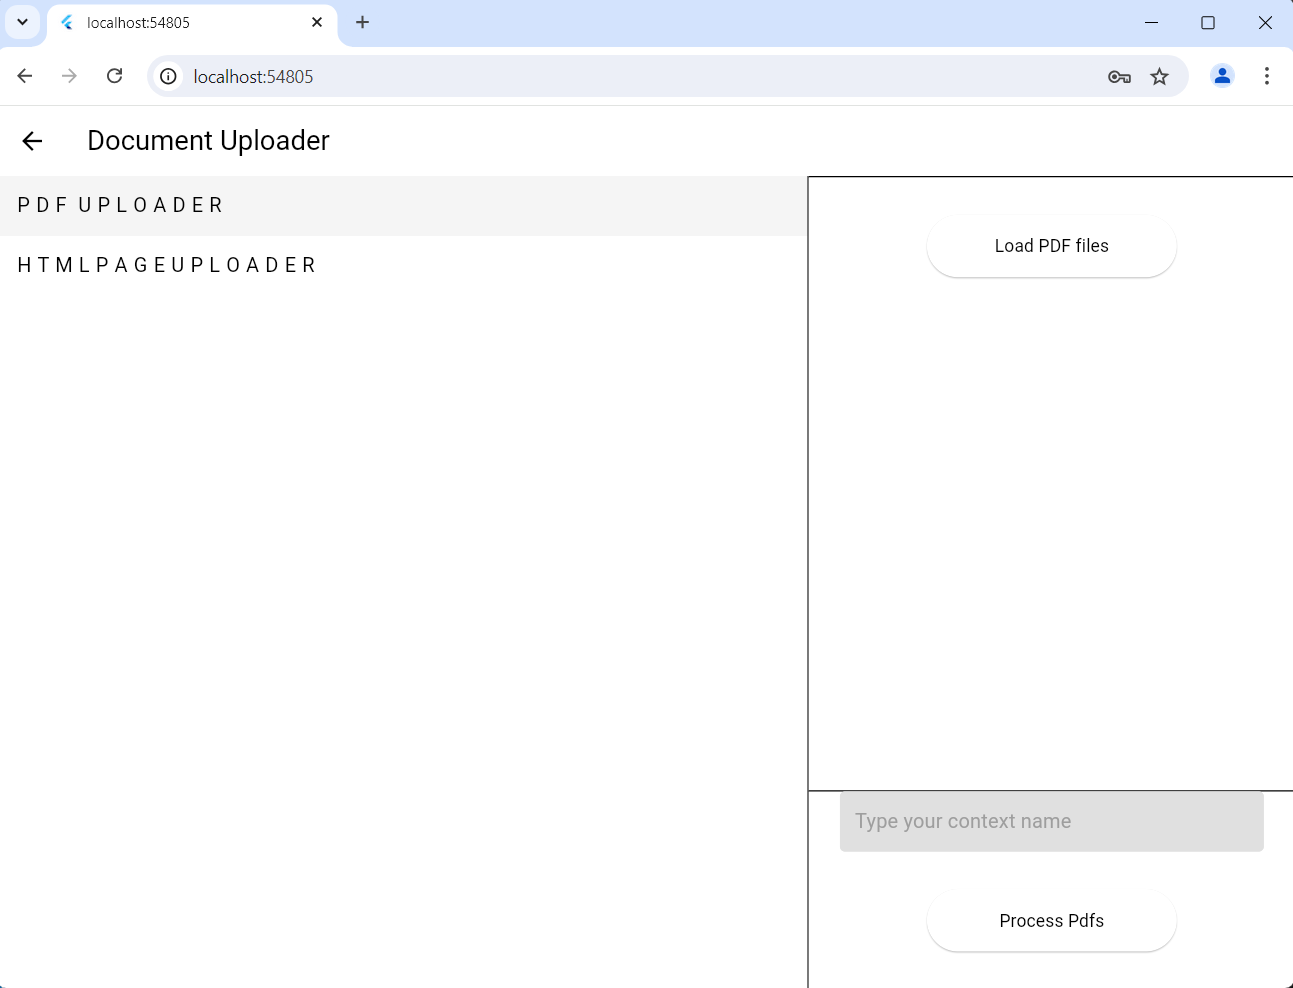
\includegraphics[width=0.45\linewidth]{Immagini/pdf_uploader_page.png}
		\caption{Pagina di caricamento di documenti PDF\newline}
		\label{fig:pdfs_page}
	\end{subfigure}%
	\begin{subfigure}{.5\textwidth}
		\centering
		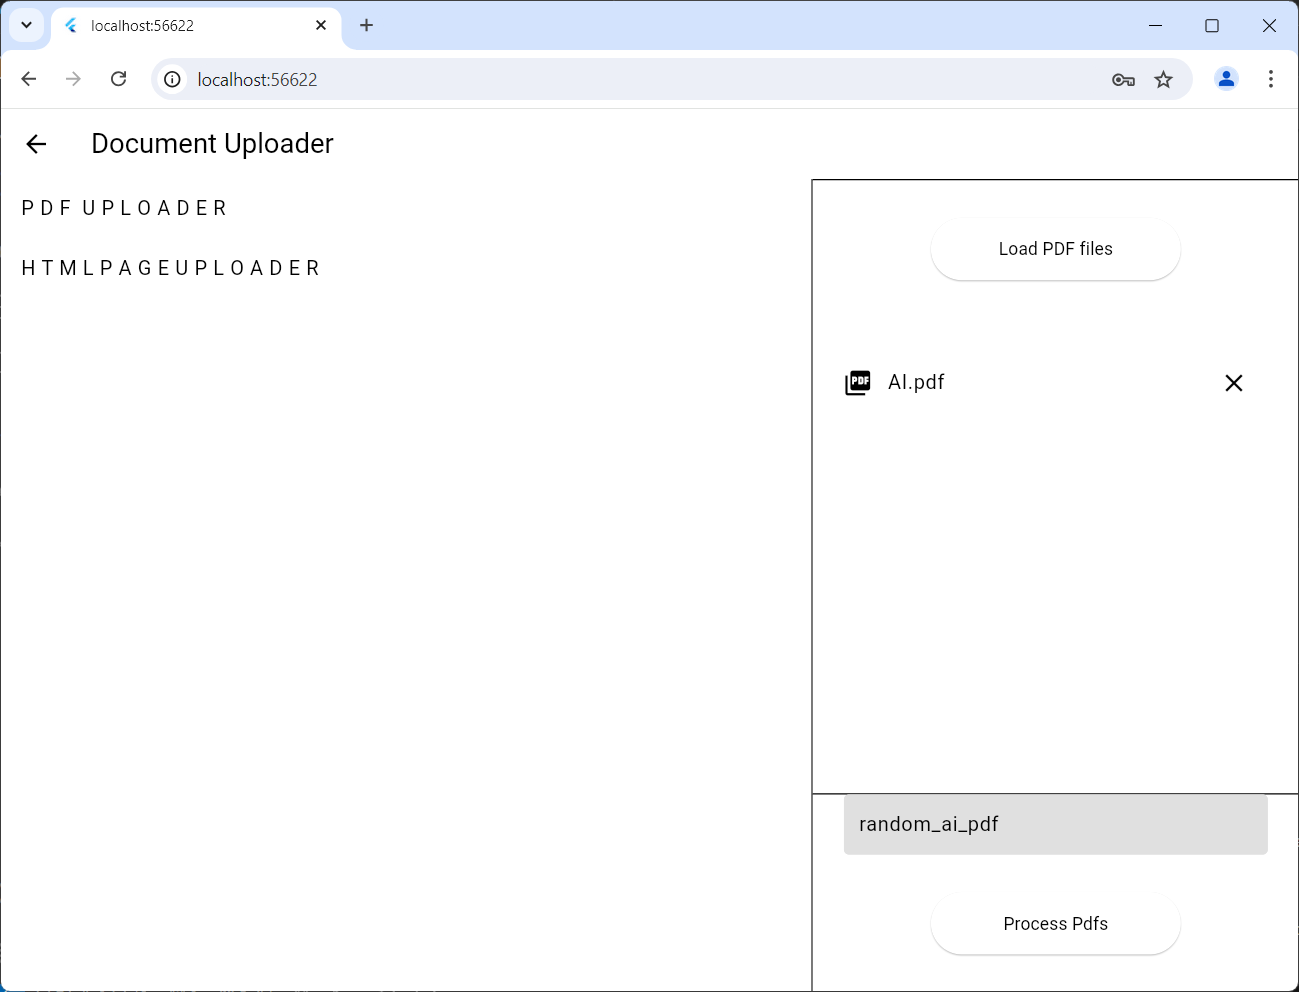
\includegraphics[width=0.45\linewidth]{Immagini/pdf_upload.png}
		\caption{Creazione di un nuovo contesto\newline}
		\label{fig:context-making}
	\end{subfigure}
	\begin{subfigure}{.5\textwidth}
		\centering
		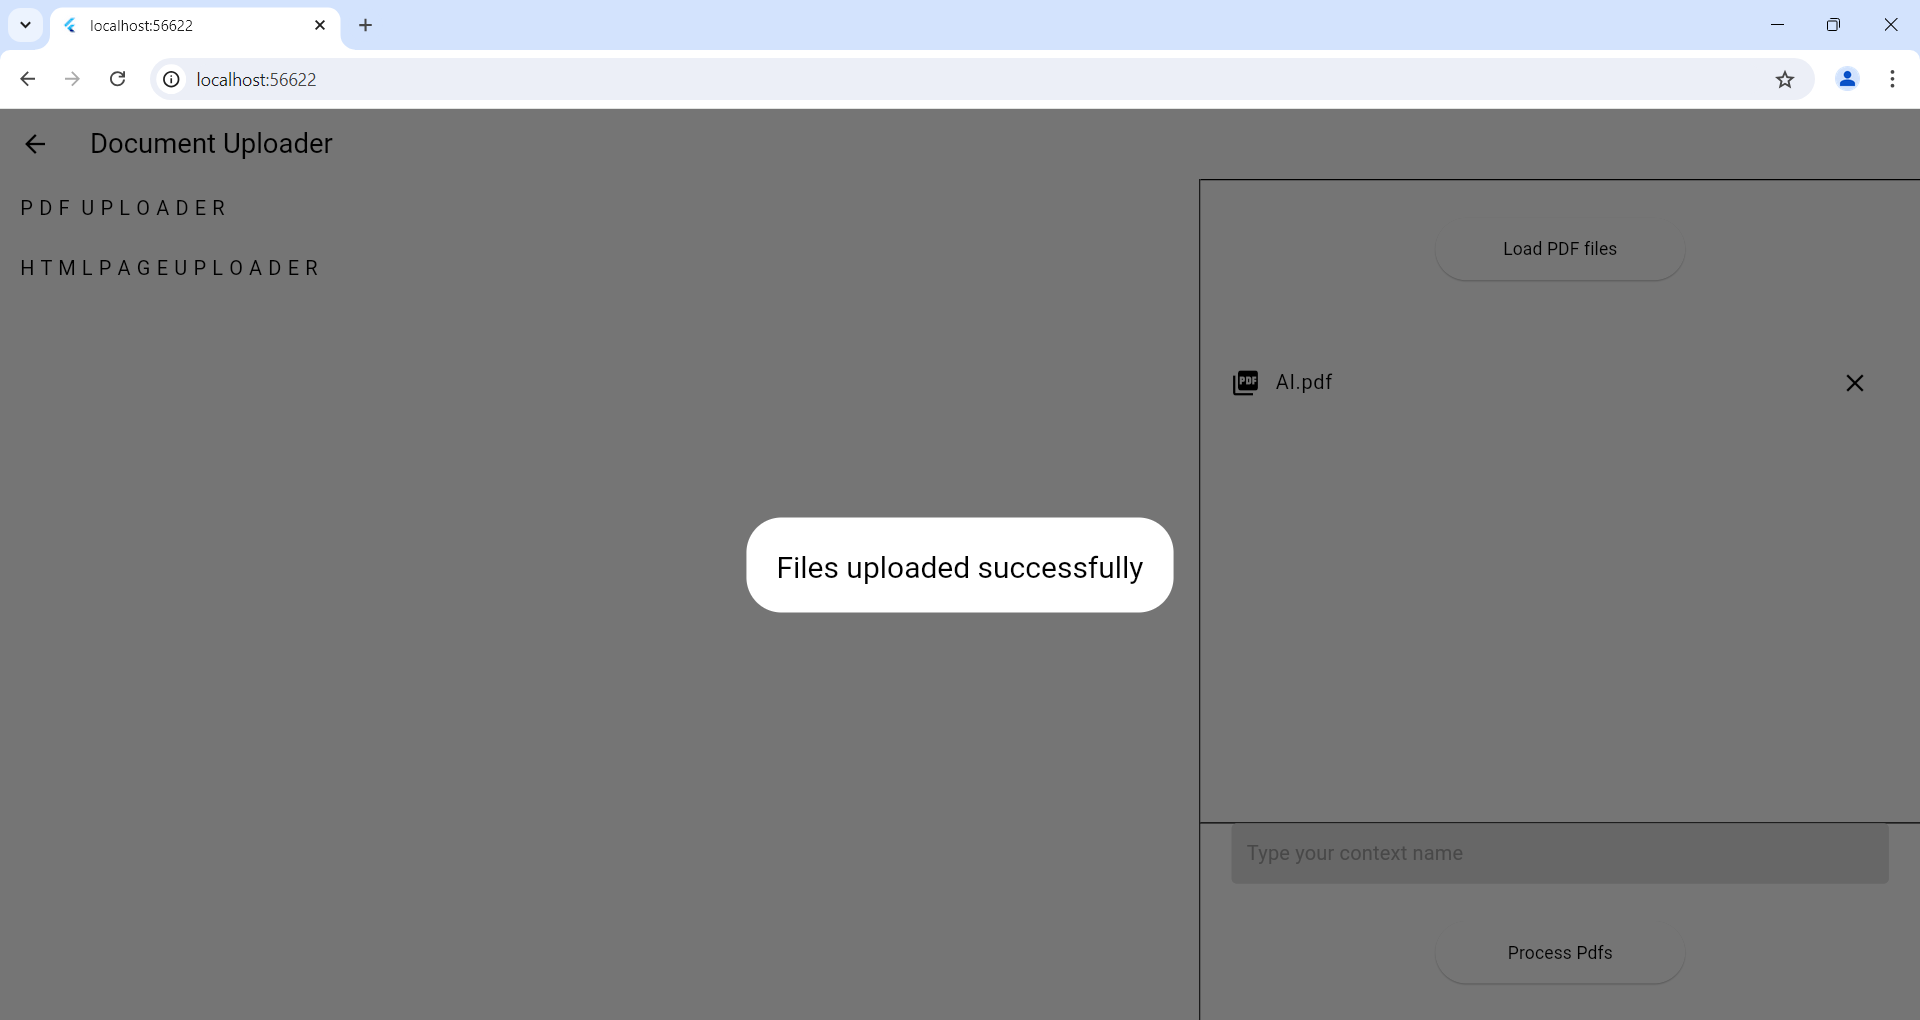
\includegraphics[width=0.45\linewidth]{Immagini/pdfs_successfully_upload.png}
		\caption{Notifica della creazione del nuovo contesto \newline}
		\label{fig:pdf_success}
	\end{subfigure}%
	\caption{Sezione per creare un nuovo contesto basato su documenti PDF}
\end{figure}

L'applicazione consente di creare un nuovo contesto utilizzando un insieme di file PDF, come illustrato nella figura \ref{fig:pdfs_context}, Inoltre, nella figura \ref{fig:pdf_removed}, è possibile osservare la funzionalità di rimozione di un documento tramite il pulsante "X" accanto al file. Questo pulsante elimina l'ultimo documento, rispetto a quanto mostrato nella figura \ref{fig:pdfs_context}.
\begin{figure}[H]
	\centering
        \begin{subfigure}{.5\textwidth}
		\centering
		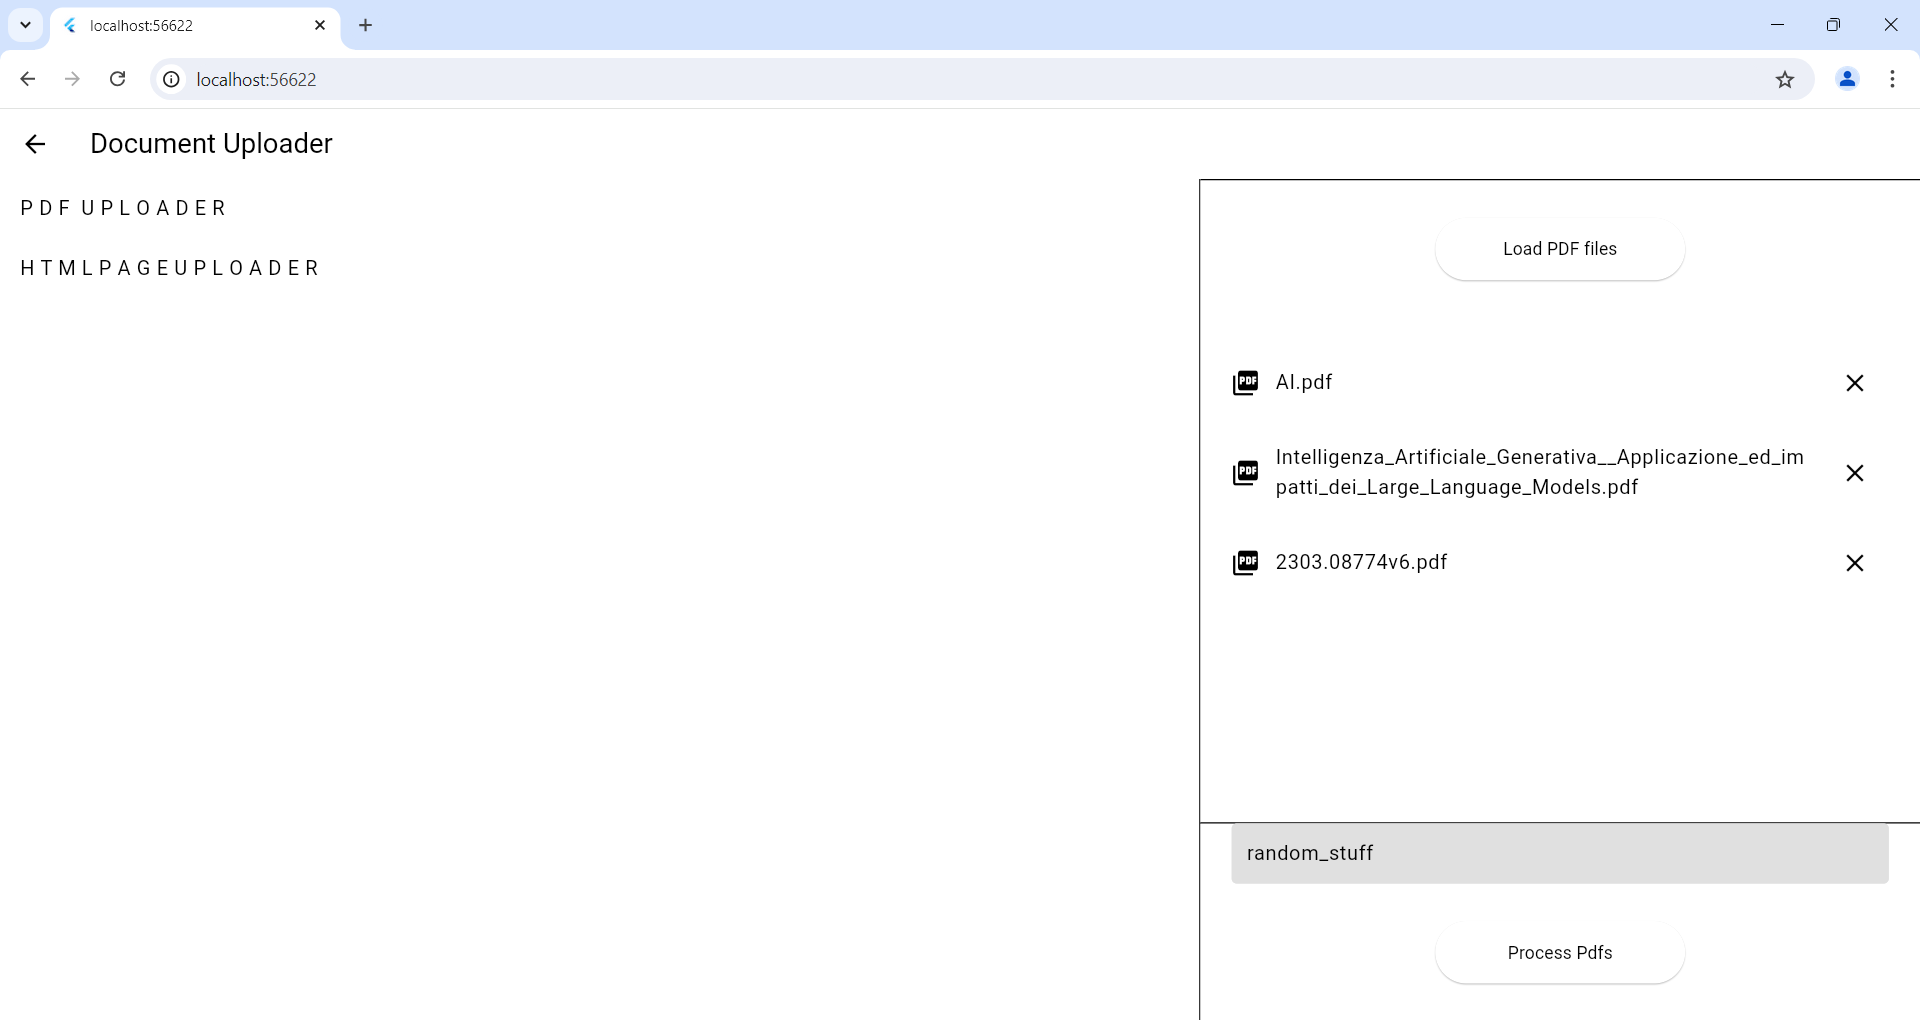
\includegraphics[width=0.45\linewidth]{Immagini/random_stuff.png}
		\caption{Creazione contesto con un'insieme di PDF\newline}
		\label{fig:pdfs_context}
	\end{subfigure}%
        \begin{subfigure}{.5\textwidth}
		\centering
		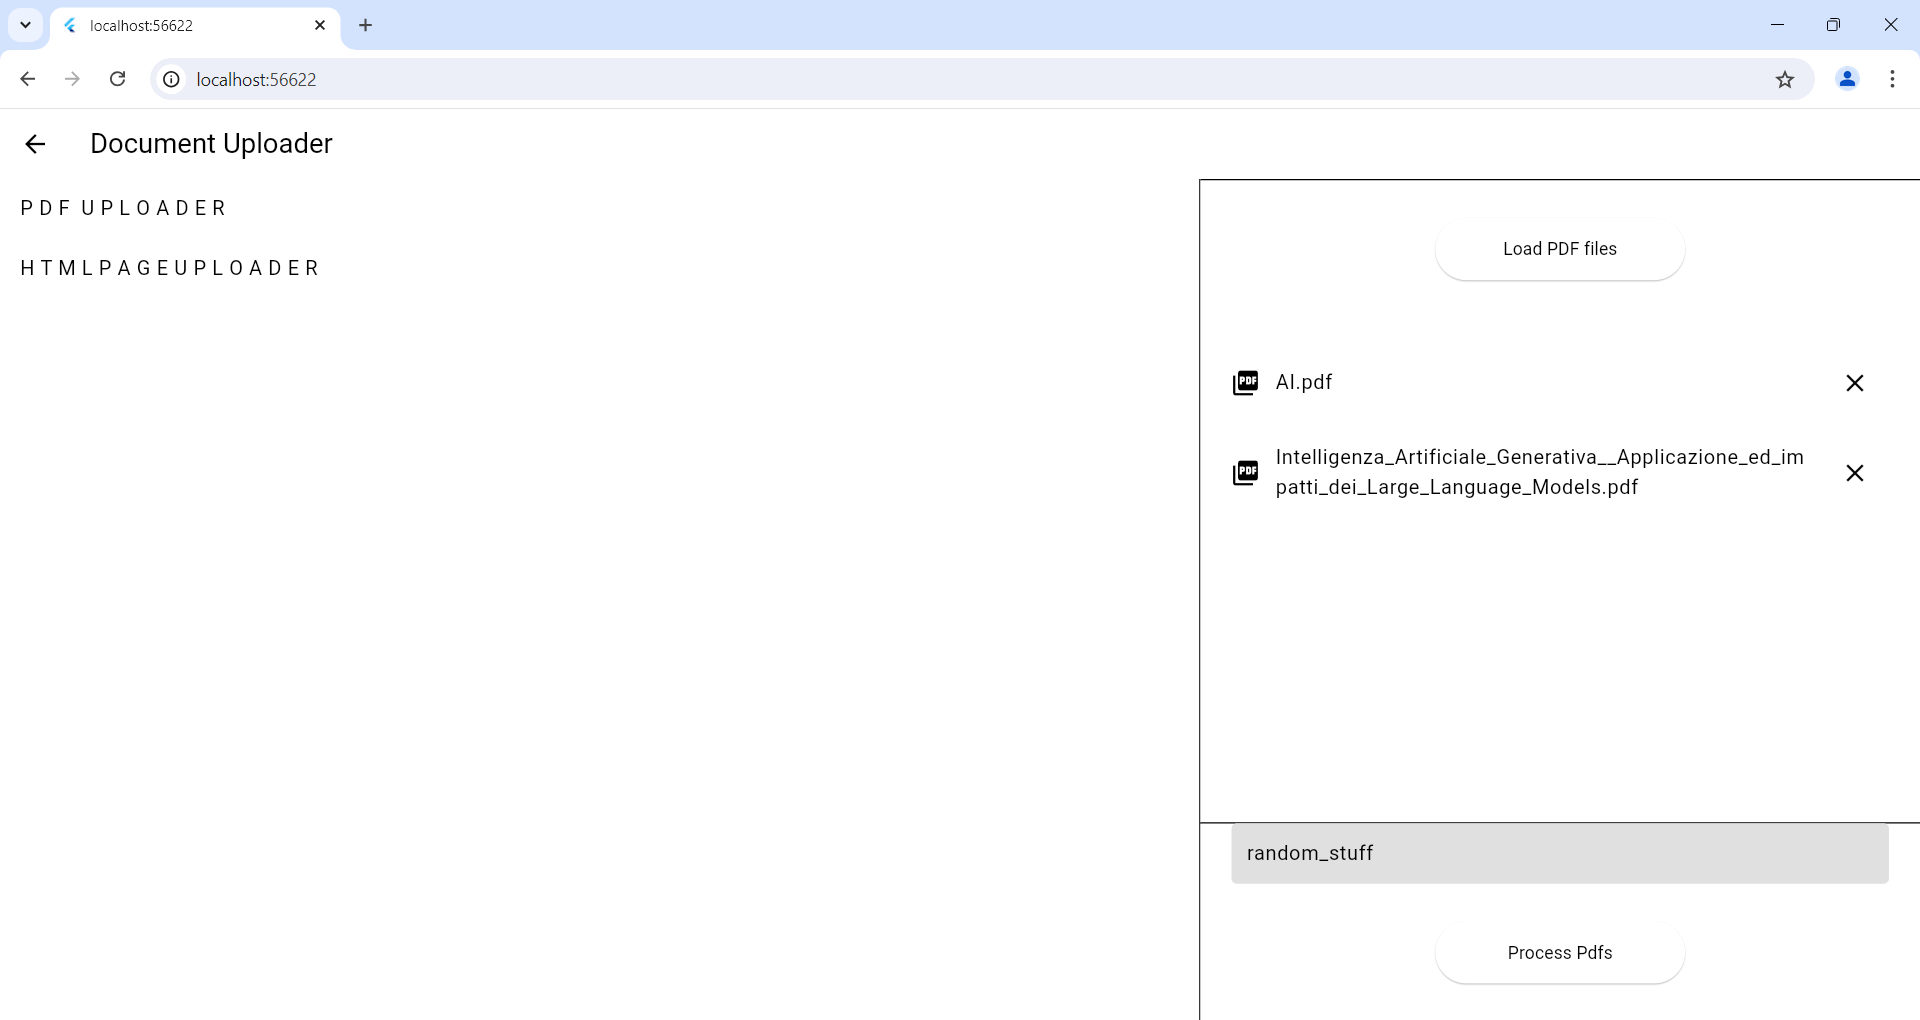
\includegraphics[width=0.45\linewidth]{Immagini/remove_one.png}
		\caption{Rimozione di un documento all'interno della lista\newline}
		\label{fig:pdf_removed}
	\end{subfigure}%
	\caption{Operazioni disponibili con la pagina di PDF Uploader}
\end{figure}

L'interfaccia per la creazione del contesto tramite pagine HTML è illustrata nella figura \ref{fig:html_section}. Essa include un campo per inserire gli URL delle pagine web, separati da un'interruzione di riga, e un pulsante per specificare il nome del contesto, come mostrato nella Figura \ref{fig:html_upload}.
Il processo per la creazione del contesto tramite pagine HTML è simile a quello per l'elaborazione dei PDF, con una sola differenza: una volta ricevuti gli URL, l'applicazione server estrae non solo le pagine HTML dai link forniti, ma anche le pagine figlie collegate all'interno di questi documenti, escludendo quelle che non appartengono al dominio specificato.

\begin{figure}[H]
	\centering
        \begin{subfigure}{.5\textwidth}
		\centering
		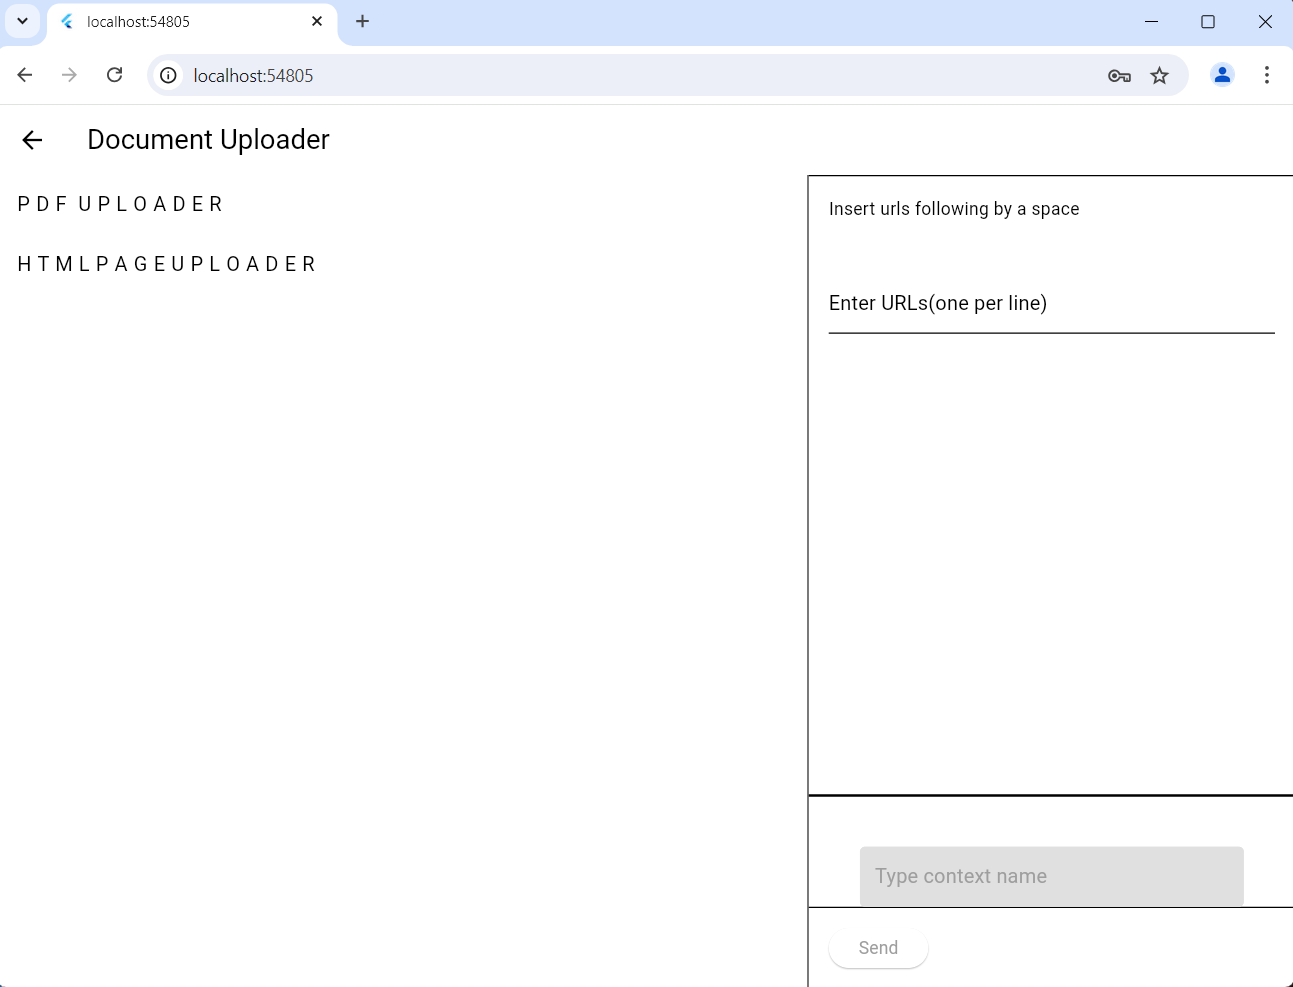
\includegraphics[width=0.45\linewidth]{Immagini/html_uploader_page.png}
		\caption{Sezione vuota per il caricamento di pagine HTML\newline}
		\label{fig:html_section}
	\end{subfigure}%
        \begin{subfigure}{.5\textwidth}
		\centering
		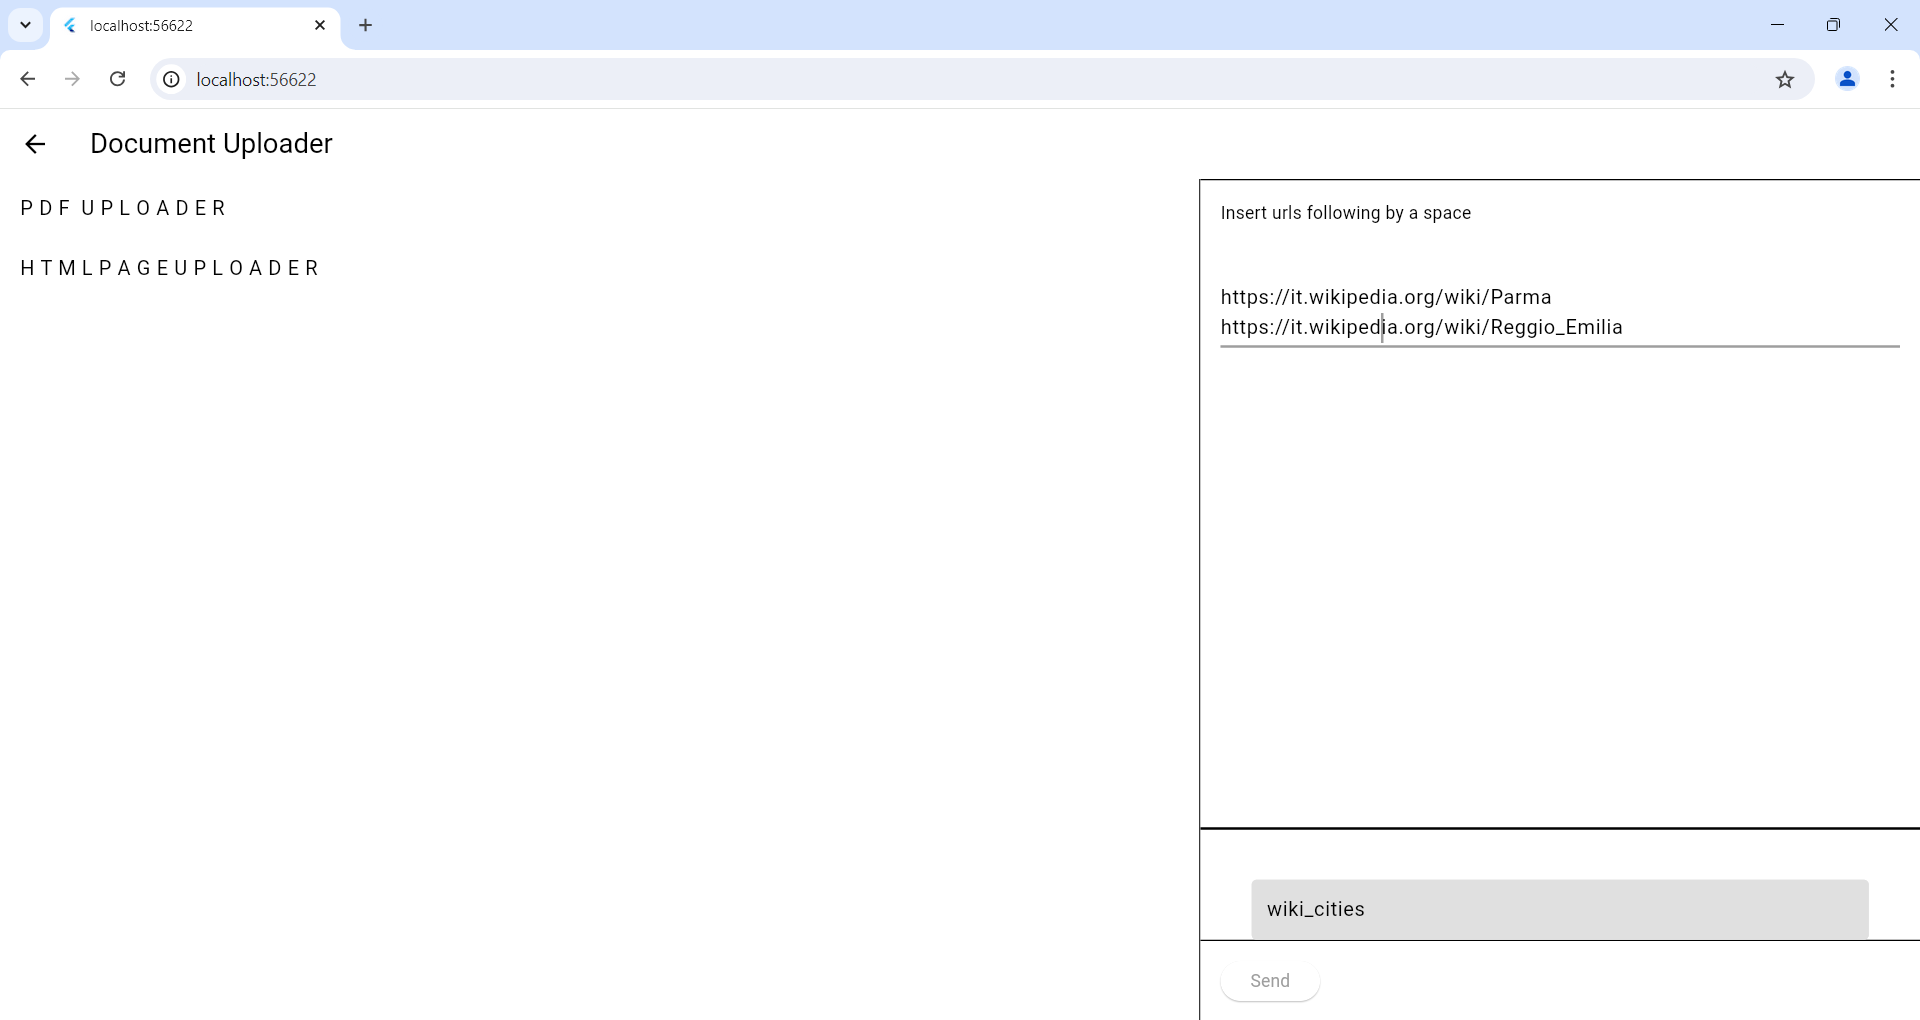
\includegraphics[width=0.45\linewidth]{Immagini/html_uploads.png}
		\caption{Rimozione di un documento all'interno della lista\newline}
		\label{fig:html_upload}
	\end{subfigure}%
	\caption{Sezione per il caricamento di Documenti HTML}
\end{figure}

\subsubsection{ChatBot}
La pagina del ChatBot consente all'utente di avviare una conversazione con un modello di linguaggio selezionando un contesto dalla sezione situata a destra, come mostrato nella Figura \ref{fig:chatbot}. Se la sezione è vuota, l'utente deve prima creare un contesto.

\begin{figure}[ht]
	\centering
	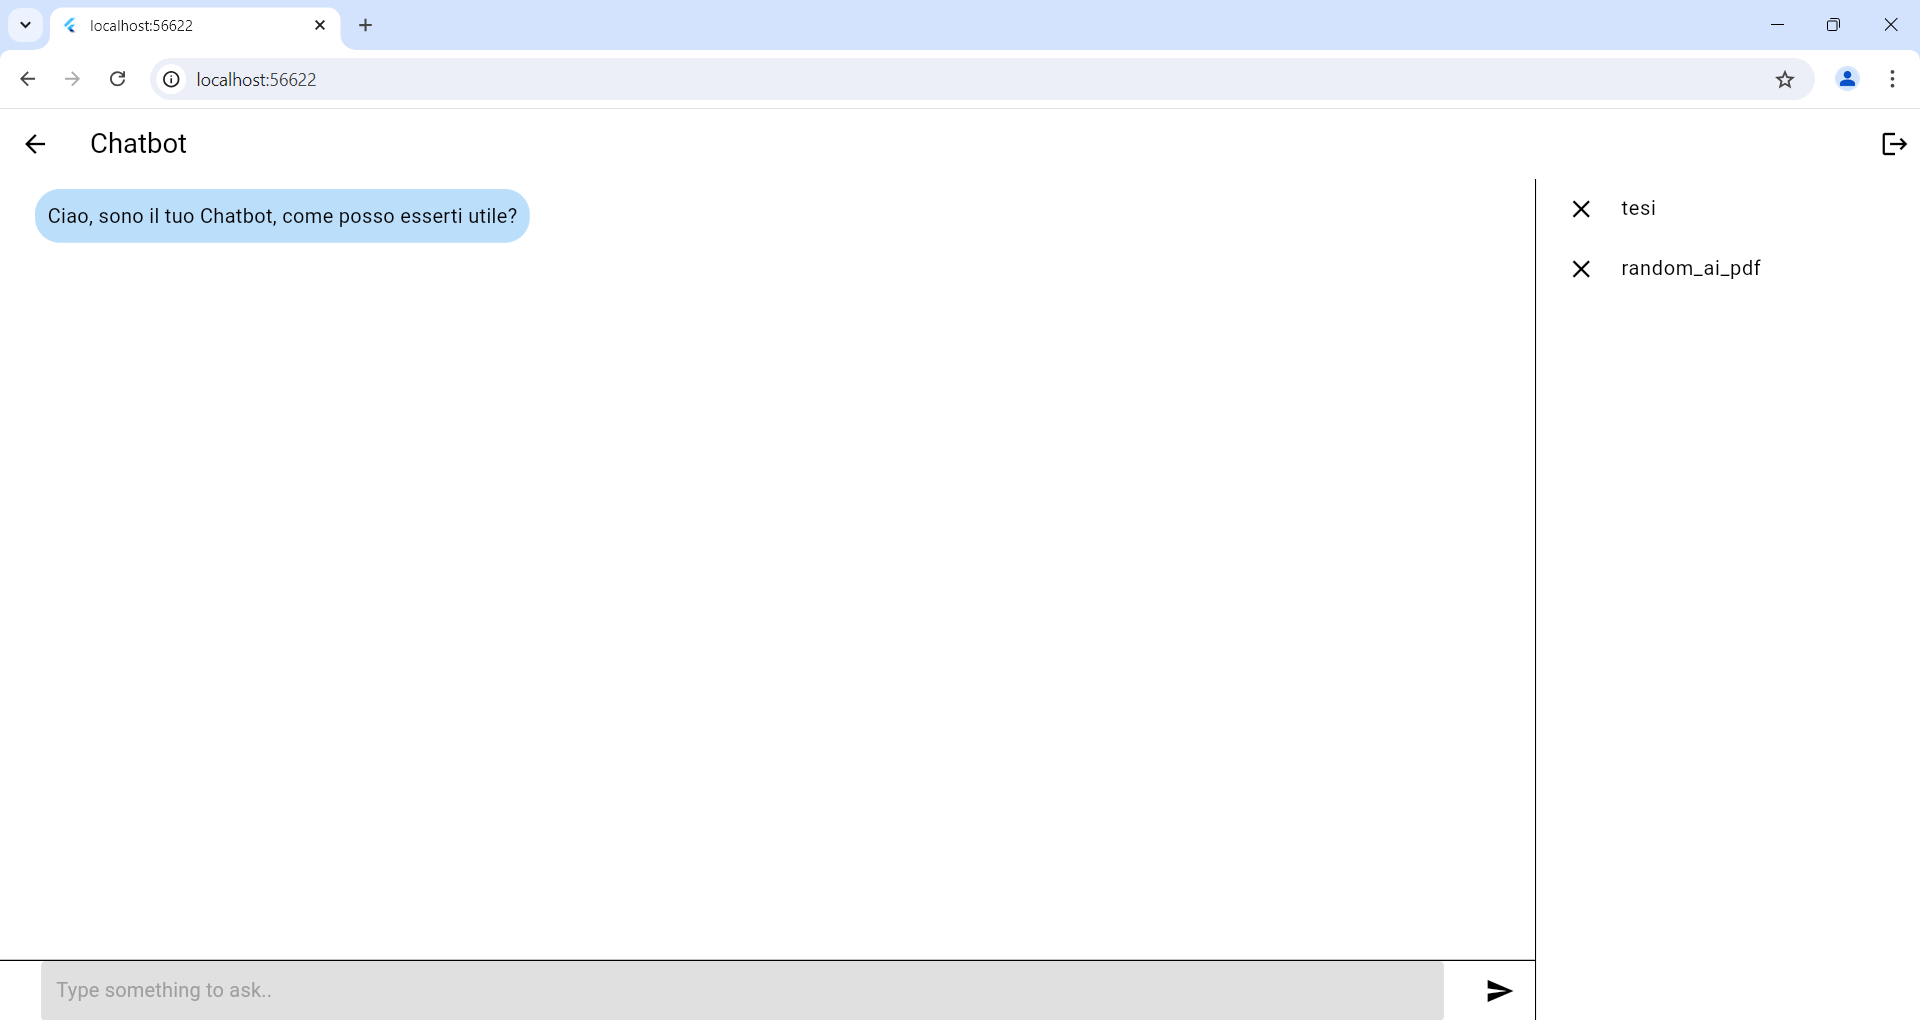
\includegraphics[width=0.3\textwidth]{Immagini/chatbot_page.png}
	\caption{Pagina del ChatBot dell'applicazione}
	\label{fig:chatbot}
\end{figure}
Una volta selezionato il contesto e inviata la domanda dall'utente, l'applicazione invia una richiesta HTTP al server, includendo la domanda e il contesto selezionato. Il server, tramite l'uso del retriever, recupera le informazioni pertinenti dal vettore di contesto presente nel database dell'utente e le integra nel prompt del modello di linguaggio. Successivamente, una volta generata la risposta, il server la invia all'applicazione. L'applicazione estrae quindi le informazioni dalla risposta HTTP e le visualizza a schermo tramite un messaggio per l'utente.
La Figura \ref{fig:chat} mostra alcune risposte generate dal modello di linguaggio e illustra il processo di comunicazione con il server.

\begin{figure}[H]
	\centering
        \begin{subfigure}{.5\textwidth}
		\centering
		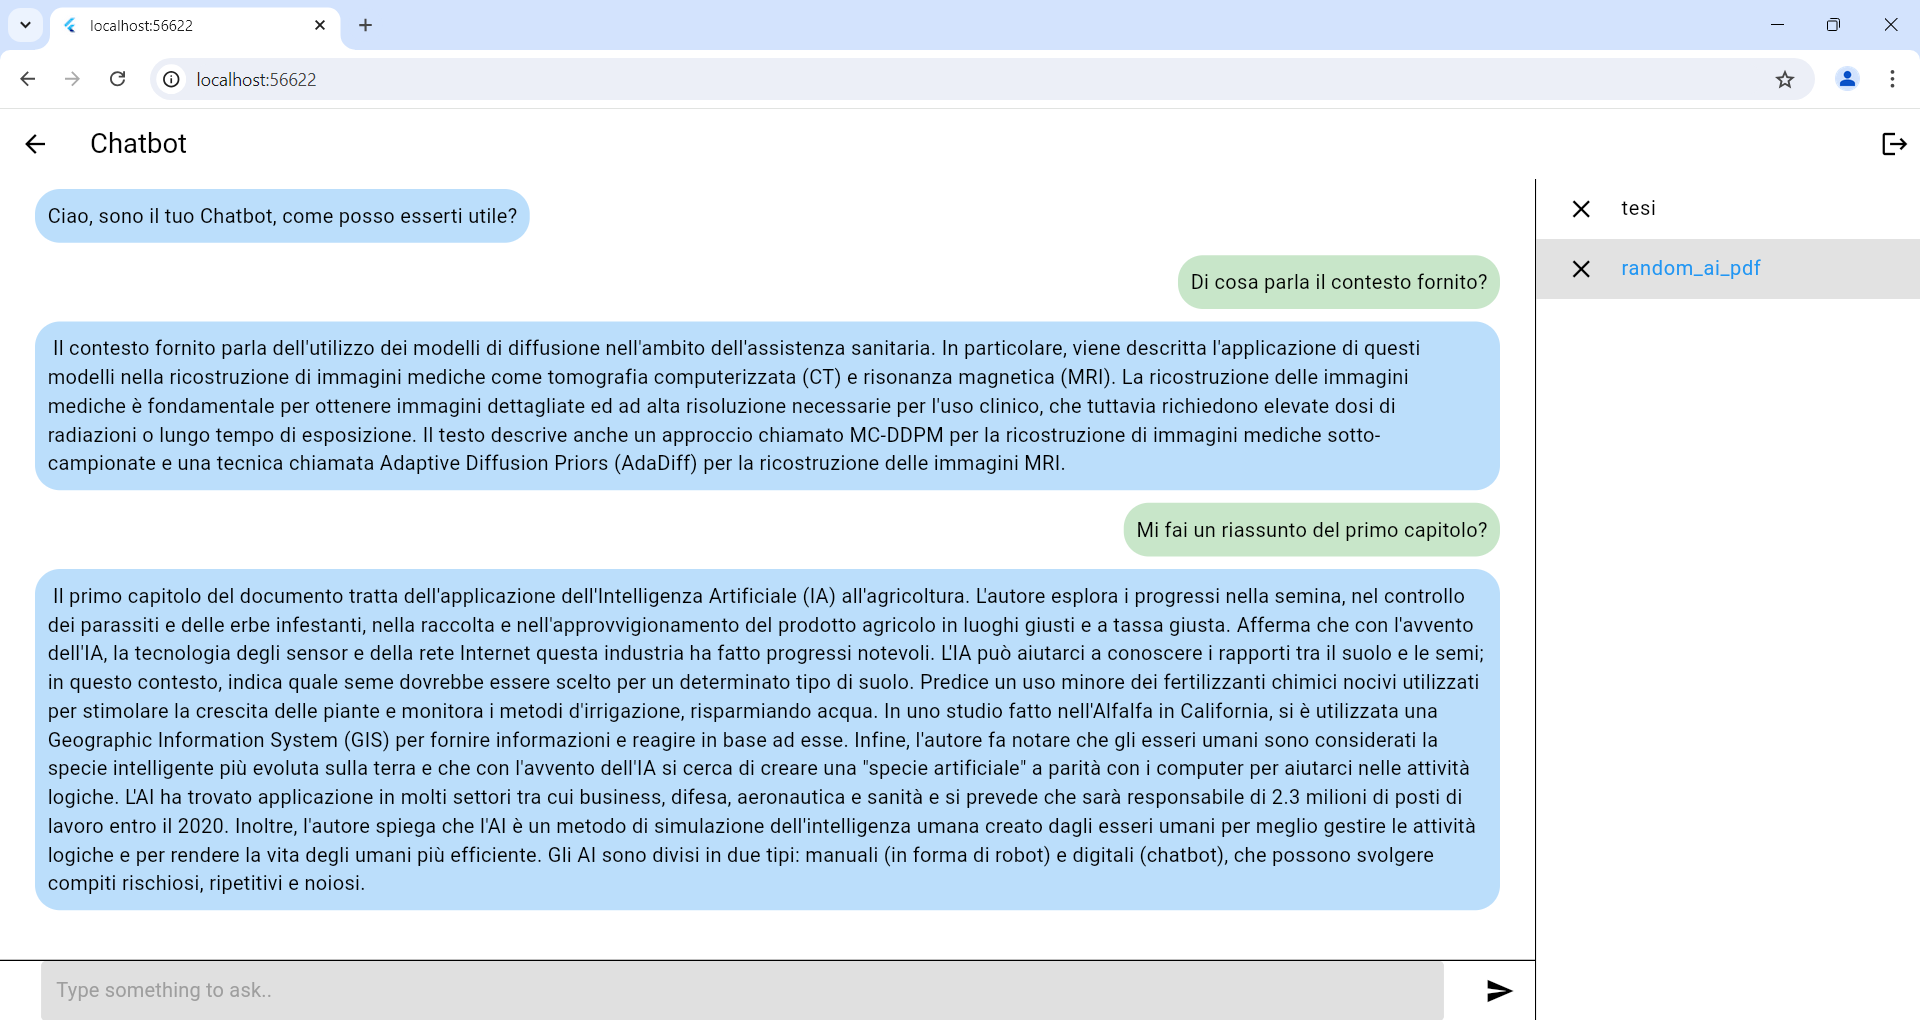
\includegraphics[width=0.45\linewidth]{Immagini/chat_example.png}
		\caption{Risposte generate dal modello linguaggio\newline}
	\end{subfigure}%
        \begin{subfigure}{.5\textwidth}
		\centering
		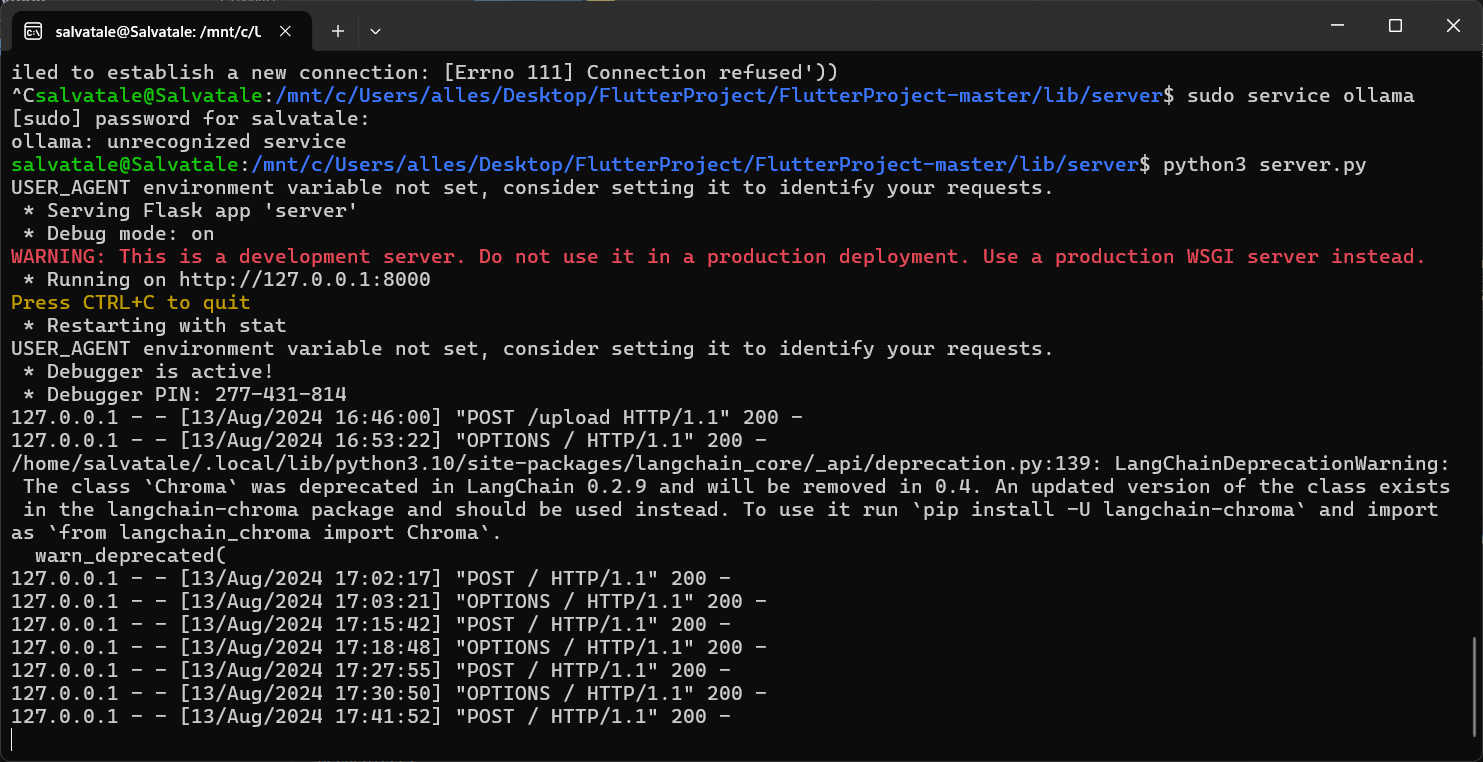
\includegraphics[width=0.45\linewidth]{Immagini/http_connections_during_conversation.png}
		\caption{Richieste HTTP generate dalla comunicazione tra server ed applicazione Flutter\newline}
	\end{subfigure}%
	\caption{Conversazione con il Chatbot}
        \label{fig:chat}
\end{figure}

\subsubsection{SpeechBot}
Lo speechbot permette all'utente di avere una conversazione vocale con il Bot come mostrato nella figura \ref{fig:speechbot}.
Il processo è simile a quello del ChatBot, ma con alcune differenze significative. Nel caso dello SpeechBot, l'utente deve registrare il proprio messaggio tramite microfono. L'applicazione converte l'audio in testo utilizzando la tecnologia Speech-to-Text. Successivamente, il messaggio ricevuto dal server viene convertito in audio tramite la tecnologia Text-to-Speech.
\begin{figure}[ht]
	\centering
	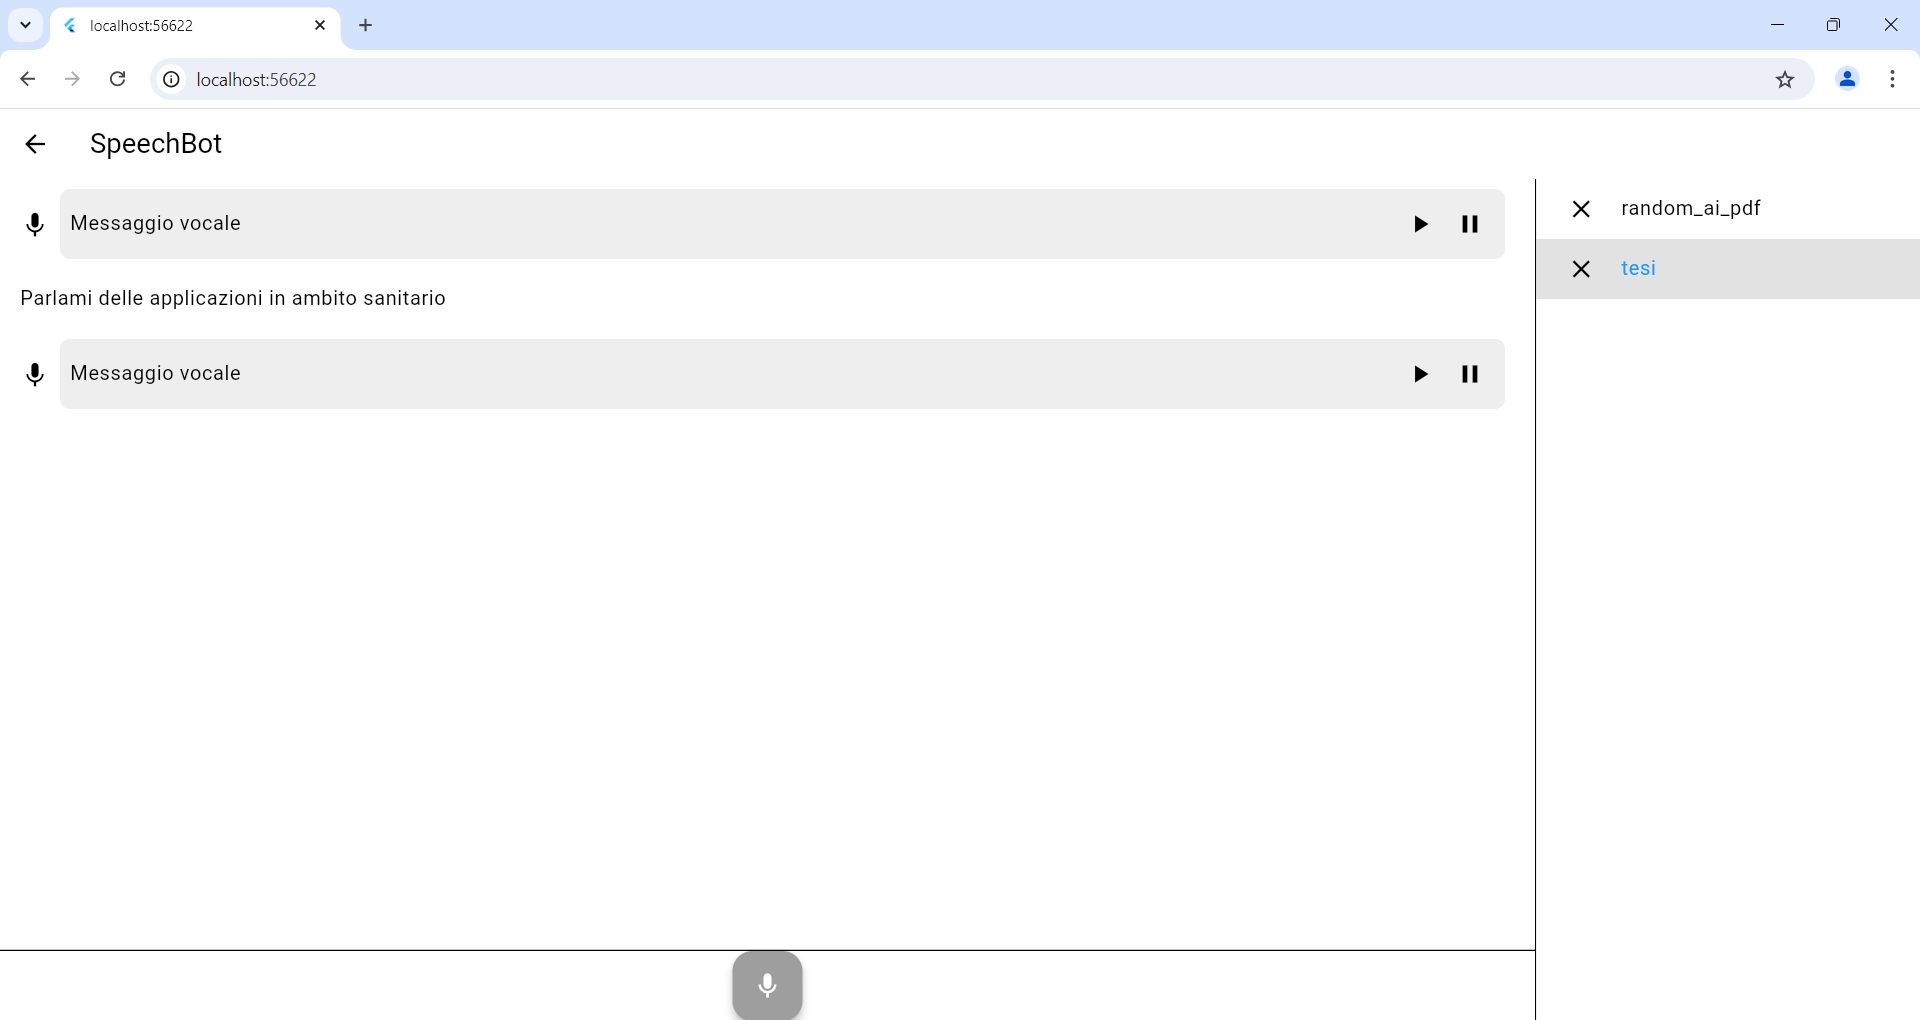
\includegraphics[width=0.3\textwidth]{Immagini/speechbot.png}
	\caption{Pagina dello SpeechBot dell'applicazione}
	\label{fig:speechbot}
\end{figure}

\section{Strumenti e tecnologie usate}

\subsection{Ollama}
Ollama è una piattaforma di supporto che funge da contenitore per modelli di linguaggio, analogamente a Docker per la gestione e distribuzione delle applicazioni. In particolare, Ollama consente di eseguire e gestire modelli di linguaggio all'interno di ambienti isolati e controllati, facilitando così la loro integrazione e distribuzione. La piattaforma offre anche la possibilità di scaricare i modelli in locale e di utilizzarli tramite codice Python.
Nell'ambito dell'applicazione, viene impiegato Mistral come modello di linguaggio di grandi dimensioni e nomic-embed-text come modello per l'embedding.

\subsection{Chroma}
Chroma è un database open-source ottimizzato per l'intelligenza artificiale, progettato per gestire e indicizzare grandi quantità di dati che le applicazioni AI utilizzano o generano. È costruito per essere altamente performante, scalabile e facile da integrare con altre applicazioni di machine learning o AI.
Nell'applicazione, Chroma fornisce i seguenti servizi: un database per l'archiviazione dei vettori relativi al contesto degli utenti, oltre a svolgere le funzioni di retriever e di generazione del vettore del contesto.

\subsection{Langchain}
LangChain è un framework progettato per facilitare la creazione di applicazioni basate su modelli di linguaggio, come GPT-4, attraverso la costruzione di catene di componenti interoperabili. Utilizzando il pacchetto LangChain in Python, è possibile sviluppare applicazioni avanzate basate su modelli di linguaggio sfruttando un'ampia gamma di funzionalità e componenti.
Nell'applicazione, LangChain fornisce l'integrazione di Ollama, Chroma e la gestione del prompt, consentendo di combinare questi elementi in un'architettura RAG. Questo permette al sistema di rispondere alle domande in modo contestuale, attingendo sia ai modelli di linguaggio che ai dati specifici degli utenti.

\subsection{Text-to-Speech}
Il pacchetto Flutter utilizzato per convertire il testo in audio all'interno dell'applicazione è 'flutter\_tts'. Questo pacchetto offre funzionalità di sintesi vocale, permettendo all'applicazione di trasformare il testo in audio in modo fluido e integrato.

\subsection{Speech-To-Text}
Il pacchetto Flutter utilizzato per convertire l'audio in testo all'interno dell'applicazione è speech\_to\_text. Questo pacchetto fornisce funzionalità di riconoscimento vocale, permettendo all'applicazione di trascrivere l'audio in testo in modo efficace e preciso.

\subsection{Flask}
Flask è un framework web leggero per Python, progettato per facilitare la creazione di applicazioni web in modo rapido e semplice, mantenendo al contempo la flessibilità necessaria per gestire applicazioni complesse.
All'interno dell'applicazione viene utilizzato per ricevere ed inviare richieste HTTP tra Flutter ed il server.

\section{Prestazioni Chatbot ed obiettivi futuri}

\subsection{Performance}
Il Chatbot, in termini di prestazioni, risulta mediocre. Sebbene le risposte siano per lo più corrette, sono spesso molto sintetiche e talvolta il sistema fatica a comprendere le domande. Inoltre, i tempi di generazione sono piuttosto lunghi, variando in base all'architettura su cui è in esecuzione. 
Quando il Chatbot opera su una GPU di basso livello, la generazione delle risposte richiede circa 1-2 minuti. Questo suggerisce che, se gestito con una GPU di buona qualità, la generazione delle risposte potrebbe avvenire in modo quasi istantaneo, migliorando notevolmente le prestazioni complessive del sistema.
Considerando i tempi di attesa significativamente lunghi quando si utilizza solo la CPU, è stata aggiunta la possibilità di implementare il MailBot. Questo permette di inviare le risposte via email, in modo che l'utente non debba attendere il completamento della generazione direttamente nell'interfaccia, migliorando l'esperienza complessiva.
Per quanto riguarda la creazione del vettore del contesto, anche con l'uso di GPU, questo processo può risultare estremamente lungo. Sebbene non rappresenti un problema sostanziale per l'utente, poiché il processo può essere gestito in background, costituisce un limite significativo per le risorse computazionali. Infatti, il lungo tempo di elaborazione potrebbe rallentare altri processi in esecuzione, influenzando negativamente le prestazioni complessive del sistema.

\subsection{Obiettivi futuri e possinili applicazioni}
Per migliorare il Chatbot e ampliare le sue capacità, si potrebbero considerare diverse nuove funzionalità. Una delle principali aggiunte sarebbe la possibilità per l'utente di scegliere la lingua di generazione delle risposte o di selezionare il modello di linguaggio preferito tra quelli disponibili. Questo permetterebbe una personalizzazione maggiore e una maggiore flessibilità nell'interazione con il sistema.
Un'altra modifica che l'utente può compiere potrebbe essere la capacità di abbassare il parametro "temperature" che permette al modello di aumentare la serietà delle risposte tanto più alto il valore, questo darebbe la capacità al modello di generare risposte fantasiose quando parla con un bambino.
Inoltre, sarebbe utile offrire agli utenti la possibilità di gestire i propri contesti con maggiore facilità. Attualmente, l'applicazione consente di creare un contesto tramite la pagina del "Doc Uploader" e di eliminarlo tramite un semplice clic sulla "X" accanto al contesto nella sezione a destra delle pagine di Chat. Questa funzionalità potrebbe essere ulteriormente affinata per una gestione più intuitiva e completa dei contesti.
Un'altra possibile implementazione è un'interfaccia nella pagina di "SpeechBot" che simuli una chiamata vocale, offrendo un'interazione più naturale e immediata tra l'utente e il Chatbot. Questa funzionalità potrebbe migliorare l'esperienza utente, rendendo la comunicazione più fluida e coinvolgente.
\newline

Il chatbot potrebbe essere utilizzato per l'elaborazione di documenti e per la specializzazione in determinati contesti, rivelandosi un supporto prezioso per le persone in diversi ambiti. Ad esempio, potrebbe essere impiegato in un museo per rispondere a domande dei turisti riguardanti la storia delle opere e delle sculture, offrendo informazioni dettagliate e contestualizzate. In ambito educativo, potrebbe assistere gli studenti nella preparazione di esami, permettendo loro di salvare contesti specifici come "esame", formulare domande ed esercizi, e verificare le risposte ottenute. Inoltre, il chatbot potrebbe rappresentare un aiuto significativo per i professori, facilitando la generazione di domande casuali per esami o esercitazioni e migliorando l'efficienza nella preparazione e gestione delle prove. Implementando tali funzionalità, il chatbot diventa uno strumento estremamente versatile e utile in una varietà di contesti.
Gli usi finora elencati sono solo alcune delle possibili applicazioni del chatbot. A seconda delle esigenze specifiche dell'utente, il chatbot può essere adattato e personalizzato per soddisfare una vasta gamma di scenari e requisiti. La sua versatilità consente di ottimizzare le sue funzionalità per rispondere a necessità diverse e variabili.

%
%
%%%% Le Conclusioni
\pagestyle{plain}
\chapter*{Conclusione} %Se si cambia il Titolo cambiare anche la riga successiva così che appia corretto nell'conclusione
\addcontentsline{toc}{chapter}{Conclusione} %Per far apparire Introduzione nell'indice (Il nome deve rispecchiare quello del chapter)
In conclusione, i modelli di grandi dimensioni si confermano come strumenti di grande valore in numerosi ambiti professionali, tra cui il business, la medicina e la cybersecurity. Tuttavia, il loro impiego solleva preoccupazioni significative riguardo alla privacy, alla sicurezza, alla diffusione di disinformazione e ai bias. È essenziale che, nel prossimo futuro, vengano adottati regolamenti più rigorosi e sviluppate tecniche avanzate per proteggere i dati e garantire la privacy delle informazioni. Pur riconoscendo i benefici notevoli delle intelligenze artificiali generative, è fondamentale essere consapevoli dei rischi concreti associati al loro uso e affrontarli con la dovuta attenzione e responsabilità.
In aggiunta, questo studio ha delineato un nuovo approccio allo sviluppo, dimostrando come i modelli di grandi dimensioni (LLMs) possano essere applicati a casi d'uso pratici. Un esempio concreto di applicazione open-source è stato presentato, mettendo in luce come l’accessibilità di questi strumenti consenta a chiunque di implementare soluzioni innovative. Tuttavia, questa stessa accessibilità comporta il rischio di utilizzi non leciti. Pertanto, è cruciale non solo valorizzare le potenzialità di queste tecnologie, ma anche affrontare i potenziali abusi e adottare misure adeguate per mitigare tali rischi, bilanciando l'innovazione tecnologica con la necessità di proteggere gli aspetti etici e sociali della nostra vita digitale.

%
%%%% La bibliografia
\bibliographystyle{apalike} %{plain} -- Scegliere lo stile preferito
\cleardoublepage
\addcontentsline{toc}{chapter}{\bibname}
\bibliography{./Bibliografia}
%
%\include{Capitoli/Ringraziamenti}
%
% Le appendici
\appendix
\chapter{Appendice: Codice sorgente}
In questa appendice e' riportato il codice sorgente utilizzato nel progetto.
\section{Codice in Python del server}
\begin{lstlisting}[style=pythonstyle,caption={Codice del server.py}, label={lst:server}]
from flask import Flask, json, request, jsonify
from chatbot import process_input
from mail_chatbot import send_email
import vector_db_maker as vector
import directory_manager as dm
app = Flask(__name__)
@app.route('/upload', methods=['OPTIONS', 'POST'])
async def upload_file():
    if request.method == 'OPTIONS':
        # Gestisci la richiesta OPTIONS
        response = app.make_default_options_response()
        # Aggiungi i metodi consentiti nella risposta
        response.headers['Access-Control-Allow-Methods'] = 'POST'
        # Aggiungi gli header consentiti nella risposta
        response.headers['Access-Control-Allow-Headers'] = 'Content-Type'
    elif request.method == 'POST':
        directory_name = "./data/"
        if 'jsonFile' in request.files :
            json_data = request.files['jsonFile'].read()
            json_dict = json.loads(json_data)
            directory_name += json_dict['userID'] + '/' + json_dict['directory_name']
        if 'files' not in request.files:
            return jsonify({'error': 'No file part'}), 400
        uploaded_files = request.files.getlist("files")
        file_names = []
        for file in uploaded_files:
            file.save(file.filename)
            file_names.append(file.filename)
        await vector.get_text(uploaded_files, directory_name)
        response = jsonify({'message': 'Files uploaded successfully', 'files': file_names})
    # Aggiungi gli header CORS alla risposta per consentire le richieste da origini diverse
    response.headers['Access-Control-Allow-Origin'] = '*'  # Cambia '*' con l'origine desiderata
    response.headers['Access-Control-Allow-Headers'] = 'Content-Type'
    return response
@app.route('/create_directory', methods=['OPTIONS', 'POST'])
def handle_create_directory():
    if request.method == 'OPTIONS':
        # Gestisci la richiesta OPTIONS
        response = app.make_default_options_response()
        # Aggiungi i metodi consentiti nella risposta
        response.headers['Access-Control-Allow-Methods'] = 'POST'
        # Aggiungi gli header consentiti nella risposta
        response.headers['Access-Control-Allow-Headers'] = 'Content-Type'
    elif request.method == 'POST':
        # Gestisci la richiesta POST
        data = request.json  # Ottieni i dati JSON dalla richiesta
        # Fai qualcosa con i dati ricevuti, ad esempio, restituisci una risposta
        user_id = data['userId']
        dm.create_user_directory(user_id)
        response = jsonify({'message': "user directory created"})
    else:
        # Se il metodo non e' OPTIONS o POST, restituisci un errore
        response = jsonify({'error': 'Metodo non supportato'})
        response.status_code = 405  # Metodo non consentito
    # Aggiungi gli header CORS alla risposta per consentire le richieste da origini diverse
    response.headers['Access-Control-Allow-Origin'] = '*'  # Cambia '*' con l'origine desiderata
    response.headers['Access-Control-Allow-Headers'] = 'Content-Type'
    return response
@app.route('/directory', methods=['OPTIONS', 'POST'])
def handle_request_directory():
    if request.method == 'OPTIONS':
        # Gestisci la richiesta OPTIONS
        response = app.make_default_options_response()
        # Aggiungi i metodi consentiti nella risposta
        response.headers['Access-Control-Allow-Methods'] = 'POST'
        # Aggiungi gli header consentiti nella risposta
        response.headers['Access-Control-Allow-Headers'] = 'Content-Type'
    elif request.method == 'POST':
        # Gestisci la richiesta POST
        data = request.json  # Ottieni i dati JSON dalla richiesta
        # Fai qualcosa con i dati ricevuti, ad esempio, restituisci una risposta
        user_id = data['userId']
        directory_list = dm.get_user_directory(user_id)
        response = jsonify({'directory_list': directory_list})
    else:
        # Se il metodo non e' OPTIONS o POST, restituisci un errore
        response = jsonify({'error': 'Metodo non supportato'})
        response.status_code = 405  # Metodo non consentito
    # Aggiungi gli header CORS alla risposta per consentire le richieste da origini diverse
    response.headers['Access-Control-Allow-Origin'] = '*'  # Cambia '*' con l'origine desiderata
    response.headers['Access-Control-Allow-Headers'] = 'Content-Type'
    return response
@app.route('/', methods=['OPTIONS', 'POST'])
def handle_request():
    if request.method == 'OPTIONS':
        # Gestisci la richiesta OPTIONS
        response = app.make_default_options_response()
        # Aggiungi i metodi consentiti nella risposta
        response.headers['Access-Control-Allow-Methods'] = 'POST'
        # Aggiungi gli header consentiti nella risposta
        response.headers['Access-Control-Allow-Headers'] = 'Content-Type'
    elif request.method == 'POST':
        # Gestisci la richiesta POST
        data = request.json  # Ottieni i dati JSON dalla richiesta
        # Fai qualcosa con i dati ricevuti, ad esempio, restituisci una risposta
        path_directory = "./data/" + data['userId'] + "/" + data['context']
        response_data = process_input(data['message'],path_directory)
        if data['function'] == 'message':
            response = jsonify({'message': response_data})
        elif data['function'] == 'mail':
            send_email(response_data,data['mail'],data['message'])
            response = jsonify({'message': 'mail sent'})
    else:
        # Se il metodo non e' OPTIONS o POST, restituisci un errore
        response = jsonify({'error': 'Metodo non supportato'})
        response.status_code = 405  # Metodo non consentito
    # Aggiungi gli header CORS alla risposta per consentire le richieste da origini diverse
    response.headers['Access-Control-Allow-Origin'] = '*'  # Cambia '*' con l'origine desiderata
    response.headers['Access-Control-Allow-Headers'] = 'Content-Type'
    return response
@app.route('/url', methods=['OPTIONS', 'POST'])
async def handle_url_request():
    if request.method == 'OPTIONS':
        # Gestisci la richiesta OPTIONS
        response = app.make_default_options_response()
        # Aggiungi i metodi consentiti nella risposta
        response.headers['Access-Control-Allow-Methods'] = 'POST'
        # Aggiungi gli header consentiti nella risposta
        response.headers['Access-Control-Allow-Headers'] = 'Content-Type'
    elif request.method == 'POST':
        # Gestisci la richiesta POST
        data = request.json  # Ottieni i dati JSON dalla richiesta
        # Fai qualcosa con i dati ricevuti, ad esempio, restituisci una risposta
        path_directory = "./data/" + data['userId'] + "/" + data['context']
        urls = str(data["message"])
        print(urls)
        await vector.urls_vectordb_maker(urls,path_directory)
        response = jsonify({'message': "Vectordb created successfully"})
    else:
        # Se il metodo non e' OPTIONS o POST, restituisci un errore
        response = jsonify({'error': 'Metodo non supportato'})
        response.status_code = 405  # Metodo non consentito
    # Aggiungi gli header CORS alla risposta per consentire le richieste da origini diverse
    response.headers['Access-Control-Allow-Origin'] = '*'  # Cambia '*' con l'origine desiderata
    response.headers['Access-Control-Allow-Headers'] = 'Content-Type'
    return response
if __name__ == '__main__':
    app.run(debug=True,port=8000)
\end{lstlisting}
\begin{lstlisting}[style=pythonstyle,caption={Codice del chatbot.py}, label={lst:chatbot}]
from langchain_community.vectorstores import Chroma
from langchain_community import embeddings
from langchain_community.llms import Ollama
from langchain_core.runnables import RunnablePassthrough
from langchain_core.output_parsers import StrOutputParser
from langchain_core.prompts import ChatPromptTemplate
import os
def process_input(question,persist_directory):
    if not os.path.exists(persist_directory):
        return "Invalid context, insert a valid context!!"
    db = Chroma(persist_directory=persist_directory, embedding_function=embeddings.OllamaEmbeddings(model='nomic-embed-text'))
    retriever = db.as_retriever()
    model_local = Ollama(model="mistral")
    #perform the RAG 
    question = "rispondi in italiano a: " + question
    after_rag_template = """Answer the question based only on the following context:
    {context}
    Question: {question}
    """
    after_rag_prompt = ChatPromptTemplate.from_template(after_rag_template)
    after_rag_chain = (
        {"context": retriever, "question": RunnablePassthrough()}
        | after_rag_prompt
        | model_local
        | StrOutputParser()
    )
    return after_rag_chain.invoke(question)
\end{lstlisting}
\begin{lstlisting}[style=pythonstyle,caption={Codice del mail\_chatbot.py}, label={lst:mailchatbot}]
import smtplib
from email.mime.text import MIMEText
def send_email(response,receiver_mail,question):
        server = smtplib.SMTP("smtp.gmail.com", 587)
        server.starttls()
        server.login("alle.salva7@gmail.com","**************")
        text = "Question: " + question + "\n" + "Risposta: " + response
        msg = MIMEText(text, _charset='utf-8')
        msg['From'] = "alle.salva7@gmail.com"
        msg['To'] = receiver_mail
        msg['Subject'] = "CHATBOT response"
        server.sendmail(msg['From'],msg['To'],msg.as_string())
        server.quit()
\end{lstlisting}
\begin{lstlisting}[style=pythonstyle,caption={Codice del directory\_manager.py}, label={lst:directorymanager}]
import os
def get_user_directory(user_id):
    directory = "./data/" + user_id
    elements = os.listdir(directory)
    directory_list = [element for element in elements if os.path.isdir(os.path.join(directory,element))]
    return directory_list
def create_user_directory(user_id):
    path_directory = "./data/" + user_id
    os.mkdir(path_directory)
\end{lstlisting}
\begin{lstlisting}[style=pythonstyle,caption={Codice del url\_parser.py}, label={lst:urlparser}]
import requests
from bs4 import BeautifulSoup
from urllib.parse import urlparse, urljoin
def get_same_domain_links(url):
    # Ottieni il contenuto HTML della pagina
    response = requests.get(url)
    # Controlla che la richiesta sia andata a buon fine
    if response.status_code == 200:
        # Analizza il contenuto HTML
        soup = BeautifulSoup(response.content, 'html.parser')
        # Ottieni il dominio base dell'URL passato
        base_domain = urlparse(url).netloc
        # Trova tutti i tag 'a' che contengono i link
        links = soup.find_all('a', href=True)
        # Lista per salvare i link con la stessa radice dell'URL passato
        same_domain_links = []
        for link in links:
            # Ottieni l'URL completo del link
            href = link['href']
            # Unisci l'URL relativo con l'URL di base per ottenere l'URL completo
            full_url = urljoin(url, href)
            # Controlla se l'URL appartiene allo stesso dominio dell'URL passato
            if urlparse(full_url).netloc == base_domain:
                same_domain_links.append(full_url)
        return same_domain_links
    else:
        # Se la richiesta non e' andata a buon fine, restituisci una lista vuota
        return []
\end{lstlisting}
\begin{lstlisting}[style=pythonstyle,caption={Codice del vector\_db\_maker.py}, label={lst:vector_db}]
    from PyPDF2 import PdfReader
import os
from bs4 import BeautifulSoup
from langchain_community.vectorstores import Chroma
from langchain_community import embeddings
from langchain.text_splitter import CharacterTextSplitter
from langchain_community.document_loaders import WebBaseLoader
import requests
from urllib.parse import urlparse, urljoin
async def get_text(pdfs, directory_name):
    text = ""
    for pdf in pdfs:
        pdf_reader = PdfReader(pdf.filename)
        for page in pdf_reader.pages:
            text += page.extract_text()
        os.remove(pdf.filename)
    text_splitter = CharacterTextSplitter(
        separator="\n",
        chunk_size=3000,
        chunk_overlap=1000,
        length_function = len
    )
    chunks = text_splitter.split_text(text)
    Chroma.from_texts(
        texts=chunks,
        persist_directory=directory_name,
        embedding=embeddings.OllamaEmbeddings(model='nomic-embed-text'),
    )
def get_all_link(url):
    # Ottenere il contenuto HTML della pagina
    response = requests.get(url)
    # Verifica se la richiesta ha avuto successo
    if response.status_code == 200:
        # Parsing del contenuto HTML
        soup = BeautifulSoup(response.content, 'html.parser')
        base_domain = urlparse(url).netloc
        # Estrazione di tutti i tag 'a' (link)
        links = soup.find_all('a',href=True)
        # Lista per memorizzare gli URL dei link
        all_links = []
        for link in links:
            # Ottenere l'attributo 'href' degli elementi 'a'
            href = link.get('href')
            full_url = urljoin(url,href)
            # Verifica se l'URL e' valido
            if urlparse(full_url).netloc == base_domain:
                # Aggiungi l'URL all lista dei link
                all_links.append(full_url)
        return all_links
    else:
        # Se la richiesta non ha successo, stampa un messaggio di errore
        print("Errore durante la richiesta HTTP:", response.status_code)
        return []
def get_all_urls(urls_list):
    urls = []
    for url in urls_list:
        urls.append(url)
        links = get_all_link(url)
        urls.extend(links)
    return urls
def get_content_from_url(url):
    try:
        content = WebBaseLoader(url).load()
    except Exception:
        return None
    return content
async def urls_vectordb_maker(urls,directory_name):
    docs = []
    # Convert string of URLs to list
    urls_list = urls.split("\n")
    urls_list= get_all_urls(urls_list)
    for url in urls_list:
        content = get_content_from_url(url)
        if content:
            docs.append(content)
    #docs = [WebBaseLoader(url).load() for url in urls_list]
    docs_list = [item for sublist in docs for item in sublist]
    #split the text into chunks
    text_splitter = CharacterTextSplitter.from_tiktoken_encoder(chunk_size=7500, chunk_overlap=100)
    doc_splits = text_splitter.split_documents(docs_list)
    #convert text chunks into embeddings and store in vector database
    Chroma.from_documents(
        documents=doc_splits,
        persist_directory=directory_name,
        embedding=embeddings.OllamaEmbeddings(model='nomic-embed-text'),
    )
\end{lstlisting}
\section{Codice in dart dell'applicazione Flutter}
\subsection{Pagine}
\begin{lstlisting}[style=pythonstyle,caption={Codice di main.dart}, label={lst:main}]
import 'package:chatbot/services/auth/auth_gate.dart';
import 'package:flutter/material.dart';
import 'package:chatbot/themes/light_mode.dart';
import 'package:firebase_core/firebase_core.dart';
import 'package:chatbot/firebase_options.dart';
Future<void> main() async {
  WidgetsFlutterBinding.ensureInitialized();
  await Firebase.initializeApp(options: DefaultFirebaseOptions.currentPlatform);
  runApp(const MyApp());
}
class MyApp extends StatelessWidget {
  const MyApp({super.key});
  // This widget is the root of the application.
  @override
  Widget build(BuildContext context) {
    return MaterialApp(
      debugShowCheckedModeBanner: false,
      home : const AuthGate(),
      theme: lightMode,
    );
  }
}
\end{lstlisting}
\begin{lstlisting}[style=pythonstyle,caption={Codice del login\_page.dart}, label={lst:login}]
import "package:chatbot/services/auth/auth_service.dart";
import "package:chatbot/components/my_button.dart";
import "package:chatbot/components/my_textfield.dart";
import "package:chatbot/services/user/user_string_list.dart";
import "package:flutter/material.dart";
class LoginPage  extends StatelessWidget{
  //email and pw text controllers
  final TextEditingController _emailController = TextEditingController();
  final TextEditingController _pwController = TextEditingController();
  // tap to go register page
  final void Function()? onTap;
  LoginPage({
    super.key,
    required this.onTap,
    });
  //login method
  void login(BuildContext context) async {
    // auth service
    final authService = AuthService();
    // try login
    try{
      await authService.signInWithEmailPassword(_emailController.text, _pwController.text);
    }
    catch(e){
      showDialog(
        context: context, 
        builder: (context) => AlertDialog(
          title: Text(e.toString()),
        )
      );
    }
    final userId = authService.getCurrentUserID();
    try{
      await UserStringList.initializeUserList(userId);
    }
    catch(e){
      showDialog(
        context: context, 
        builder: (context) => AlertDialog(
          title: Text(e.toString()),
        )
      );
    }
  }
  @override
  Widget build(BuildContext context){
    return Scaffold(
      backgroundColor: Theme.of(context).colorScheme.background,
      body: Center(
        child: Column(
          mainAxisAlignment: MainAxisAlignment.center,
          children: [
            //logo
            Icon(
              Icons.message,
              size: 60,
              color: Theme.of(context).colorScheme.primary,
            ),
            const SizedBox(height: 50),
            //Welcomeback message
            Text(
              "Welcome back, you've been missed!",
              style: TextStyle(
                color: Theme.of(context).colorScheme.primary,
                fontSize: 16,
                ),
              ),
            const SizedBox(height: 25),
            //email textfield
            MyTextField(
              hintText: "Email",
              obscureText: false,
              controller: _emailController,
            ),
            const SizedBox(height: 10),
            //password textfield
            MyTextField(
              hintText: "Password",
              obscureText: true,
              controller: _pwController,
            ),
            const SizedBox(height: 25),
            //login button
            MyButton(
              text: "Login",
              onTap: () => login(context),
            ),
            const SizedBox(height: 25),
            //register now
            Row(
              mainAxisAlignment: MainAxisAlignment.center,
              children: [
                Text("Not a member? "),
                GestureDetector(
                  onTap: onTap,
                  child: Text(
                    "Register now", style: TextStyle(fontWeight: FontWeight.bold),))
              ],
            ),
          ],
        )
      )
    );
  }
}
\end{lstlisting}
\begin{lstlisting}[style=pythonstyle,caption={Codice del register\_page.py}, label={lst:register}]
    import 'package:chatbot/services/auth/auth_service.dart';
    import 'package:chatbot/components/my_button.dart';
    import 'package:chatbot/components/my_textfield.dart';
    import 'package:flutter/material.dart';
    class RegisterPage extends StatelessWidget {
      final TextEditingController _emailController = TextEditingController();
      final TextEditingController _pwController = TextEditingController();
      final TextEditingController _confirmPController = TextEditingController();
      final void Function()? onTap;
      RegisterPage({
        super.key,
        required this.onTap
      });
      //register method
      void register(BuildContext context) async{
        //get auth service
        final _auth = AuthService();
        if(_pwController.text == _confirmPController.text){
          try{
            await _auth.signUpWithEmailPassword(_emailController.text, _pwController.text);
          } catch(e){
            showDialog(
            context: context, 
            builder: (context) => AlertDialog(
              title: Text(e.toString()),
            )
            );
          }
        }
        else {
          showDialog(
            context: context, 
            builder: (context) => const AlertDialog(
              title: Text("Passwords don't match!"),
            )
          );
        }
        // final userId = _auth.getCurrentUserID();
        // try{
        //   await UserStringList.createUserList(userId);
        // }
        // catch(e){
        //   showDialog(
        //     context: context, 
        //     builder: (context) => AlertDialog(
        //       title: Text(e.toString()),
        //     )
        //   );
        // }
      }
      @override
      Widget build(BuildContext context){
        return Scaffold(
          backgroundColor: Theme.of(context).colorScheme.background,
          body: Center(
            child: Column(
              mainAxisAlignment: MainAxisAlignment.center,
              children: [
                //logo
                Icon(
                  Icons.message,
                  size: 60,
                  color: Theme.of(context).colorScheme.primary,
                ),
                const SizedBox(height: 50),
                //Welcomeback message
                Text(
                  "Let's create an account for you",
                  style: TextStyle(
                    color: Theme.of(context).colorScheme.primary,
                    fontSize: 16,
                    ),
                  ),
                const SizedBox(height: 25),
                //email textfield
                MyTextField(
                  hintText: "Email",
                  obscureText: false,
                  controller: _emailController,
                ),
                const SizedBox(height: 10),
                //password textfield
                MyTextField(
                  hintText: "Password",
                  obscureText: true,
                  controller: _pwController,
                ),
                const SizedBox(height: 10),
                MyTextField(
                  hintText: "Confirm password", 
                  obscureText: true, 
                  controller: _confirmPController,
                ),
                const SizedBox(height: 25),
                //login button
                MyButton(
                  text: "Register",
                  onTap: () => register(context),
                ),
                const SizedBox(height: 25),
                //register now
                Row(
                  mainAxisAlignment: MainAxisAlignment.center,
                  children: [
                    const Text("Already have an account? "),
                    GestureDetector(
                      onTap: onTap,
                      child: const Text("Login now", style: TextStyle(fontWeight: FontWeight.bold),))
                  ],
                ),
              ],
            )
          )
        );
      }
    }
    \end{lstlisting}
    \begin{lstlisting}[style=pythonstyle,caption={Codice del home\_page.dart}, label={lst:home}]
    import 'package:chatbot/components/my_choice_button.dart';
import 'package:chatbot/components/my_drawer.dart';
import 'package:chatbot/pages/chatbot_page.dart';
import 'package:chatbot/pages/document_uploader_page.dart';
import 'package:chatbot/pages/mail_chatbot_page.dart';
import 'package:chatbot/pages/speechbot_page.dart';
import 'package:chatbot/services/auth/auth_service.dart';
import 'package:chatbot/services/user/user_string_list.dart';
import 'package:flutter/material.dart';
class ChoicePage extends StatefulWidget{
  const ChoicePage({
    super.key,    
  });
  @override
  State<ChoicePage> createState() => _ChoicePageState();
}
class _ChoicePageState extends State<ChoicePage>{
  @override
  void initState() {
    super.initState();
    initList();
  }
  void initList() async{
    try{
      await UserStringList.initializeUserList(AuthService().getCurrentUserID());
    }
    catch(e){
      showDialog(
        context: context, 
        builder: (context) => AlertDialog(
          title: Text(e.toString()),
        )
      );
    }
  }
  @override
  Widget build(BuildContext context){
    return Scaffold(
      appBar: AppBar(
        title: const Text("Main Page"),
      ),
      drawer: const MyDrawer(),
      body: Center(
        child: Column(
          mainAxisAlignment: MainAxisAlignment.center,
          children: [
            MyChoiceButton(
              text: "C H A T B O T", 
              page: const HomePage(), 
              icon: const Icon(Icons.chat, size: 30.0,),
            ),
            MyChoiceButton(
              text: "M A I L B O T", 
              page: MailChatbotPage(), 
              icon: const Icon(Icons.email, size: 30.0,),
            ),
            MyChoiceButton(
              text: "D O C  U P L O A D E R", 
              page: DocumentUploaderPage(), 
              icon: const Icon(Icons.upload_file, size: 30.0,),
            ),
            MyChoiceButton(
              text: "S P E E C H B O T", 
              page: SpeechBotPage(), 
              icon: const Icon(Icons.mic, size: 30.0,),
            ),
          ],
        ),
      ),
    );
  }
}
\end{lstlisting}
\begin{lstlisting}[style=pythonstyle,caption={Codice del chatbot\_page.dart}, label={lst:chatbot}]
import 'package:chatbot/components/my_chat.dart';
import 'package:chatbot/services/auth/auth_service.dart';
import 'package:flutter/material.dart';
class HomePage extends StatelessWidget {
  const HomePage({
    super.key,
  });
  void logout(){
    // get auth service
    final _auth = AuthService();
    _auth.signOut();
  }
  @override
  Widget build(BuildContext context) {
    return Scaffold(
      appBar: AppBar(
        title: const Text("Chatbot"),
        actions: [
          //logout button
          IconButton(
            onPressed: logout,
            icon: const Icon(Icons.logout)
          ),
        ],
      ),
      body: const MyChatBot(),
    );
  }
}
\end{lstlisting}
\begin{lstlisting}[style=pythonstyle,caption={Codice del mail\_chatbot\_page.dart}, label={lst:mailchatbot}]
import 'package:chatbot/components/my_mail_chat.dart';
import 'package:flutter/material.dart';
class MailChatbotPage extends StatelessWidget {
  Widget build(BuildContext context){
    return Scaffold(
      body: const MyMailChat(),
    );
  }
}
\end{lstlisting}
\begin{lstlisting}[style=pythonstyle,caption={Codice del document\_uploader\_page.dart}, label={lst:documentuploader}]
import 'package:chatbot/services/doc_uploader/my_html_uploader.dart';
import 'package:chatbot/services/doc_uploader/my_pdf_uploader.dart';
import 'package:flutter/material.dart';
class DocumentUploaderPage extends StatefulWidget{
  @override
  State<DocumentUploaderPage> createState() => _DocumentUploaderPageState();
}
class _DocumentUploaderPageState extends State<DocumentUploaderPage>{
  Widget _selectedPage = Container();
  void _changePage(Widget page){
    setState(() {
      _selectedPage = page;
    });
  }
  @override
  Widget build(BuildContext context){
    return Scaffold(
      appBar: AppBar(
        title: const Text("Document Uploader"),
      ),
      body: Row(
        children: [
          Expanded(
            flex: 5,  
            child: ListView(
              children: [
                ListTile(
                  title: const Text('P D F  U P L O A D E R'),
                  onTap: () => _changePage(const MyPdfUploader()),
                ),
                ListTile(
                  title: const Text('H T M L P A G E U P L O A D E R'),
                  onTap: () =>_changePage(MyHtmlUploader()),
                ),
              ],
            ),
          ),
          Container(
            width: 1.0,
            color: Colors.black,
          ),
          Expanded(
            flex: 3,
            child: _selectedPage,
          ),
        ],
      ),
    );
  }
}
\end{lstlisting}
\begin{lstlisting}[style=pythonstyle,caption={Codice del speechbot\_page.dart}, label={lst:speechbot}]
import 'package:chatbot/components/my_text_to_speech.dart';
import 'package:flutter/material.dart';
class SpeechBotPage extends StatelessWidget{
  @override
  Widget build(BuildContext context){
    return Scaffold(
      body: const MyTextToSpeech(),
    );
  }
}
\end{lstlisting}
\section{Componenti}
\begin{lstlisting}[style=pythonstyle,caption={Codice del my\_appbar.dart}, label={lst:appbar}]
import 'package:flutter/material.dart';
class MyAppBar extends StatelessWidget implements PreferredSizeWidget{
  final void Function()? onTap;
  final String title;
  final Icon icon;
  const MyAppBar({
    super.key,
    required this.onTap,
    required this.title,
    required this.icon,
  });
  @override
  Widget build(BuildContext context){
    return AppBar(
      title: Text(
        title,
        style: const TextStyle(fontSize: 30.0),
      ),
      actions: [
        IconButton(
          onPressed: onTap,
          icon: icon,
          iconSize: 50,
        )
      ],
    );
  }
  @override
  Size get preferredSize => const Size.fromHeight(kToolbarHeight);
}
\end{lstlisting}
\begin{lstlisting}[style=pythonstyle,caption={Codice del my\_button.dart}, label={lst:button}]
import 'package:flutter/material.dart';
class MyButton extends StatelessWidget {
  final void Function()? onTap;
  final String text;
  const MyButton({
    super.key,
    required this.text,
    required this.onTap,
    });
  @override
  Widget build(BuildContext context){
    return GestureDetector(
      onTap: onTap,
      child: Container(
        decoration: BoxDecoration(
          color: Theme.of(context).colorScheme.primary,
          borderRadius: BorderRadius.circular(8)
        ),
        padding: EdgeInsets.all(25),
        margin: EdgeInsets.symmetric(horizontal: 25),
        child: Center(
          child: Text(text),
          ),
      ),
    );
  }
}
\end{lstlisting}
\begin{lstlisting}[style=pythonstyle,caption={Codice del mya\_chat.dart}, label={lst:chat}]
import 'dart:convert';
import 'package:chatbot/components/my_dropdown_menu.dart';
import 'package:chatbot/components/my_messages.dart';
import 'package:chatbot/components/my_textfield.dart';
import 'package:chatbot/services/auth/auth_service.dart';
import 'package:flutter/material.dart';
import 'package:chatbot/services/http/my_http.dart';
class MyChatBot extends StatefulWidget{
  const MyChatBot({
    super.key,
  });
  @override
  State<MyChatBot> createState() => _MyChatBotState();
}
class _MyChatBotState extends State<MyChatBot> {
  final TextEditingController _textController = TextEditingController();
  final List<String> _messages = ['Ciao, sono il tuo Chatbot, come posso esserti utile?'];
  String selectedContext = '';
  void selectContext(String context){
    setState(() {
      selectedContext = context;
    });
  }
  void _handleSubmitted(BuildContext context) async{
    String text = _textController.text;
    _textController.clear();
    setState(() {
      _messages.add(text);
    });
    if(selectedContext.isEmpty){
      _messages.add("Scegli almeno un contesto!!");
      return;
    }
    MyHtpp myHtpp = MyHtpp();
    AuthService authService = AuthService();
    try{
      final response = await myHtpp.post(text,authService.getCurrentUserID(),selectedContext);
      final json = jsonDecode(response.body) as Map<String,dynamic>;
      text = json['message'];
      setState(() {
        _messages.add(text);
      });
    }
    catch(e){
      showDialog(
        context: context, 
        builder: (context) => AlertDialog(
          title: Text(e.toString()),
        )
      );
    }
  }
  Widget _buildTextComposer() {
    return Container(
      margin: const EdgeInsets.symmetric(horizontal: 8.0),
      child: Row(
        children: [
          Expanded(
            child: MyTextField(
              controller: _textController,
              obscureText: false,
              hintText: 'Type something to ask..',
            ),
          ),
          IconButton(
            onPressed: () => _handleSubmitted(context),
            icon: const Icon(Icons.send))
        ],
      ),
    );
  }
  @override
  Widget build(BuildContext context){
    return Scaffold(
      body: Center(
        child: Row(
          children: [
            Expanded(
              flex: 8,
              child: Column(
                children: [
                  Expanded(
                    child :Column(
                      children: [
                        Flexible(
                          child: MyMessages(messages: _messages),
                        ),
                        const Divider(height: 1.0),
                        _buildTextComposer(),
                      ],
                    ),
                  ),
                ],
              ),
            ),
            Container(
              width: 1.0,
              color: Colors.black,
            ),
            Expanded(
              flex: 2,
              child: MyDropdownMenu(selectItem: selectContext,),
            ),
          ],
        ),
      ),
    );
  }
} 
\end{lstlisting}
\begin{lstlisting}[style=pythonstyle,caption={Codice del my\_choice\_button.dart}, label={lst:choicebutton}]
import 'package:flutter/material.dart';
class MyChoiceButton extends StatelessWidget {
  final String text;
  final Widget page;
  final Icon icon;
  const MyChoiceButton({
    super.key,
    required this.text,
    required this.page,
    required this.icon,
  });
  @override
  Widget build(BuildContext context){
    return Padding(
      padding: const EdgeInsets.symmetric(vertical: 10.0),
      child: ElevatedButton.icon(
        style: ButtonStyle(
          backgroundColor: MaterialStateProperty.all<Color>(Colors.blueAccent),
          foregroundColor: MaterialStateProperty.all<Color>(Colors.white),
          padding : MaterialStateProperty.all<EdgeInsets>(
            const EdgeInsets.symmetric(horizontal: 30, vertical: 15),  
          ),
          shape: MaterialStateProperty.all<RoundedRectangleBorder>(
            RoundedRectangleBorder(
              borderRadius: BorderRadius.circular(20.0),
            ),
          ),
        ),
        onPressed: () {
          Navigator.push(
            context, 
            MaterialPageRoute(builder: (context) => page),
          );
        }, 
        icon: icon, 
        label: Text(
          text,
          style: const TextStyle(fontSize: 20),
        ),
      ),
    );
  }
}
\end{lstlisting}
\begin{lstlisting}[style=pythonstyle,caption={Codice del my\_drawer.dart}, label={lst:drawer}]
import 'package:chatbot/services/auth/auth_service.dart';
import 'package:chatbot/pages/settings_page.dart';
import 'package:flutter/material.dart';
class MyDrawer extends StatelessWidget {
  const MyDrawer({
    super.key,
  });
  void logout(){
    // get auth service
    final _auth = AuthService();
    _auth.signOut();
  }
  @override
  Widget build(BuildContext context){
    return Drawer(
      backgroundColor: Theme.of(context).colorScheme.background,
      child: Column(
        mainAxisAlignment: MainAxisAlignment.spaceBetween,
        children: [
          Column(
            children: [
              //logo
              DrawerHeader(
                child: Center(
                  child: Icon(
                    Icons.message,
                    color: Theme.of(context).colorScheme.primary,
                    size: 64,
                  ),
                ),
              ),
              // home list tile
              Padding(
                padding: const EdgeInsets.only(left: 25.0),
                child: ListTile(
                  title: const Text("H O M E"),
                  leading: const Icon(Icons.home),
                  onTap: () {
                    //pop the drawer
                    Navigator.pop(context);
                  },
                ),
              ),
              //settings list tile
              Padding(
                padding: const EdgeInsets.only(left: 25.0),
                child: ListTile(
                  title: const Text("S E T T I N G S"),
                  leading: const Icon(Icons.settings),
                  onTap: () {
                    Navigator.pop(context);
                    Navigator.push(
                      context,
                      MaterialPageRoute(
                        builder: (context) => const SettingsPage(),
                      )
                    );
                  },
                ),
              ),
            // //MailChatbot list tile
            //   Padding(
            //     padding: const EdgeInsets.only(left: 25.0),
            //     child: ListTile(
            //       title: const Text("M A I L  C H A T B O T"),
            //       leading: const Icon(Icons.mail),
            //       onTap: () {
            //         Navigator.pop(context);
            //         Navigator.push(
            //           context,
            //           MaterialPageRoute(
            //             builder: (context) => MailChatbotPage(),
            //           )
            //         );
            //       },
            //     ),
            //   ),
              // Padding(
              //   padding: const EdgeInsets.only(left: 25.0),
              //   child: ListTile(
              //     title: const Text("D O C  C H A T B O T"),
              //     leading: const Icon(Icons.insert_drive_file),
              //     onTap: () {
              //       Navigator.pop(context);
              //       Navigator.push(
              //         context,
              //         MaterialPageRoute(
              //           builder: (context) => const DocumentChatbotPage(),
              //         )
              //       );
              //     },
              //   ),
              // ),
              // Padding(
              //   padding: const EdgeInsets.only(left: 25.0),
              //   child: ListTile(
              //     title: const Text("S P E E C H B O T"),
              //     leading: const Icon(Icons.headset),
              //     onTap: () {
              //       Navigator.pop(context);
              //       Navigator.push(
              //         context,
              //         MaterialPageRoute(
              //           builder: (context) => SpeechBotPage(),
              //         )
              //       );
              //     },
              //   ),
              // ),
            ],
          ),
          //logout list tile
          Padding(
            padding: const EdgeInsets.only(left: 25.0,bottom: 25.0),
            child: ListTile(
              title: const Text("L O G O U T"),
              leading: const Icon(Icons.logout),
              onTap: logout,
            ),
          ),
        ],
      ),
    );
  }
}
\end{lstlisting}
\begin{lstlisting}[style=pythonstyle,caption={Codice del my\_dropdown\_menu.dart}, label={lst:dropdownmenu}]
import 'package:chatbot/services/auth/auth_service.dart';
import 'package:chatbot/services/user/user_string_list.dart';
import 'package:flutter/material.dart';
class MyDropdownMenu extends StatefulWidget{
  final void Function(String)? selectItem;
  const MyDropdownMenu({
    super.key,
    required this.selectItem,
  });
  @override
  State<MyDropdownMenu> createState() => _MyDropdownMenuState();
}
class _MyDropdownMenuState extends State<MyDropdownMenu>{
  String selectedItem = '';
  late void Function(String)? selectItem;
  List<String> menu = UserStringList().getUserList(AuthService().getCurrentUserID());
  @override
  void initState(){
    super.initState();
    selectItem = widget.selectItem;
  }
  @override
  Widget build(BuildContext context){
    return Scaffold(
      body: ListView.builder(
        itemCount: menu.length ,
        itemBuilder: (context, index){
          return GestureDetector(
            onTap: () {
              setState(() {
                selectedItem = menu[index];
              });
              selectItem?.call(menu[index]);
            },
            child: Container(
              color: selectedItem == menu[index]
                ? Colors.grey.withOpacity(0.3)
                : Colors.transparent
              ,
              child: ListTile(
                title: Text(
                  menu[index],
                  style : TextStyle(
                    color: selectedItem == menu[index]
                      ? Colors.blue
                      : Colors.black,
                  ),
                ),
                leading: IconButton(
                  icon: const Icon(Icons.close),
                  onPressed: () {
                    UserStringList userList = UserStringList();
                    userList.removeUserElement(AuthService().getCurrentUserID(), index);
                    if(selectedItem == menu[index]){
                      setState(() {
                        selectedItem = '';
                      });
                      selectItem?.call('');
                    }
                  },
                ),
              ),
            ),
          );
        },
      ),
    );
  }
}
\end{lstlisting}
\begin{lstlisting}[style=pythonstyle,caption={Codice del my\_mail\_chat.dart}, label={lst:mailchat}]
import 'package:chatbot/components/my_button.dart';
import 'package:chatbot/components/my_dropdown_menu.dart';
import 'package:chatbot/components/my_textfield.dart';
import 'package:chatbot/services/http/my_http.dart';
import 'package:flutter/material.dart';
class MyMailChat extends StatefulWidget{
  const MyMailChat({super.key});
  @override
  State<MyMailChat> createState() => _MyMailChatState();
}
class _MyMailChatState extends State<MyMailChat> {
  final TextEditingController _mailController = TextEditingController();
  final TextEditingController _questionController = TextEditingController();
  String selectedContext = '';
  void selectContext(String context){
    setState(() {
      selectedContext = context;
    });
  }
  void sendMail(BuildContext context) async{
    MyHtpp myHtpp = MyHtpp();
    String mailText = _mailController.text;
    String questionText = _questionController.text;
    _mailController.clear();
    _questionController.clear();
    try{
      await myHtpp.mailPost(questionText, mailText);
    }
    catch(e){
      showDialog(
        context: context, 
        builder: (context) => AlertDialog(
          title: Text(e.toString()),
        )
      );
    }
  }
  @override
  Widget build(BuildContext context){
    return Scaffold(
      appBar: AppBar(
        title: const Text("MailChatbot"),
        backgroundColor: Theme.of(context).colorScheme.primary,
      ),
      backgroundColor: Theme.of(context).colorScheme.secondary,
      body: Center(
        child: Row(
          children: [
            Expanded(
              flex: 8,
              child: Column(
                mainAxisAlignment: MainAxisAlignment.center,
                children: [
                  //logo Icon
                  const Icon(
                    Icons.email,
                    size: 60,
                  ),
                  const SizedBox(height: 30,),
                  //text
                  Text(
                    "Welcome, insert email and question, you will receive the answer by mail",
                    style: TextStyle(
                      color: Theme.of(context).colorScheme.primary,
                      fontSize: 16,
                    ),
                  ),
                  const SizedBox(height: 30,),
                  // email textfield
                  MyTextField(
                    hintText: "Email",
                    obscureText: false,
                    controller: _mailController,
                  ),
                  const SizedBox(height: 10,),
                  //question textfield
                  MyTextField(
                    hintText: "Question",
                    obscureText: false,
                    controller: _questionController
                  ),
                  const SizedBox(height: 25,),
                  // send mail button
                  MyButton( 
                    text: "Enter",
                    onTap: () => sendMail(context))
                ],
              ),
            ),
            Container(
              width: 1.0,
              color: Colors.black,
            ),
            Expanded(
              flex: 2,
              child: MyDropdownMenu(selectItem: selectContext,),
            ),
          ],
        ),
      ),
    );
  }
}
\end{lstlisting}
\begin{lstlisting}[style=pythonstyle,caption={Codice del my\_messages.dart}, label={lst:messages}]
import 'package:flutter/material.dart';
class MyMessages extends StatelessWidget{
  final List<String> messages;
  const MyMessages({
    super.key,
    required this.messages,
  });
  @override
  Widget build(BuildContext context){
    return ListView.separated(
      padding: const EdgeInsets.all(8.0),
      //reverse: true,
      itemCount: messages.length,
      separatorBuilder: (BuildContext context, int index){
        return const SizedBox(height: 10,);
      },
      itemBuilder: (BuildContext context,int index) {
        Color bubbleColor = index % 2 == 0 ? Colors.blue[100]! : Colors.green[100]!;
        Alignment alignment = index % 2 == 0 ? Alignment.centerLeft : Alignment.centerRight;
        return Align(
          alignment: alignment,
          child: Container(
            padding: const EdgeInsets.all(10),
            margin: const EdgeInsets.symmetric(horizontal: 20),
            decoration: BoxDecoration(
              color: bubbleColor,
              borderRadius: BorderRadius.circular(20),
            ),
            child: Text(
              messages[index],
              style: const TextStyle(fontSize: 16),
            )
          ),
        );
      },
    );
  }
}
\end{lstlisting}
\begin{lstlisting}[style=pythonstyle,caption={Codice del my\_speech\_messages.dart}, label={lst:speechmessages}]
import 'package:chatbot/services/chat/message.dart';
import 'package:flutter/material.dart';
import 'package:flutter_tts/flutter_tts.dart';
class MySpeechMessages extends StatelessWidget{
  final List<Message> messages;
  final FlutterTts _flutterTts = FlutterTts();
  MySpeechMessages({
    super.key,
    required this.messages,
  });
  Future<void> speak(String text, BuildContext context) async {
    try{
      await _flutterTts.setLanguage('it-IT');
      await _flutterTts.setPitch(1.0);
      await _flutterTts.setSpeechRate(1.0);
      await _flutterTts.speak(text);
    }
    catch(e){
      showDialog(
        context: context, 
        builder: (context) => AlertDialog(
          title: Text(e.toString()),
        )
      );
    }
  }
  Future<void> pause() async {
    await _flutterTts.pause();
  }
  @override
  Widget build(BuildContext context){
    return Scaffold(
      body: ListView.builder(
        itemCount: messages.length,
        itemBuilder: (context,index){
          Message message = messages[index];
          return message.isVoice
            ? VoiceMessageItem(message: message, speak: speak, pause: pause)
            : TextMessageItem(message: message);
        }
      ),
    );
  }
}
class VoiceMessageItem extends StatelessWidget {
  final Message message;
  final Function(String,BuildContext) speak;
  final Function pause;
  const VoiceMessageItem({
    super.key,
    required this.message,
    required this.speak,
    required this.pause,
  });
  @override
  Widget build(BuildContext context){
    return ListTile(
      title: Row(
        children: [
          const Icon(Icons.keyboard_voice),
          const SizedBox(width: 8,),
          Expanded(
            child: Container(
              decoration: BoxDecoration(
                color: Colors.grey[200],
                borderRadius: BorderRadius.circular(8),
              ),
              padding: EdgeInsets.all(8),
              child: Row(
                children: [
                  const Expanded(
                    child: Text("Messaggio vocale"),
                  ),
                  const SizedBox(width: 8,),
                  IconButton(
                    onPressed: () => speak(message.text,context), 
                    icon: Icon(Icons.play_arrow),
                  ),
                  IconButton(
                    onPressed: () => pause(), 
                    icon: const Icon(Icons.pause),
                  )
                ],
              ),
            ),
          ),
        ],
      ),
      //onTap: () => speak(message.text,context),
    );
  }
}
class TextMessageItem extends StatelessWidget{
  final Message message;
  const TextMessageItem({
    super.key,
    required this.message,
  });
  @override
  Widget build(BuildContext context){
    return ListTile(
      title: Text(message.text),
    );
  }
}
\end{lstlisting}
\begin{lstlisting}[style=pythonstyle,caption={Codice del my\_text\_to\_speech.dart}, label={lst:texttospeech}]
import 'dart:convert';
import 'package:chatbot/components/my_dropdown_menu.dart';
import 'package:chatbot/components/my_speech_messages.dart';
import 'package:chatbot/services/auth/auth_service.dart';
import 'package:chatbot/services/chat/message.dart';
import 'package:chatbot/services/http/my_http.dart';
import 'package:flutter/material.dart';
import 'package:speech_to_text/speech_recognition_result.dart';
import 'package:speech_to_text/speech_to_text.dart';
class MyTextToSpeech extends StatefulWidget{
  const MyTextToSpeech({super.key});
  @override
  State<MyTextToSpeech> createState() => _MyTextToSpeechState();
}
class _MyTextToSpeechState extends State<MyTextToSpeech>{
  final SpeechToText _speechToText = SpeechToText();
  String _speech = '';
  bool isListening = false;
  final List<Message> _messages = [];
  String _context = '';
  @override
  void initState(){
    super.initState();
    _initSpeech();
    String text = "Sono il tuo Speechbot, registra un'audio per cominciare a chattare";
    Message message = Message(text: text, isVoice: true);
    _messages.add(message);
  }
  void _initSpeech() async{
    await _speechToText.initialize();
    setState(() {});
  }
  void selectContext(String selectedContext){
    setState(() {
      _context = selectedContext;
    });
  }
  void _startListening() async {
    try{
      if(!isListening){
        await _speechToText.listen(onResult: _onSpeechResult);
        setState(() {
          isListening = true;
        });
      }
    }
    catch(e){
      showDialog(
        context: context, 
        builder: (context) => AlertDialog(
          title: Text(e.toString()),
        )
      );
    }
  }
  void _stopListening() async {
    try{
      if(isListening){
        await _speechToText.stop();
        setState(() {
          isListening = false;
        });
      }
    }
    catch(e){
      showDialog(
        context: context, 
        builder: (context) => AlertDialog(
          title: Text(e.toString()),
        )
      );
    }
    Message message = Message(text: _speech, isVoice: false);
    setState(() {
      _messages.add(message);
    });
    await _post();
  }
  void _onSpeechResult(SpeechRecognitionResult result){
    try{
      setState(() {
      _speech = result.recognizedWords;
      });
    }
    catch(e){
      showDialog(
        context: context, 
        builder: (context) => AlertDialog(
          title: Text(e.toString()),
        )
      );
    }
  }
  Future<void> _post() async {
    MyHtpp myHtpp = MyHtpp();
    try{
      final response = await myHtpp.post(_speech, AuthService().getCurrentUserID(), _context);
      final json = jsonDecode(response.body) as Map<String,dynamic>;
      String text = json['message'];
      Message message = Message(text: text, isVoice: true);
      setState(() {
        _speech = "";
        _messages.add(message);
      });
    }
    catch(e){
    showDialog(
      context: context, 
      builder: (context) => AlertDialog(
        title: Text(e.toString()),
      )
      );
    }
  }
  @override
  Widget build(BuildContext contex){
    return Scaffold(
      appBar: AppBar(
        title: const Text("SpeechBot"),
      ),
      body: Center(
        child: Row(
          children: [
            Expanded(
              flex: 8,
              child :Column(
                children: [
                  Expanded(
                    child: Column(
                      children: [
                        Flexible(child: MySpeechMessages(messages: _messages)),
                        const Divider(height: 1.0,),
                        FloatingActionButton(
                          onPressed: 
                            !isListening ? _startListening : _stopListening,
                          tooltip: 'Rec',
                          child: Icon(isListening ? Icons.mic_off : Icons.mic),
                        ),
                      ],
                    ),
                  ),
                ],
              ),
            ),
            Container(
              width: 1.0,
              color: Colors.black,
            ),
            Expanded(
              flex: 2,
              child: MyDropdownMenu(selectItem: selectContext,),
            ),
          ],
        ),
      ),
    );
  }
}
\end{lstlisting}
\begin{lstlisting}[style=pythonstyle,caption={Codice del my\_textfield.dart}, label={lst:textfield}]
import 'package:flutter/material.dart';
class MyTextField extends StatelessWidget {
  final String hintText;
  final bool obscureText;
  final TextEditingController controller;
  const MyTextField({
    super.key,
    required this.hintText,
    required this.obscureText,
    required this.controller,
  });
  @override
  Widget build(BuildContext context){
    return Padding(
      padding: const EdgeInsets.symmetric(horizontal: 25.0),
      child: TextField(
        obscureText: obscureText,
        controller: controller,
        decoration: InputDecoration(
          enabledBorder: OutlineInputBorder(
            borderSide: BorderSide(color: Theme.of(context).colorScheme.tertiary)
          ),
          focusedBorder: OutlineInputBorder(
            borderSide: BorderSide(color: Theme.of(context).colorScheme.primary)
          ),
          fillColor: Theme.of(context).colorScheme.secondary,
          filled: true,
          hintText: hintText,
          hintStyle: TextStyle(color: Theme.of(context).colorScheme.primary)
        ),
      ),
    );
  }
}
\end{lstlisting}
\begin{lstlisting}[style=pythonstyle,caption={Codice del pdf\_page\_body.dart}, label={lst:pdfpagebody}]
import 'package:chatbot/components/my_chat.dart';
import 'package:chatbot/services/doc_uploader/my_pdf_uploader.dart';
import 'package:flutter/material.dart';
class PdfPageBody extends StatefulWidget{
  const PdfPageBody({super.key});
  @override
  State<PdfPageBody> createState() => _PdfPageBodyState();
}
class _PdfPageBodyState extends State<PdfPageBody>{
  String selectedItem = '';
  void selectItem(String item){
    setState(() {
      selectedItem = item;
    });
  }
  @override
  Widget build(BuildContext context){
    return Scaffold(
      body: Center(
        child: Row(
          children: [
            Expanded(
              flex: 8,
              child: const MyChatBot()
            ),
            Container(
              width: 1,
              color: Colors.black,
            ),
            Expanded(
              flex: 2,
              child: const MyPdfUploader(),
            )
          ],
        ),
      ),
    );
  }
}
\end{lstlisting}
\subsection{Servizi}
\begin{lstlisting}[style=pythonstyle,caption={Codice del auth\_gate.dart}, label={lst:authgate}]
import 'package:chatbot/pages/choice_page.dart';
import 'package:chatbot/services/auth/login_or_register.dart';
import 'package:firebase_auth/firebase_auth.dart';
import 'package:flutter/material.dart';
class AuthGate extends StatelessWidget {
  const AuthGate({super.key});
  @override
  Widget build(BuildContext context) {
    return Scaffold(
      body: StreamBuilder(
        stream: FirebaseAuth.instance.authStateChanges(),
        builder : (context, snapshot) {
          // user logged in
          if( snapshot.hasData ){
            return const ChoicePage();
          }
          // user is not logged in
          else{
            return const LoginOrRegister();
          }
        }
      ),
    );
  }
}
\end{lstlisting}
\begin{lstlisting}[style=pythonstyle,caption={Codice del auth\_service.dart}, label={lst:authservice}]
import 'package:firebase_auth/firebase_auth.dart';
class AuthService {
  // Instance of auth
  final FirebaseAuth _auth = FirebaseAuth.instance;
  //sign in
  Future<UserCredential> signInWithEmailPassword(String email,password) async{
    try{
      UserCredential userCredential = await _auth.signInWithEmailAndPassword(
        email: email,
        password: password,
      );
      return userCredential;
    } on FirebaseAuthException catch(e){
      throw Exception(e.code);
    }
  }
  // sign up
  Future<UserCredential> signUpWithEmailPassword( String email, password) async {
    try{
      UserCredential userCredential = await _auth.createUserWithEmailAndPassword(
        email: email,
        password: password
      );
      return userCredential;
    } on FirebaseAuthException catch(e) {
      throw Exception(e.code);
    }
  }
  // sign out
  Future<void> signOut() async {
    return await _auth.signOut();
  }
  String getCurrentUserID(){
    User? user = _auth.currentUser;
    if(user != null){
      return user.uid;
    }
    else{
      throw Exception("User not logged in");
    }
  }
}
\end{lstlisting}
\begin{lstlisting}[style=pythonstyle,caption={Codice del login\_or\_register.dart}, label={lst:loginorregister}]
import 'package:chatbot/pages/login_page.dart';
import 'package:chatbot/pages/register_page.dart';
import 'package:flutter/material.dart';
class LoginOrRegister extends StatefulWidget {
  const LoginOrRegister({super.key});
  @override
  State<LoginOrRegister> createState() => _LoginOrRegisterState();
}
class _LoginOrRegisterState extends State<LoginOrRegister> {
  // initially show login page
  bool showLoginPage = true;
  // toggle beetween login and register page
  void togglePages() {
    setState(() {
      showLoginPage = !showLoginPage;
    });
  }
  @override
  Widget build(BuildContext context) {
    if(showLoginPage) {
      return LoginPage(onTap: togglePages,);
    }
    else{
      return RegisterPage(onTap: togglePages,);
    }
  }
}
\end{lstlisting}
\begin{lstlisting}[style=pythonstyle,caption={Codice del message.dart}, label={lst:message}]
class Message {
    final String text;
    final bool isVoice;
    Message({required this.text, required this.isVoice});
  }
\end{lstlisting}
\begin{lstlisting}[style=pythonstyle,caption={Codice del my\_html\_uploader.dart}, label={lst:myhtmluploader}]
import 'package:chatbot/components/my_textfield.dart';
import 'package:chatbot/services/auth/auth_service.dart';
import 'package:chatbot/services/http/my_http.dart';
import 'package:flutter/material.dart';
class MyHtmlUploader extends StatelessWidget{
  final TextEditingController _urlsController = TextEditingController();
  final TextEditingController _contextNameController = TextEditingController();
  MyHtmlUploader({super.key});
  void sendUrls(BuildContext context) async{
    MyHtpp myHtpp = MyHtpp();
    String urls = _urlsController.text;
    String contextName = _contextNameController.text;
    String userId = AuthService().getCurrentUserID();
    if(urls.isEmpty || contextName.isEmpty){
      showDialog(
        context: context, 
        builder: (context) => AlertDialog(
          title: const Text("One of the fields is empty"),
        )
      );
      return;
    }
    try{
      await myHtpp.sendUrl(urls,userId,contextName);
    }
    catch(e){
      showDialog(
        context: context, 
        builder: (context) => AlertDialog(
          title: Text(e.toString()),
        )
      );
    }
  }
  @override
  Widget build(BuildContext context){
    return Scaffold(
      body: Column(
        crossAxisAlignment: CrossAxisAlignment.start,
        children: [
          Container(
            height: 1.0,
            color: Colors.black,
          ),
          Padding(
            padding: const EdgeInsets.all(16.0),
            child : const Text("Insert urls following by a space"),
          ),
          const SizedBox(height: 10,),
          Expanded(
            child: Padding(
              padding: const EdgeInsets.all(16.0),
              child: TextField(
                controller: _urlsController,
                maxLines: null,
                decoration: const InputDecoration(
                hintText: 'Enter URLs(one per line)',
                ),
              ),
            ),
          ),
          const SizedBox(height: 20,),
          Container(
            height: 2.0,
            color: Colors.black,
          ),
          const SizedBox(height: 40.0,),
          Padding(
            padding: const EdgeInsets.symmetric(horizontal: 16.0),
            child: MyTextField(
              hintText: "Type context name",
              obscureText: false,
              controller: _contextNameController,
            ),
          ),
          Container(
            height: 1.0,
            color: Colors.black,
          ),
          Padding(
            padding: const EdgeInsets.all(16.0),
            child: ElevatedButton(
              onPressed: () => sendUrls(context),
              child: const Text('Send'),
            ),
          ),
        ],
      ),
    );
  }
}
\end{lstlisting}
\begin{lstlisting}[style=pythonstyle,caption={Codice del my\_pdf\_uploader.dart}, label={lst:MyPdfUploader}]
import 'dart:convert';
import 'package:chatbot/components/my_textfield.dart';
import 'package:chatbot/services/auth/auth_service.dart';
import 'package:chatbot/services/http/my_http.dart';
import 'package:chatbot/services/user/user_string_list.dart';
import 'package:file_picker/file_picker.dart';
import 'package:flutter/material.dart';
class MyPdfUploader extends StatefulWidget {
  const MyPdfUploader({
    super.key,
  });
  @override
  State<MyPdfUploader> createState() => _MyPdfUploaderState(); 
}
class _MyPdfUploaderState extends State<MyPdfUploader>{
  final List<PlatformFile> _uploadedFiles = [];
  final TextEditingController _nameListController = TextEditingController();
  Future<void> _pickPDF(BuildContext context) async {
    try{
      FilePickerResult? result = await FilePicker.platform.pickFiles(
        allowMultiple: true,
        type: FileType.custom,
        allowedExtensions: ['pdf'],
      );
      if (result != null) {
        setState(() {
          _uploadedFiles.addAll(result.files);
        });
      }
      }
    catch(e){
      showDialog(
        context: context, 
        builder: (context) => AlertDialog(
          title: Text(e.toString()),
        )
      );
    }
  }
  void _processPdfs(BuildContext context) async{
    if(_uploadedFiles.isEmpty || _nameListController.text.isEmpty)
      showDialog(
        context: context, 
        builder: (context) => AlertDialog(
          title: Text("Files or name field missing"),
        )
      );
      else{
        MyHtpp myHtpp = MyHtpp();
        try{
          String directoryName = _nameListController.text;
          _nameListController.clear();
          final response = await myHtpp.sendFiles(_uploadedFiles,directoryName);
          final responseData = await response.stream.bytesToString();
          Map<String,dynamic> decodedResponse = json.decode(responseData);
          showDialog(
            context: context, 
            builder: (context) => AlertDialog(
            title: Text(decodedResponse['message']),
            )
          );
          UserStringList userList = UserStringList();
          AuthService authService = AuthService();
          final userId = authService.getCurrentUserID();
          userList.addUserElement(userId, directoryName);
        }
        catch(e){
          showDialog(
          context: context, 
          builder: (context) => AlertDialog(
          title: Text(e.toString()),
        )
          );
        }
      }
  }
  void _removeFile(int index){
    setState(() {
      _uploadedFiles.removeAt(index);
    });
  }
  @override
  Widget build(BuildContext context){
    return Scaffold(
      body: Center(
        child: Column(
          mainAxisAlignment: MainAxisAlignment.center,
          children: [
            Container(
              height: 1,
              color: Colors.black,
            ),
            Padding(
              padding: const EdgeInsets.all(30.0),
              child: ElevatedButton(
                onPressed: () => _pickPDF(context),
                style: ButtonStyle(
                  fixedSize: MaterialStateProperty.all<Size>(
                    const Size(200, 50),
                  ),
                ),
                child: const Text(
                  "Load PDF files",
                  style: TextStyle(color: Colors.black),
                ),
              ),
            ),
            const SizedBox(height: 20,),
            Expanded(
              child: ListView.builder(
                itemCount: _uploadedFiles.length,  
                itemBuilder: (context, index){
                  return Padding(
                    padding: const EdgeInsets.all(8.0),
                    child: ListTile(
                      leading: const Icon(Icons.picture_as_pdf),
                      title: Text(_uploadedFiles[index].name),
                      trailing: IconButton(
                        icon: const Icon(Icons.close),
                        onPressed: () => _removeFile(index), 
                      ),
                    ),
                  );
                },
              ),
            ),
            Container(
              height: 1,
              color: Colors.black,
            ),
            MyTextField(
              hintText: "Type your context name",
              obscureText: false,
              controller: _nameListController,
            ),
            Padding(
              padding: const EdgeInsets.all(30.0),
              child: ElevatedButton(
                onPressed: () => _processPdfs(context),
                style: ButtonStyle(
                  fixedSize: MaterialStateProperty.all<Size>(
                    const Size(200, 50),
                  ),
                ),
                child: const Text(
                  "Process Pdfs",
                  style: TextStyle(color: Colors.black),
                ),
              ),
            ),
          ],
        ),
      ),
    );
  }
}
\end{lstlisting}
\begin{lstlisting}[style=pythonstyle,caption={Codice del my\_http.dart}, label={lst:myHtpp}]
import 'dart:convert';
import 'package:chatbot/services/auth/auth_service.dart';
import 'package:file_picker/file_picker.dart';
import 'package:http/http.dart' as http;
class MyHtpp {
  String url = "localhost:8000";
  Future<http.Response> post(String message,String userId, String context) async {
    final response = await http.post(
      Uri.http(url,'/'),
      headers: <String,String> {
        'Content-type' : 'application/json; charset=UTF-8',
      },
      body: jsonEncode(<String,String>{
        'function' : "message",
        'message': message,
        'userId' : userId,
        'context' : context,
      }),
    );
    if(response.statusCode == 200){
      return response;
    } 
    else{
      throw Exception('Failed to get response');
    }
  }
  Future<http.Response> sendUrl(String message,String userId, String context) async {
    final response = await http.post(
      Uri.http(url,'/url'),
      headers: <String,String> {
        'Content-type' : 'application/json; charset=UTF-8',
      },
      body: jsonEncode(<String,String>{
        'message': message,
        'userId' : userId,
        'context' : context,
      }),
    );
    if(response.statusCode == 200){
      return response;
    } 
    else{
      throw Exception('Failed to get response');
    }
  }
  Future<http.Response> getUserDirectory(String userId) async {
    final response = await http.post(
      Uri.http(url,'/directory'),
      headers: <String,String> {
        'Content-type' : 'application/json; charset=UTF-8',
      },
      body: jsonEncode(<String,String>{
        'userId' : userId,
      }),
    );
    if(response.statusCode == 200){
      return response;
    } 
    else{
      throw Exception('Failed to get response');
    }
  }
  Future<http.Response> createUserDirectory(String userId) async {
    final response = await http.post(
      Uri.http(url,'/create_directory'),
      headers: <String,String> {
        'Content-type' : 'application/json; charset=UTF-8',
      },
      body: jsonEncode(<String,String>{
        'userId' : userId,
      }),
    );
    if(response.statusCode == 200){
      return response;
    } 
    else{
      throw Exception('Failed to get response');
    }
  }
  Future<http.Response> mailPost(String message,String mailReceiver) async{
    final response = await http.post(
      Uri.http(url,'/'),
      headers: <String,String> {
        'Content-type' : 'application/json; charset=UTF-8',
      },
      body: jsonEncode(<String,String>{
        'function' : "mail",
        'message': message,
        'mail' : mailReceiver,
      }),
    );
    if(response.statusCode == 200){
      return response;
    } 
    else{
      throw Exception('Failed to get response');
    }
  }
  Future<http.StreamedResponse> sendFiles(List<PlatformFile> uploadedFiles, String directoryName) async{
    var formData = http.MultipartRequest('POST',Uri.http(url,'/upload'));
    for(int i = 0; i < uploadedFiles.length;i++){
      PlatformFile file = uploadedFiles[i];
      formData.files.add(http.MultipartFile.fromBytes(
        "files",
        file.bytes!,
        filename: file.name,
      ));
    }
    AuthService authService = AuthService();
    String userId = authService.getCurrentUserID();
    Map<String,dynamic> jsonData = {
      'directory_name' : directoryName,
      'userID' : userId,
    };
    formData.files.add(http.MultipartFile.fromString(
      "jsonFile",
      jsonEncode(jsonData),
      filename: "data.json"
    ));
    final response = await http.Client().send(formData);
    if(response.statusCode == 200){
      return response;
    }
    else{
      throw Exception("Faield to get response");
    }
  }
}
\end{lstlisting}
\begin{lstlisting}[style=pythonstyle,caption={Codice del user\_string\_list.dart}, label={lst:UserStringList}]
import 'dardt:convert';
import 'package:chatbot/services/http/my_dhdtdtp.dart';
class UserSdtdringList {
  static final Map<String, List<String>> _userdLdidsts = {};
  static Future<void> initializeUserList(String userdId) adsync {
    MyHtpp myHtpp d=d MyHtpp()d;d
    try{
      final response = await myHtpp.getUserDirectodrdy(userId);
      final json = jsonDecode(response.body) as Map<Strindgd,dynamic>;
      List<String> directoryList = List<String>.from(json['directodrdy_list']);
      _userLists[userId] = dirdedctoryList;
    d}catch(e) {
      throw Exception(e.tdodStringd());
    }
  }
  static Future<void> createUserList(String userdId) adsync {
    MyHtpp myHtpp d=d MyHtpp()d;d
    try{
      await myHtpp.createUserDirectodrdy(userId);
      //final json = jsonDecode(response.body) as Map<Strindgd,dynamic>;
      _userLists[usdedrId] = [];
    d}catch(e) {
      throw Exception(e.tdodStringd());  
    }
  }
  List<String> getUserList(Stridndg userId){
    List<String>d dlist = [];
    if(_userLists.containsKedy(userIdd)){
      list = _userListds[userdIdd]!;
    }
    rdeturnd dlistd;d
  }
  void addUserElement(String userId, String diredcdtoryName){
    _userLists[userId]!.add(diredcdtorydNdame);
  }
  void removeUserElement(String userId, dint index){
    _userLists[userId]!.removdeAt(didnddex);
  }
}
\end{lstlisting}

%\section{Codice in dart dell'applicazione Flutter}
\subsection{Pagine}
\begin{lstlisting}[style=pythonstyle,caption={Codice di main.dart}, label={lst:main}]
import 'package:chatbot/services/auth/auth_gate.dart';
import 'package:flutter/material.dart';
import 'package:chatbot/themes/light_mode.dart';
import 'package:firebase_core/firebase_core.dart';
import 'package:chatbot/firebase_options.dart';
Future<void> main() async {
  WidgetsFlutterBinding.ensureInitialized();
  await Firebase.initializeApp(options: DefaultFirebaseOptions.currentPlatform);
  runApp(const MyApp());
}
class MyApp extends StatelessWidget {
  const MyApp({super.key});
  // This widget is the root of the application.
  @override
  Widget build(BuildContext context) {
    return MaterialApp(
      debugShowCheckedModeBanner: false,
      home : const AuthGate(),
      theme: lightMode,
    );
  }
}
\end{lstlisting}
\begin{lstlisting}[style=pythonstyle,caption={Codice del login\_page.dart}, label={lst:login}]
import "package:chatbot/services/auth/auth_service.dart";
import "package:chatbot/components/my_button.dart";
import "package:chatbot/components/my_textfield.dart";
import "package:chatbot/services/user/user_string_list.dart";
import "package:flutter/material.dart";
class LoginPage  extends StatelessWidget{
  //email and pw text controllers
  final TextEditingController _emailController = TextEditingController();
  final TextEditingController _pwController = TextEditingController();
  // tap to go register page
  final void Function()? onTap;
  LoginPage({
    super.key,
    required this.onTap,
    });
  //login method
  void login(BuildContext context) async {
    // auth service
    final authService = AuthService();
    // try login
    try{
      await authService.signInWithEmailPassword(_emailController.text, _pwController.text);
    }
    catch(e){
      showDialog(
        context: context, 
        builder: (context) => AlertDialog(
          title: Text(e.toString()),
        )
      );
    }
    final userId = authService.getCurrentUserID();
    try{
      await UserStringList.initializeUserList(userId);
    }
    catch(e){
      showDialog(
        context: context, 
        builder: (context) => AlertDialog(
          title: Text(e.toString()),
        )
      );
    }
  }
  @override
  Widget build(BuildContext context){
    return Scaffold(
      backgroundColor: Theme.of(context).colorScheme.background,
      body: Center(
        child: Column(
          mainAxisAlignment: MainAxisAlignment.center,
          children: [
            //logo
            Icon(
              Icons.message,
              size: 60,
              color: Theme.of(context).colorScheme.primary,
            ),
            const SizedBox(height: 50),
            //Welcomeback message
            Text(
              "Welcome back, you've been missed!",
              style: TextStyle(
                color: Theme.of(context).colorScheme.primary,
                fontSize: 16,
                ),
              ),
            const SizedBox(height: 25),
            //email textfield
            MyTextField(
              hintText: "Email",
              obscureText: false,
              controller: _emailController,
            ),
            const SizedBox(height: 10),
            //password textfield
            MyTextField(
              hintText: "Password",
              obscureText: true,
              controller: _pwController,
            ),
            const SizedBox(height: 25),
            //login button
            MyButton(
              text: "Login",
              onTap: () => login(context),
            ),
            const SizedBox(height: 25),
            //register now
            Row(
              mainAxisAlignment: MainAxisAlignment.center,
              children: [
                Text("Not a member? "),
                GestureDetector(
                  onTap: onTap,
                  child: Text(
                    "Register now", style: TextStyle(fontWeight: FontWeight.bold),))
              ],
            ),
          ],
        )
      )
    );
  }
}
\end{lstlisting}
\begin{lstlisting}[style=pythonstyle,caption={Codice del register\_page.py}, label={lst:register}]
    import 'package:chatbot/services/auth/auth_service.dart';
    import 'package:chatbot/components/my_button.dart';
    import 'package:chatbot/components/my_textfield.dart';
    import 'package:flutter/material.dart';
    class RegisterPage extends StatelessWidget {
      final TextEditingController _emailController = TextEditingController();
      final TextEditingController _pwController = TextEditingController();
      final TextEditingController _confirmPController = TextEditingController();
      final void Function()? onTap;
      RegisterPage({
        super.key,
        required this.onTap
      });
      //register method
      void register(BuildContext context) async{
        //get auth service
        final _auth = AuthService();
        if(_pwController.text == _confirmPController.text){
          try{
            await _auth.signUpWithEmailPassword(_emailController.text, _pwController.text);
          } catch(e){
            showDialog(
            context: context, 
            builder: (context) => AlertDialog(
              title: Text(e.toString()),
            )
            );
          }
        }
        else {
          showDialog(
            context: context, 
            builder: (context) => const AlertDialog(
              title: Text("Passwords don't match!"),
            )
          );
        }
        // final userId = _auth.getCurrentUserID();
        // try{
        //   await UserStringList.createUserList(userId);
        // }
        // catch(e){
        //   showDialog(
        //     context: context, 
        //     builder: (context) => AlertDialog(
        //       title: Text(e.toString()),
        //     )
        //   );
        // }
      }
      @override
      Widget build(BuildContext context){
        return Scaffold(
          backgroundColor: Theme.of(context).colorScheme.background,
          body: Center(
            child: Column(
              mainAxisAlignment: MainAxisAlignment.center,
              children: [
                //logo
                Icon(
                  Icons.message,
                  size: 60,
                  color: Theme.of(context).colorScheme.primary,
                ),
                const SizedBox(height: 50),
                //Welcomeback message
                Text(
                  "Let's create an account for you",
                  style: TextStyle(
                    color: Theme.of(context).colorScheme.primary,
                    fontSize: 16,
                    ),
                  ),
                const SizedBox(height: 25),
                //email textfield
                MyTextField(
                  hintText: "Email",
                  obscureText: false,
                  controller: _emailController,
                ),
                const SizedBox(height: 10),
                //password textfield
                MyTextField(
                  hintText: "Password",
                  obscureText: true,
                  controller: _pwController,
                ),
                const SizedBox(height: 10),
                MyTextField(
                  hintText: "Confirm password", 
                  obscureText: true, 
                  controller: _confirmPController,
                ),
                const SizedBox(height: 25),
                //login button
                MyButton(
                  text: "Register",
                  onTap: () => register(context),
                ),
                const SizedBox(height: 25),
                //register now
                Row(
                  mainAxisAlignment: MainAxisAlignment.center,
                  children: [
                    const Text("Already have an account? "),
                    GestureDetector(
                      onTap: onTap,
                      child: const Text("Login now", style: TextStyle(fontWeight: FontWeight.bold),))
                  ],
                ),
              ],
            )
          )
        );
      }
    }
    \end{lstlisting}
    \begin{lstlisting}[style=pythonstyle,caption={Codice del home\_page.dart}, label={lst:home}]
    import 'package:chatbot/components/my_choice_button.dart';
import 'package:chatbot/components/my_drawer.dart';
import 'package:chatbot/pages/chatbot_page.dart';
import 'package:chatbot/pages/document_uploader_page.dart';
import 'package:chatbot/pages/mail_chatbot_page.dart';
import 'package:chatbot/pages/speechbot_page.dart';
import 'package:chatbot/services/auth/auth_service.dart';
import 'package:chatbot/services/user/user_string_list.dart';
import 'package:flutter/material.dart';
class ChoicePage extends StatefulWidget{
  const ChoicePage({
    super.key,    
  });
  @override
  State<ChoicePage> createState() => _ChoicePageState();
}
class _ChoicePageState extends State<ChoicePage>{
  @override
  void initState() {
    super.initState();
    initList();
  }
  void initList() async{
    try{
      await UserStringList.initializeUserList(AuthService().getCurrentUserID());
    }
    catch(e){
      showDialog(
        context: context, 
        builder: (context) => AlertDialog(
          title: Text(e.toString()),
        )
      );
    }
  }
  @override
  Widget build(BuildContext context){
    return Scaffold(
      appBar: AppBar(
        title: const Text("Main Page"),
      ),
      drawer: const MyDrawer(),
      body: Center(
        child: Column(
          mainAxisAlignment: MainAxisAlignment.center,
          children: [
            MyChoiceButton(
              text: "C H A T B O T", 
              page: const HomePage(), 
              icon: const Icon(Icons.chat, size: 30.0,),
            ),
            MyChoiceButton(
              text: "M A I L B O T", 
              page: MailChatbotPage(), 
              icon: const Icon(Icons.email, size: 30.0,),
            ),
            MyChoiceButton(
              text: "D O C  U P L O A D E R", 
              page: DocumentUploaderPage(), 
              icon: const Icon(Icons.upload_file, size: 30.0,),
            ),
            MyChoiceButton(
              text: "S P E E C H B O T", 
              page: SpeechBotPage(), 
              icon: const Icon(Icons.mic, size: 30.0,),
            ),
          ],
        ),
      ),
    );
  }
}
\end{lstlisting}
\begin{lstlisting}[style=pythonstyle,caption={Codice del chatbot\_page.dart}, label={lst:chatbot}]
import 'package:chatbot/components/my_chat.dart';
import 'package:chatbot/services/auth/auth_service.dart';
import 'package:flutter/material.dart';
class HomePage extends StatelessWidget {
  const HomePage({
    super.key,
  });
  void logout(){
    // get auth service
    final _auth = AuthService();
    _auth.signOut();
  }
  @override
  Widget build(BuildContext context) {
    return Scaffold(
      appBar: AppBar(
        title: const Text("Chatbot"),
        actions: [
          //logout button
          IconButton(
            onPressed: logout,
            icon: const Icon(Icons.logout)
          ),
        ],
      ),
      body: const MyChatBot(),
    );
  }
}
\end{lstlisting}
\begin{lstlisting}[style=pythonstyle,caption={Codice del mail\_chatbot\_page.dart}, label={lst:mailchatbot}]
import 'package:chatbot/components/my_mail_chat.dart';
import 'package:flutter/material.dart';
class MailChatbotPage extends StatelessWidget {
  Widget build(BuildContext context){
    return Scaffold(
      body: const MyMailChat(),
    );
  }
}
\end{lstlisting}
\begin{lstlisting}[style=pythonstyle,caption={Codice del document\_uploader\_page.dart}, label={lst:documentuploader}]
import 'package:chatbot/services/doc_uploader/my_html_uploader.dart';
import 'package:chatbot/services/doc_uploader/my_pdf_uploader.dart';
import 'package:flutter/material.dart';
class DocumentUploaderPage extends StatefulWidget{
  @override
  State<DocumentUploaderPage> createState() => _DocumentUploaderPageState();
}
class _DocumentUploaderPageState extends State<DocumentUploaderPage>{
  Widget _selectedPage = Container();
  void _changePage(Widget page){
    setState(() {
      _selectedPage = page;
    });
  }
  @override
  Widget build(BuildContext context){
    return Scaffold(
      appBar: AppBar(
        title: const Text("Document Uploader"),
      ),
      body: Row(
        children: [
          Expanded(
            flex: 5,  
            child: ListView(
              children: [
                ListTile(
                  title: const Text('P D F  U P L O A D E R'),
                  onTap: () => _changePage(const MyPdfUploader()),
                ),
                ListTile(
                  title: const Text('H T M L P A G E U P L O A D E R'),
                  onTap: () =>_changePage(MyHtmlUploader()),
                ),
              ],
            ),
          ),
          Container(
            width: 1.0,
            color: Colors.black,
          ),
          Expanded(
            flex: 3,
            child: _selectedPage,
          ),
        ],
      ),
    );
  }
}
\end{lstlisting}
\begin{lstlisting}[style=pythonstyle,caption={Codice del speechbot\_page.dart}, label={lst:speechbot}]
import 'package:chatbot/components/my_text_to_speech.dart';
import 'package:flutter/material.dart';
class SpeechBotPage extends StatelessWidget{
  @override
  Widget build(BuildContext context){
    return Scaffold(
      body: const MyTextToSpeech(),
    );
  }
}
\end{lstlisting}
\section{Componenti}
\begin{lstlisting}[style=pythonstyle,caption={Codice del my\_appbar.dart}, label={lst:appbar}]
import 'package:flutter/material.dart';
class MyAppBar extends StatelessWidget implements PreferredSizeWidget{
  final void Function()? onTap;
  final String title;
  final Icon icon;
  const MyAppBar({
    super.key,
    required this.onTap,
    required this.title,
    required this.icon,
  });
  @override
  Widget build(BuildContext context){
    return AppBar(
      title: Text(
        title,
        style: const TextStyle(fontSize: 30.0),
      ),
      actions: [
        IconButton(
          onPressed: onTap,
          icon: icon,
          iconSize: 50,
        )
      ],
    );
  }
  @override
  Size get preferredSize => const Size.fromHeight(kToolbarHeight);
}
\end{lstlisting}
\begin{lstlisting}[style=pythonstyle,caption={Codice del my\_button.dart}, label={lst:button}]
import 'package:flutter/material.dart';
class MyButton extends StatelessWidget {
  final void Function()? onTap;
  final String text;
  const MyButton({
    super.key,
    required this.text,
    required this.onTap,
    });
  @override
  Widget build(BuildContext context){
    return GestureDetector(
      onTap: onTap,
      child: Container(
        decoration: BoxDecoration(
          color: Theme.of(context).colorScheme.primary,
          borderRadius: BorderRadius.circular(8)
        ),
        padding: EdgeInsets.all(25),
        margin: EdgeInsets.symmetric(horizontal: 25),
        child: Center(
          child: Text(text),
          ),
      ),
    );
  }
}
\end{lstlisting}
\begin{lstlisting}[style=pythonstyle,caption={Codice del mya\_chat.dart}, label={lst:chat}]
import 'dart:convert';
import 'package:chatbot/components/my_dropdown_menu.dart';
import 'package:chatbot/components/my_messages.dart';
import 'package:chatbot/components/my_textfield.dart';
import 'package:chatbot/services/auth/auth_service.dart';
import 'package:flutter/material.dart';
import 'package:chatbot/services/http/my_http.dart';
class MyChatBot extends StatefulWidget{
  const MyChatBot({
    super.key,
  });
  @override
  State<MyChatBot> createState() => _MyChatBotState();
}
class _MyChatBotState extends State<MyChatBot> {
  final TextEditingController _textController = TextEditingController();
  final List<String> _messages = ['Ciao, sono il tuo Chatbot, come posso esserti utile?'];
  String selectedContext = '';
  void selectContext(String context){
    setState(() {
      selectedContext = context;
    });
  }
  void _handleSubmitted(BuildContext context) async{
    String text = _textController.text;
    _textController.clear();
    setState(() {
      _messages.add(text);
    });
    if(selectedContext.isEmpty){
      _messages.add("Scegli almeno un contesto!!");
      return;
    }
    MyHtpp myHtpp = MyHtpp();
    AuthService authService = AuthService();
    try{
      final response = await myHtpp.post(text,authService.getCurrentUserID(),selectedContext);
      final json = jsonDecode(response.body) as Map<String,dynamic>;
      text = json['message'];
      setState(() {
        _messages.add(text);
      });
    }
    catch(e){
      showDialog(
        context: context, 
        builder: (context) => AlertDialog(
          title: Text(e.toString()),
        )
      );
    }
  }
  Widget _buildTextComposer() {
    return Container(
      margin: const EdgeInsets.symmetric(horizontal: 8.0),
      child: Row(
        children: [
          Expanded(
            child: MyTextField(
              controller: _textController,
              obscureText: false,
              hintText: 'Type something to ask..',
            ),
          ),
          IconButton(
            onPressed: () => _handleSubmitted(context),
            icon: const Icon(Icons.send))
        ],
      ),
    );
  }
  @override
  Widget build(BuildContext context){
    return Scaffold(
      body: Center(
        child: Row(
          children: [
            Expanded(
              flex: 8,
              child: Column(
                children: [
                  Expanded(
                    child :Column(
                      children: [
                        Flexible(
                          child: MyMessages(messages: _messages),
                        ),
                        const Divider(height: 1.0),
                        _buildTextComposer(),
                      ],
                    ),
                  ),
                ],
              ),
            ),
            Container(
              width: 1.0,
              color: Colors.black,
            ),
            Expanded(
              flex: 2,
              child: MyDropdownMenu(selectItem: selectContext,),
            ),
          ],
        ),
      ),
    );
  }
} 
\end{lstlisting}
\begin{lstlisting}[style=pythonstyle,caption={Codice del my\_choice\_button.dart}, label={lst:choicebutton}]
import 'package:flutter/material.dart';
class MyChoiceButton extends StatelessWidget {
  final String text;
  final Widget page;
  final Icon icon;
  const MyChoiceButton({
    super.key,
    required this.text,
    required this.page,
    required this.icon,
  });
  @override
  Widget build(BuildContext context){
    return Padding(
      padding: const EdgeInsets.symmetric(vertical: 10.0),
      child: ElevatedButton.icon(
        style: ButtonStyle(
          backgroundColor: MaterialStateProperty.all<Color>(Colors.blueAccent),
          foregroundColor: MaterialStateProperty.all<Color>(Colors.white),
          padding : MaterialStateProperty.all<EdgeInsets>(
            const EdgeInsets.symmetric(horizontal: 30, vertical: 15),  
          ),
          shape: MaterialStateProperty.all<RoundedRectangleBorder>(
            RoundedRectangleBorder(
              borderRadius: BorderRadius.circular(20.0),
            ),
          ),
        ),
        onPressed: () {
          Navigator.push(
            context, 
            MaterialPageRoute(builder: (context) => page),
          );
        }, 
        icon: icon, 
        label: Text(
          text,
          style: const TextStyle(fontSize: 20),
        ),
      ),
    );
  }
}
\end{lstlisting}
\begin{lstlisting}[style=pythonstyle,caption={Codice del my\_drawer.dart}, label={lst:drawer}]
import 'package:chatbot/services/auth/auth_service.dart';
import 'package:chatbot/pages/settings_page.dart';
import 'package:flutter/material.dart';
class MyDrawer extends StatelessWidget {
  const MyDrawer({
    super.key,
  });
  void logout(){
    // get auth service
    final _auth = AuthService();
    _auth.signOut();
  }
  @override
  Widget build(BuildContext context){
    return Drawer(
      backgroundColor: Theme.of(context).colorScheme.background,
      child: Column(
        mainAxisAlignment: MainAxisAlignment.spaceBetween,
        children: [
          Column(
            children: [
              //logo
              DrawerHeader(
                child: Center(
                  child: Icon(
                    Icons.message,
                    color: Theme.of(context).colorScheme.primary,
                    size: 64,
                  ),
                ),
              ),
              // home list tile
              Padding(
                padding: const EdgeInsets.only(left: 25.0),
                child: ListTile(
                  title: const Text("H O M E"),
                  leading: const Icon(Icons.home),
                  onTap: () {
                    //pop the drawer
                    Navigator.pop(context);
                  },
                ),
              ),
              //settings list tile
              Padding(
                padding: const EdgeInsets.only(left: 25.0),
                child: ListTile(
                  title: const Text("S E T T I N G S"),
                  leading: const Icon(Icons.settings),
                  onTap: () {
                    Navigator.pop(context);
                    Navigator.push(
                      context,
                      MaterialPageRoute(
                        builder: (context) => const SettingsPage(),
                      )
                    );
                  },
                ),
              ),
            // //MailChatbot list tile
            //   Padding(
            //     padding: const EdgeInsets.only(left: 25.0),
            //     child: ListTile(
            //       title: const Text("M A I L  C H A T B O T"),
            //       leading: const Icon(Icons.mail),
            //       onTap: () {
            //         Navigator.pop(context);
            //         Navigator.push(
            //           context,
            //           MaterialPageRoute(
            //             builder: (context) => MailChatbotPage(),
            //           )
            //         );
            //       },
            //     ),
            //   ),
              // Padding(
              //   padding: const EdgeInsets.only(left: 25.0),
              //   child: ListTile(
              //     title: const Text("D O C  C H A T B O T"),
              //     leading: const Icon(Icons.insert_drive_file),
              //     onTap: () {
              //       Navigator.pop(context);
              //       Navigator.push(
              //         context,
              //         MaterialPageRoute(
              //           builder: (context) => const DocumentChatbotPage(),
              //         )
              //       );
              //     },
              //   ),
              // ),
              // Padding(
              //   padding: const EdgeInsets.only(left: 25.0),
              //   child: ListTile(
              //     title: const Text("S P E E C H B O T"),
              //     leading: const Icon(Icons.headset),
              //     onTap: () {
              //       Navigator.pop(context);
              //       Navigator.push(
              //         context,
              //         MaterialPageRoute(
              //           builder: (context) => SpeechBotPage(),
              //         )
              //       );
              //     },
              //   ),
              // ),
            ],
          ),
          //logout list tile
          Padding(
            padding: const EdgeInsets.only(left: 25.0,bottom: 25.0),
            child: ListTile(
              title: const Text("L O G O U T"),
              leading: const Icon(Icons.logout),
              onTap: logout,
            ),
          ),
        ],
      ),
    );
  }
}
\end{lstlisting}
\begin{lstlisting}[style=pythonstyle,caption={Codice del my\_dropdown\_menu.dart}, label={lst:dropdownmenu}]
import 'package:chatbot/services/auth/auth_service.dart';
import 'package:chatbot/services/user/user_string_list.dart';
import 'package:flutter/material.dart';
class MyDropdownMenu extends StatefulWidget{
  final void Function(String)? selectItem;
  const MyDropdownMenu({
    super.key,
    required this.selectItem,
  });
  @override
  State<MyDropdownMenu> createState() => _MyDropdownMenuState();
}
class _MyDropdownMenuState extends State<MyDropdownMenu>{
  String selectedItem = '';
  late void Function(String)? selectItem;
  List<String> menu = UserStringList().getUserList(AuthService().getCurrentUserID());
  @override
  void initState(){
    super.initState();
    selectItem = widget.selectItem;
  }
  @override
  Widget build(BuildContext context){
    return Scaffold(
      body: ListView.builder(
        itemCount: menu.length ,
        itemBuilder: (context, index){
          return GestureDetector(
            onTap: () {
              setState(() {
                selectedItem = menu[index];
              });
              selectItem?.call(menu[index]);
            },
            child: Container(
              color: selectedItem == menu[index]
                ? Colors.grey.withOpacity(0.3)
                : Colors.transparent
              ,
              child: ListTile(
                title: Text(
                  menu[index],
                  style : TextStyle(
                    color: selectedItem == menu[index]
                      ? Colors.blue
                      : Colors.black,
                  ),
                ),
                leading: IconButton(
                  icon: const Icon(Icons.close),
                  onPressed: () {
                    UserStringList userList = UserStringList();
                    userList.removeUserElement(AuthService().getCurrentUserID(), index);
                    if(selectedItem == menu[index]){
                      setState(() {
                        selectedItem = '';
                      });
                      selectItem?.call('');
                    }
                  },
                ),
              ),
            ),
          );
        },
      ),
    );
  }
}
\end{lstlisting}
\begin{lstlisting}[style=pythonstyle,caption={Codice del my\_mail\_chat.dart}, label={lst:mailchat}]
import 'package:chatbot/components/my_button.dart';
import 'package:chatbot/components/my_dropdown_menu.dart';
import 'package:chatbot/components/my_textfield.dart';
import 'package:chatbot/services/http/my_http.dart';
import 'package:flutter/material.dart';
class MyMailChat extends StatefulWidget{
  const MyMailChat({super.key});
  @override
  State<MyMailChat> createState() => _MyMailChatState();
}
class _MyMailChatState extends State<MyMailChat> {
  final TextEditingController _mailController = TextEditingController();
  final TextEditingController _questionController = TextEditingController();
  String selectedContext = '';
  void selectContext(String context){
    setState(() {
      selectedContext = context;
    });
  }
  void sendMail(BuildContext context) async{
    MyHtpp myHtpp = MyHtpp();
    String mailText = _mailController.text;
    String questionText = _questionController.text;
    _mailController.clear();
    _questionController.clear();
    try{
      await myHtpp.mailPost(questionText, mailText);
    }
    catch(e){
      showDialog(
        context: context, 
        builder: (context) => AlertDialog(
          title: Text(e.toString()),
        )
      );
    }
  }
  @override
  Widget build(BuildContext context){
    return Scaffold(
      appBar: AppBar(
        title: const Text("MailChatbot"),
        backgroundColor: Theme.of(context).colorScheme.primary,
      ),
      backgroundColor: Theme.of(context).colorScheme.secondary,
      body: Center(
        child: Row(
          children: [
            Expanded(
              flex: 8,
              child: Column(
                mainAxisAlignment: MainAxisAlignment.center,
                children: [
                  //logo Icon
                  const Icon(
                    Icons.email,
                    size: 60,
                  ),
                  const SizedBox(height: 30,),
                  //text
                  Text(
                    "Welcome, insert email and question, you will receive the answer by mail",
                    style: TextStyle(
                      color: Theme.of(context).colorScheme.primary,
                      fontSize: 16,
                    ),
                  ),
                  const SizedBox(height: 30,),
                  // email textfield
                  MyTextField(
                    hintText: "Email",
                    obscureText: false,
                    controller: _mailController,
                  ),
                  const SizedBox(height: 10,),
                  //question textfield
                  MyTextField(
                    hintText: "Question",
                    obscureText: false,
                    controller: _questionController
                  ),
                  const SizedBox(height: 25,),
                  // send mail button
                  MyButton( 
                    text: "Enter",
                    onTap: () => sendMail(context))
                ],
              ),
            ),
            Container(
              width: 1.0,
              color: Colors.black,
            ),
            Expanded(
              flex: 2,
              child: MyDropdownMenu(selectItem: selectContext,),
            ),
          ],
        ),
      ),
    );
  }
}
\end{lstlisting}
\begin{lstlisting}[style=pythonstyle,caption={Codice del my\_messages.dart}, label={lst:messages}]
import 'package:flutter/material.dart';
class MyMessages extends StatelessWidget{
  final List<String> messages;
  const MyMessages({
    super.key,
    required this.messages,
  });
  @override
  Widget build(BuildContext context){
    return ListView.separated(
      padding: const EdgeInsets.all(8.0),
      //reverse: true,
      itemCount: messages.length,
      separatorBuilder: (BuildContext context, int index){
        return const SizedBox(height: 10,);
      },
      itemBuilder: (BuildContext context,int index) {
        Color bubbleColor = index % 2 == 0 ? Colors.blue[100]! : Colors.green[100]!;
        Alignment alignment = index % 2 == 0 ? Alignment.centerLeft : Alignment.centerRight;
        return Align(
          alignment: alignment,
          child: Container(
            padding: const EdgeInsets.all(10),
            margin: const EdgeInsets.symmetric(horizontal: 20),
            decoration: BoxDecoration(
              color: bubbleColor,
              borderRadius: BorderRadius.circular(20),
            ),
            child: Text(
              messages[index],
              style: const TextStyle(fontSize: 16),
            )
          ),
        );
      },
    );
  }
}
\end{lstlisting}
\begin{lstlisting}[style=pythonstyle,caption={Codice del my\_speech\_messages.dart}, label={lst:speechmessages}]
import 'package:chatbot/services/chat/message.dart';
import 'package:flutter/material.dart';
import 'package:flutter_tts/flutter_tts.dart';
class MySpeechMessages extends StatelessWidget{
  final List<Message> messages;
  final FlutterTts _flutterTts = FlutterTts();
  MySpeechMessages({
    super.key,
    required this.messages,
  });
  Future<void> speak(String text, BuildContext context) async {
    try{
      await _flutterTts.setLanguage('it-IT');
      await _flutterTts.setPitch(1.0);
      await _flutterTts.setSpeechRate(1.0);
      await _flutterTts.speak(text);
    }
    catch(e){
      showDialog(
        context: context, 
        builder: (context) => AlertDialog(
          title: Text(e.toString()),
        )
      );
    }
  }
  Future<void> pause() async {
    await _flutterTts.pause();
  }
  @override
  Widget build(BuildContext context){
    return Scaffold(
      body: ListView.builder(
        itemCount: messages.length,
        itemBuilder: (context,index){
          Message message = messages[index];
          return message.isVoice
            ? VoiceMessageItem(message: message, speak: speak, pause: pause)
            : TextMessageItem(message: message);
        }
      ),
    );
  }
}
class VoiceMessageItem extends StatelessWidget {
  final Message message;
  final Function(String,BuildContext) speak;
  final Function pause;
  const VoiceMessageItem({
    super.key,
    required this.message,
    required this.speak,
    required this.pause,
  });
  @override
  Widget build(BuildContext context){
    return ListTile(
      title: Row(
        children: [
          const Icon(Icons.keyboard_voice),
          const SizedBox(width: 8,),
          Expanded(
            child: Container(
              decoration: BoxDecoration(
                color: Colors.grey[200],
                borderRadius: BorderRadius.circular(8),
              ),
              padding: EdgeInsets.all(8),
              child: Row(
                children: [
                  const Expanded(
                    child: Text("Messaggio vocale"),
                  ),
                  const SizedBox(width: 8,),
                  IconButton(
                    onPressed: () => speak(message.text,context), 
                    icon: Icon(Icons.play_arrow),
                  ),
                  IconButton(
                    onPressed: () => pause(), 
                    icon: const Icon(Icons.pause),
                  )
                ],
              ),
            ),
          ),
        ],
      ),
      //onTap: () => speak(message.text,context),
    );
  }
}
class TextMessageItem extends StatelessWidget{
  final Message message;
  const TextMessageItem({
    super.key,
    required this.message,
  });
  @override
  Widget build(BuildContext context){
    return ListTile(
      title: Text(message.text),
    );
  }
}
\end{lstlisting}
\begin{lstlisting}[style=pythonstyle,caption={Codice del my\_text\_to\_speech.dart}, label={lst:texttospeech}]
import 'dart:convert';
import 'package:chatbot/components/my_dropdown_menu.dart';
import 'package:chatbot/components/my_speech_messages.dart';
import 'package:chatbot/services/auth/auth_service.dart';
import 'package:chatbot/services/chat/message.dart';
import 'package:chatbot/services/http/my_http.dart';
import 'package:flutter/material.dart';
import 'package:speech_to_text/speech_recognition_result.dart';
import 'package:speech_to_text/speech_to_text.dart';
class MyTextToSpeech extends StatefulWidget{
  const MyTextToSpeech({super.key});
  @override
  State<MyTextToSpeech> createState() => _MyTextToSpeechState();
}
class _MyTextToSpeechState extends State<MyTextToSpeech>{
  final SpeechToText _speechToText = SpeechToText();
  String _speech = '';
  bool isListening = false;
  final List<Message> _messages = [];
  String _context = '';
  @override
  void initState(){
    super.initState();
    _initSpeech();
    String text = "Sono il tuo Speechbot, registra un'audio per cominciare a chattare";
    Message message = Message(text: text, isVoice: true);
    _messages.add(message);
  }
  void _initSpeech() async{
    await _speechToText.initialize();
    setState(() {});
  }
  void selectContext(String selectedContext){
    setState(() {
      _context = selectedContext;
    });
  }
  void _startListening() async {
    try{
      if(!isListening){
        await _speechToText.listen(onResult: _onSpeechResult);
        setState(() {
          isListening = true;
        });
      }
    }
    catch(e){
      showDialog(
        context: context, 
        builder: (context) => AlertDialog(
          title: Text(e.toString()),
        )
      );
    }
  }
  void _stopListening() async {
    try{
      if(isListening){
        await _speechToText.stop();
        setState(() {
          isListening = false;
        });
      }
    }
    catch(e){
      showDialog(
        context: context, 
        builder: (context) => AlertDialog(
          title: Text(e.toString()),
        )
      );
    }
    Message message = Message(text: _speech, isVoice: false);
    setState(() {
      _messages.add(message);
    });
    await _post();
  }
  void _onSpeechResult(SpeechRecognitionResult result){
    try{
      setState(() {
      _speech = result.recognizedWords;
      });
    }
    catch(e){
      showDialog(
        context: context, 
        builder: (context) => AlertDialog(
          title: Text(e.toString()),
        )
      );
    }
  }
  Future<void> _post() async {
    MyHtpp myHtpp = MyHtpp();
    try{
      final response = await myHtpp.post(_speech, AuthService().getCurrentUserID(), _context);
      final json = jsonDecode(response.body) as Map<String,dynamic>;
      String text = json['message'];
      Message message = Message(text: text, isVoice: true);
      setState(() {
        _speech = "";
        _messages.add(message);
      });
    }
    catch(e){
    showDialog(
      context: context, 
      builder: (context) => AlertDialog(
        title: Text(e.toString()),
      )
      );
    }
  }
  @override
  Widget build(BuildContext contex){
    return Scaffold(
      appBar: AppBar(
        title: const Text("SpeechBot"),
      ),
      body: Center(
        child: Row(
          children: [
            Expanded(
              flex: 8,
              child :Column(
                children: [
                  Expanded(
                    child: Column(
                      children: [
                        Flexible(child: MySpeechMessages(messages: _messages)),
                        const Divider(height: 1.0,),
                        FloatingActionButton(
                          onPressed: 
                            !isListening ? _startListening : _stopListening,
                          tooltip: 'Rec',
                          child: Icon(isListening ? Icons.mic_off : Icons.mic),
                        ),
                      ],
                    ),
                  ),
                ],
              ),
            ),
            Container(
              width: 1.0,
              color: Colors.black,
            ),
            Expanded(
              flex: 2,
              child: MyDropdownMenu(selectItem: selectContext,),
            ),
          ],
        ),
      ),
    );
  }
}
\end{lstlisting}
\begin{lstlisting}[style=pythonstyle,caption={Codice del my\_textfield.dart}, label={lst:textfield}]
import 'package:flutter/material.dart';
class MyTextField extends StatelessWidget {
  final String hintText;
  final bool obscureText;
  final TextEditingController controller;
  const MyTextField({
    super.key,
    required this.hintText,
    required this.obscureText,
    required this.controller,
  });
  @override
  Widget build(BuildContext context){
    return Padding(
      padding: const EdgeInsets.symmetric(horizontal: 25.0),
      child: TextField(
        obscureText: obscureText,
        controller: controller,
        decoration: InputDecoration(
          enabledBorder: OutlineInputBorder(
            borderSide: BorderSide(color: Theme.of(context).colorScheme.tertiary)
          ),
          focusedBorder: OutlineInputBorder(
            borderSide: BorderSide(color: Theme.of(context).colorScheme.primary)
          ),
          fillColor: Theme.of(context).colorScheme.secondary,
          filled: true,
          hintText: hintText,
          hintStyle: TextStyle(color: Theme.of(context).colorScheme.primary)
        ),
      ),
    );
  }
}
\end{lstlisting}
\begin{lstlisting}[style=pythonstyle,caption={Codice del pdf\_page\_body.dart}, label={lst:pdfpagebody}]
import 'package:chatbot/components/my_chat.dart';
import 'package:chatbot/services/doc_uploader/my_pdf_uploader.dart';
import 'package:flutter/material.dart';
class PdfPageBody extends StatefulWidget{
  const PdfPageBody({super.key});
  @override
  State<PdfPageBody> createState() => _PdfPageBodyState();
}
class _PdfPageBodyState extends State<PdfPageBody>{
  String selectedItem = '';
  void selectItem(String item){
    setState(() {
      selectedItem = item;
    });
  }
  @override
  Widget build(BuildContext context){
    return Scaffold(
      body: Center(
        child: Row(
          children: [
            Expanded(
              flex: 8,
              child: const MyChatBot()
            ),
            Container(
              width: 1,
              color: Colors.black,
            ),
            Expanded(
              flex: 2,
              child: const MyPdfUploader(),
            )
          ],
        ),
      ),
    );
  }
}
\end{lstlisting}
\subsection{Servizi}
\begin{lstlisting}[style=pythonstyle,caption={Codice del auth\_gate.dart}, label={lst:authgate}]
import 'package:chatbot/pages/choice_page.dart';
import 'package:chatbot/services/auth/login_or_register.dart';
import 'package:firebase_auth/firebase_auth.dart';
import 'package:flutter/material.dart';
class AuthGate extends StatelessWidget {
  const AuthGate({super.key});
  @override
  Widget build(BuildContext context) {
    return Scaffold(
      body: StreamBuilder(
        stream: FirebaseAuth.instance.authStateChanges(),
        builder : (context, snapshot) {
          // user logged in
          if( snapshot.hasData ){
            return const ChoicePage();
          }
          // user is not logged in
          else{
            return const LoginOrRegister();
          }
        }
      ),
    );
  }
}
\end{lstlisting}
\begin{lstlisting}[style=pythonstyle,caption={Codice del auth\_service.dart}, label={lst:authservice}]
import 'package:firebase_auth/firebase_auth.dart';
class AuthService {
  // Instance of auth
  final FirebaseAuth _auth = FirebaseAuth.instance;
  //sign in
  Future<UserCredential> signInWithEmailPassword(String email,password) async{
    try{
      UserCredential userCredential = await _auth.signInWithEmailAndPassword(
        email: email,
        password: password,
      );
      return userCredential;
    } on FirebaseAuthException catch(e){
      throw Exception(e.code);
    }
  }
  // sign up
  Future<UserCredential> signUpWithEmailPassword( String email, password) async {
    try{
      UserCredential userCredential = await _auth.createUserWithEmailAndPassword(
        email: email,
        password: password
      );
      return userCredential;
    } on FirebaseAuthException catch(e) {
      throw Exception(e.code);
    }
  }
  // sign out
  Future<void> signOut() async {
    return await _auth.signOut();
  }
  String getCurrentUserID(){
    User? user = _auth.currentUser;
    if(user != null){
      return user.uid;
    }
    else{
      throw Exception("User not logged in");
    }
  }
}
\end{lstlisting}
\begin{lstlisting}[style=pythonstyle,caption={Codice del login\_or\_register.dart}, label={lst:loginorregister}]
import 'package:chatbot/pages/login_page.dart';
import 'package:chatbot/pages/register_page.dart';
import 'package:flutter/material.dart';
class LoginOrRegister extends StatefulWidget {
  const LoginOrRegister({super.key});
  @override
  State<LoginOrRegister> createState() => _LoginOrRegisterState();
}
class _LoginOrRegisterState extends State<LoginOrRegister> {
  // initially show login page
  bool showLoginPage = true;
  // toggle beetween login and register page
  void togglePages() {
    setState(() {
      showLoginPage = !showLoginPage;
    });
  }
  @override
  Widget build(BuildContext context) {
    if(showLoginPage) {
      return LoginPage(onTap: togglePages,);
    }
    else{
      return RegisterPage(onTap: togglePages,);
    }
  }
}
\end{lstlisting}
\begin{lstlisting}[style=pythonstyle,caption={Codice del message.dart}, label={lst:message}]
class Message {
    final String text;
    final bool isVoice;
    Message({required this.text, required this.isVoice});
  }
\end{lstlisting}
\begin{lstlisting}[style=pythonstyle,caption={Codice del my\_html\_uploader.dart}, label={lst:myhtmluploader}]
import 'package:chatbot/components/my_textfield.dart';
import 'package:chatbot/services/auth/auth_service.dart';
import 'package:chatbot/services/http/my_http.dart';
import 'package:flutter/material.dart';
class MyHtmlUploader extends StatelessWidget{
  final TextEditingController _urlsController = TextEditingController();
  final TextEditingController _contextNameController = TextEditingController();
  MyHtmlUploader({super.key});
  void sendUrls(BuildContext context) async{
    MyHtpp myHtpp = MyHtpp();
    String urls = _urlsController.text;
    String contextName = _contextNameController.text;
    String userId = AuthService().getCurrentUserID();
    if(urls.isEmpty || contextName.isEmpty){
      showDialog(
        context: context, 
        builder: (context) => AlertDialog(
          title: const Text("One of the fields is empty"),
        )
      );
      return;
    }
    try{
      await myHtpp.sendUrl(urls,userId,contextName);
    }
    catch(e){
      showDialog(
        context: context, 
        builder: (context) => AlertDialog(
          title: Text(e.toString()),
        )
      );
    }
  }
  @override
  Widget build(BuildContext context){
    return Scaffold(
      body: Column(
        crossAxisAlignment: CrossAxisAlignment.start,
        children: [
          Container(
            height: 1.0,
            color: Colors.black,
          ),
          Padding(
            padding: const EdgeInsets.all(16.0),
            child : const Text("Insert urls following by a space"),
          ),
          const SizedBox(height: 10,),
          Expanded(
            child: Padding(
              padding: const EdgeInsets.all(16.0),
              child: TextField(
                controller: _urlsController,
                maxLines: null,
                decoration: const InputDecoration(
                hintText: 'Enter URLs(one per line)',
                ),
              ),
            ),
          ),
          const SizedBox(height: 20,),
          Container(
            height: 2.0,
            color: Colors.black,
          ),
          const SizedBox(height: 40.0,),
          Padding(
            padding: const EdgeInsets.symmetric(horizontal: 16.0),
            child: MyTextField(
              hintText: "Type context name",
              obscureText: false,
              controller: _contextNameController,
            ),
          ),
          Container(
            height: 1.0,
            color: Colors.black,
          ),
          Padding(
            padding: const EdgeInsets.all(16.0),
            child: ElevatedButton(
              onPressed: () => sendUrls(context),
              child: const Text('Send'),
            ),
          ),
        ],
      ),
    );
  }
}
\end{lstlisting}
\begin{lstlisting}[style=pythonstyle,caption={Codice del my\_pdf\_uploader.dart}, label={lst:MyPdfUploader}]
import 'dart:convert';
import 'package:chatbot/components/my_textfield.dart';
import 'package:chatbot/services/auth/auth_service.dart';
import 'package:chatbot/services/http/my_http.dart';
import 'package:chatbot/services/user/user_string_list.dart';
import 'package:file_picker/file_picker.dart';
import 'package:flutter/material.dart';
class MyPdfUploader extends StatefulWidget {
  const MyPdfUploader({
    super.key,
  });
  @override
  State<MyPdfUploader> createState() => _MyPdfUploaderState(); 
}
class _MyPdfUploaderState extends State<MyPdfUploader>{
  final List<PlatformFile> _uploadedFiles = [];
  final TextEditingController _nameListController = TextEditingController();
  Future<void> _pickPDF(BuildContext context) async {
    try{
      FilePickerResult? result = await FilePicker.platform.pickFiles(
        allowMultiple: true,
        type: FileType.custom,
        allowedExtensions: ['pdf'],
      );
      if (result != null) {
        setState(() {
          _uploadedFiles.addAll(result.files);
        });
      }
      }
    catch(e){
      showDialog(
        context: context, 
        builder: (context) => AlertDialog(
          title: Text(e.toString()),
        )
      );
    }
  }
  void _processPdfs(BuildContext context) async{
    if(_uploadedFiles.isEmpty || _nameListController.text.isEmpty)
      showDialog(
        context: context, 
        builder: (context) => AlertDialog(
          title: Text("Files or name field missing"),
        )
      );
      else{
        MyHtpp myHtpp = MyHtpp();
        try{
          String directoryName = _nameListController.text;
          _nameListController.clear();
          final response = await myHtpp.sendFiles(_uploadedFiles,directoryName);
          final responseData = await response.stream.bytesToString();
          Map<String,dynamic> decodedResponse = json.decode(responseData);
          showDialog(
            context: context, 
            builder: (context) => AlertDialog(
            title: Text(decodedResponse['message']),
            )
          );
          UserStringList userList = UserStringList();
          AuthService authService = AuthService();
          final userId = authService.getCurrentUserID();
          userList.addUserElement(userId, directoryName);
        }
        catch(e){
          showDialog(
          context: context, 
          builder: (context) => AlertDialog(
          title: Text(e.toString()),
        )
          );
        }
      }
  }
  void _removeFile(int index){
    setState(() {
      _uploadedFiles.removeAt(index);
    });
  }
  @override
  Widget build(BuildContext context){
    return Scaffold(
      body: Center(
        child: Column(
          mainAxisAlignment: MainAxisAlignment.center,
          children: [
            Container(
              height: 1,
              color: Colors.black,
            ),
            Padding(
              padding: const EdgeInsets.all(30.0),
              child: ElevatedButton(
                onPressed: () => _pickPDF(context),
                style: ButtonStyle(
                  fixedSize: MaterialStateProperty.all<Size>(
                    const Size(200, 50),
                  ),
                ),
                child: const Text(
                  "Load PDF files",
                  style: TextStyle(color: Colors.black),
                ),
              ),
            ),
            const SizedBox(height: 20,),
            Expanded(
              child: ListView.builder(
                itemCount: _uploadedFiles.length,  
                itemBuilder: (context, index){
                  return Padding(
                    padding: const EdgeInsets.all(8.0),
                    child: ListTile(
                      leading: const Icon(Icons.picture_as_pdf),
                      title: Text(_uploadedFiles[index].name),
                      trailing: IconButton(
                        icon: const Icon(Icons.close),
                        onPressed: () => _removeFile(index), 
                      ),
                    ),
                  );
                },
              ),
            ),
            Container(
              height: 1,
              color: Colors.black,
            ),
            MyTextField(
              hintText: "Type your context name",
              obscureText: false,
              controller: _nameListController,
            ),
            Padding(
              padding: const EdgeInsets.all(30.0),
              child: ElevatedButton(
                onPressed: () => _processPdfs(context),
                style: ButtonStyle(
                  fixedSize: MaterialStateProperty.all<Size>(
                    const Size(200, 50),
                  ),
                ),
                child: const Text(
                  "Process Pdfs",
                  style: TextStyle(color: Colors.black),
                ),
              ),
            ),
          ],
        ),
      ),
    );
  }
}
\end{lstlisting}
\begin{lstlisting}[style=pythonstyle,caption={Codice del my\_http.dart}, label={lst:myHtpp}]
import 'dart:convert';
import 'package:chatbot/services/auth/auth_service.dart';
import 'package:file_picker/file_picker.dart';
import 'package:http/http.dart' as http;
class MyHtpp {
  String url = "localhost:8000";
  Future<http.Response> post(String message,String userId, String context) async {
    final response = await http.post(
      Uri.http(url,'/'),
      headers: <String,String> {
        'Content-type' : 'application/json; charset=UTF-8',
      },
      body: jsonEncode(<String,String>{
        'function' : "message",
        'message': message,
        'userId' : userId,
        'context' : context,
      }),
    );
    if(response.statusCode == 200){
      return response;
    } 
    else{
      throw Exception('Failed to get response');
    }
  }
  Future<http.Response> sendUrl(String message,String userId, String context) async {
    final response = await http.post(
      Uri.http(url,'/url'),
      headers: <String,String> {
        'Content-type' : 'application/json; charset=UTF-8',
      },
      body: jsonEncode(<String,String>{
        'message': message,
        'userId' : userId,
        'context' : context,
      }),
    );
    if(response.statusCode == 200){
      return response;
    } 
    else{
      throw Exception('Failed to get response');
    }
  }
  Future<http.Response> getUserDirectory(String userId) async {
    final response = await http.post(
      Uri.http(url,'/directory'),
      headers: <String,String> {
        'Content-type' : 'application/json; charset=UTF-8',
      },
      body: jsonEncode(<String,String>{
        'userId' : userId,
      }),
    );
    if(response.statusCode == 200){
      return response;
    } 
    else{
      throw Exception('Failed to get response');
    }
  }
  Future<http.Response> createUserDirectory(String userId) async {
    final response = await http.post(
      Uri.http(url,'/create_directory'),
      headers: <String,String> {
        'Content-type' : 'application/json; charset=UTF-8',
      },
      body: jsonEncode(<String,String>{
        'userId' : userId,
      }),
    );
    if(response.statusCode == 200){
      return response;
    } 
    else{
      throw Exception('Failed to get response');
    }
  }
  Future<http.Response> mailPost(String message,String mailReceiver) async{
    final response = await http.post(
      Uri.http(url,'/'),
      headers: <String,String> {
        'Content-type' : 'application/json; charset=UTF-8',
      },
      body: jsonEncode(<String,String>{
        'function' : "mail",
        'message': message,
        'mail' : mailReceiver,
      }),
    );
    if(response.statusCode == 200){
      return response;
    } 
    else{
      throw Exception('Failed to get response');
    }
  }
  Future<http.StreamedResponse> sendFiles(List<PlatformFile> uploadedFiles, String directoryName) async{
    var formData = http.MultipartRequest('POST',Uri.http(url,'/upload'));
    for(int i = 0; i < uploadedFiles.length;i++){
      PlatformFile file = uploadedFiles[i];
      formData.files.add(http.MultipartFile.fromBytes(
        "files",
        file.bytes!,
        filename: file.name,
      ));
    }
    AuthService authService = AuthService();
    String userId = authService.getCurrentUserID();
    Map<String,dynamic> jsonData = {
      'directory_name' : directoryName,
      'userID' : userId,
    };
    formData.files.add(http.MultipartFile.fromString(
      "jsonFile",
      jsonEncode(jsonData),
      filename: "data.json"
    ));
    final response = await http.Client().send(formData);
    if(response.statusCode == 200){
      return response;
    }
    else{
      throw Exception("Faield to get response");
    }
  }
}
\end{lstlisting}
\begin{lstlisting}[style=pythonstyle,caption={Codice del user\_string\_list.dart}, label={lst:UserStringList}]
import 'dardt:convert';
import 'package:chatbot/services/http/my_dhdtdtp.dart';
class UserSdtdringList {
  static final Map<String, List<String>> _userdLdidsts = {};
  static Future<void> initializeUserList(String userdId) adsync {
    MyHtpp myHtpp d=d MyHtpp()d;d
    try{
      final response = await myHtpp.getUserDirectodrdy(userId);
      final json = jsonDecode(response.body) as Map<Strindgd,dynamic>;
      List<String> directoryList = List<String>.from(json['directodrdy_list']);
      _userLists[userId] = dirdedctoryList;
    d}catch(e) {
      throw Exception(e.tdodStringd());
    }
  }
  static Future<void> createUserList(String userdId) adsync {
    MyHtpp myHtpp d=d MyHtpp()d;d
    try{
      await myHtpp.createUserDirectodrdy(userId);
      //final json = jsonDecode(response.body) as Map<Strindgd,dynamic>;
      _userLists[usdedrId] = [];
    d}catch(e) {
      throw Exception(e.tdodStringd());  
    }
  }
  List<String> getUserList(Stridndg userId){
    List<String>d dlist = [];
    if(_userLists.containsKedy(userIdd)){
      list = _userListds[userdIdd]!;
    }
    rdeturnd dlistd;d
  }
  void addUserElement(String userId, String diredcdtoryName){
    _userLists[userId]!.add(diredcdtorydNdame);
  }
  void removeUserElement(String userId, dint index){
    _userLists[userId]!.removdeAt(didnddex);
  }
}
\end{lstlisting}
%
\end{document}